% universal settings
\documentclass[smalldemyvopaper,10pt,twoside,onecolumn,openright,extrafontsizes]{memoir}

% PACKAGE DEFINITION
% typographical packages
\usepackage{microtype} % for micro-typographical adjustments
\usepackage{setspace} % for line spacing
\usepackage{blindtext, color} % for manipulation of chapter titles

\usepackage[dutch]{babel}	% language
\selectlanguage{dutch}

\usepackage{multicol}
\usepackage{times}

\usepackage{graphicx}
\graphicspath{{./}{./figures/}}

\usepackage{lettrine}
\setcounter{DefaultLines}{3}
\renewcommand{\DefaultLoversize}{0.1}
\renewcommand{\DefaultLraise}{0}
\renewcommand{\LettrineTextFont}{}
\setlength{\DefaultFindent}{\fontdimen2\font}
\setlength{\DefaultNindent}{0em}


\usepackage{fancyhdr}
\usepackage{pgfplots}
\usepackage{import}
\usepackage{enumitem}
\usepackage{geometry}

\usepackage[style=verbose-ibid, backend=biber, sorting=none]{biblatex}
\addbibresource{main.bib}

\usepackage{etoolbox}

%captions in tables and figures
\usepackage{caption}
\captionsetup[figure]{font=footnotesize,labelfont=footnotesize}
\captionsetup[table]{font=footnotesize,labelfont=footnotesize}

\usepackage[style=latin, latin=americanquotes]{csquotes}

\usepackage{calc}
\usepackage{hologo}
\usepackage[hidelinks]{hyperref}

\makeatletter
\renewcommand\listoftables{%
        \@starttoc{lot}%
}
\makeatother
\makeatletter
\renewcommand\listoffigures{%
        \@starttoc{lof}%
}
\makeatother




% PHYSICAL DOCUMENT SETUP
% media settings: bulk
\setstocksize{9in}{6in}
\settrimmedsize{9in}{6in}{*}
\setbinding{7mm}
\setlrmarginsandblock{18mm}{18mm}{*}
\setulmarginsandblock{28mm}{25mm}{*}



% Formatting the index
\usepackage{imakeidx}
\makeindex[options= -s indexcaps.ist]
\indexsetup{othercode=\scriptsize} % index font size



% Definitions
\title{Grondbeginselen van de Economie}
\newcommand{\subtitle}{Subtitel}

\author{\textbf{Saifedean Ammous}}

\newcommand{\ISBNHC}{978-9916}
\newcommand{\ISBNSC}{978-9916}
\newcommand{\ISBNEBOOK}{978-9916}

\newcommand{\press}{Konsensus Network}
\newcommand{\editor}{Arnold Hubach (editor)}
\newcommand{\translatorone}{Vincent Hondius}
\newcommand{\translatortwo}{Others}

\newcommand{\translators}{
\textbf{Vertaling:}\\
\editor\\
\translatorone\\

}

% custom second title page
\makeatletter
\newcommand*\halftitlepage{\begingroup % Misericords, T&H p 153
  \setlength\drop{0.1\textheight}
  \begin{center}
  \vspace*{\drop}
  \rule{\textwidth}{0in}\par
  {\Large\textsc\thetitle\par}
  \rule{\textwidth}{0in}\par
  \vfill
  \end{center}
\endgroup}
\makeatother

% custom title page
\thispagestyle{empty}
\makeatletter
\newlength\drop
\newcommand*\titleM{\begingroup % Misericords, T&H p 153
  \setlength\drop{0.15\textheight}
  \begin{center}
  \vspace*{\drop}
  \rule{\textwidth}{0in}\par
  {\huge\textsc\thetitle\par}
  {\Large\textsc\subtitle\par}
  \rule{5.5cm}{0.3mm}\par
  {\large\textit\theauthor\par}
  \vspace{2mm}
  {\footnotesize\textit\translators\par}
  \vfill
  
\includegraphics[width=3.5cm]{figures/knw.png}\par
  \end{center}
\endgroup}
\makeatother
    

% HEADER AND FOOTER MANIPULATION
  % for normal pages
  \nouppercaseheads
  \headsep = 0.4in
  \makepagestyle{mystyle} 
  \setlength{\headwidth}{\dimexpr\textwidth+\marginparsep+\marginparwidth\relax}
  \makerunningwidth{mystyle}{\headwidth}
  \makeevenhead{mystyle}{}{{\scshape{Grondbeginselen van de Economie}}}{}
  \makeoddhead{mystyle}{}{{\small\leftmark}}{}
  \makeevenfoot{mystyle}{}{{\scriptsize\thepage}}{}
  \makeoddfoot{mystyle}{}{{\scriptsize\thepage}}{}
  \makeatletter

  % for pages where chapters begin
  \makepagestyle{plain}
  \makerunningwidth{plain}{\headwidth}
  \makeevenfoot{plain}{}{{\scriptsize\thepage}}{}
  \makeoddfoot{plain}{}{{\scriptsize\thepage}}{}
  \pagestyle{mystyle}
% END HEADER AND FOOTER MANIPULATION

% table of contents customisation
\usepackage[]{tocloft}
\renewcommand{\cftsectiondotsep}{\cftnodots}
\renewcommand{\cftpartfont}{\Large\bfseries\MakeUppercase}


\renewcommand{\cftchapterpresnum}{HOOFDSTUK~}
\renewcommand{\cftchapternumwidth}{8em}
\setlength{\cftsectionindent}{8em}
\setsecnumdepth{chapter}


% Redefine footnote presentation
\makeatletter
\renewcommand\@makefntext[1]{%
  \noindent\hb@xt@2em{% <-- Box of fixed size for footnote number and space
    \@thefnmark\quad}% <-- Footnote number followed by a quad space
  \parbox[t]{\dimexpr\linewidth-2em}{#1}% <-- Parbox to control the width of footnote content
}
\makeatother

% layout check and fix
\checkandfixthelayout
\fixpdflayout

\usepackage{fontspec}
\setmainfont{Garamond Premier Pro}[
    Path=./fonts/,
    UprightFont=* Medium.otf,
    ItalicFont=* Italic.ttf,
    BoldFont=* Bold.otf]

% typographical settings for the body text
\setlength{\parskip}{0em}
\setlength{\parindent}{1em}
\linespread{1.25}

% don't reset footnotes every chapter
\usepackage{chngcntr}
\counterwithout*{footnote}{chapter}

% titlesec
\usepackage{titlesec}
% formatting titles
\titleformat
    {\chapter}
    [display]
    {\HUGE\centering\bfseries}
    {\huge\centering\mdseries\chaptertitlename~~\thechapter}
    {0pt}
    {\vspace{36pt}}

\titleformat{\part}
[display]
{\scshape\centering\normalfont\bfseries}
{\huge\mdseries\partname ~ \thepart}
{0pt}
{\titlerule[1pt]\vspace{1pc}\HUGE}
\titlespacing*{\part}{0pt}{100pt}{40pt}


\titleformat{\section}[block]{\bfseries\Large}{}{0pt}{\centering}[]
\titleformat{\subsection}[block]{\itshape}{}{0pt}{\centering}[]
\titlespacing*{\section}{0pt}{2em}{0.5em}



% Widows etc
\widowpenalty = 10000
\clubpenalty = 10000

\usepackage[all]{nowidow}
\setlength{\parfillskip}{0pt plus\dimexpr\textwidth-2\parindent}

\newdimen\parabout
\newdimen\about
\about=4em
\def\nottooshort{%
  \parabout=\hsize
  \advance\parabout -\about
  \leftskip=0pt plus 0pt minus 0pt
  \rightskip=\leftskip
  \parfillskip=\parabout minus \parabout
  \parindent=1.5em}

% Enviroment for blockquotes
\usepackage{mdframed}
% Redefine the blockquote environment
\newmdenv[
  leftline=true,
  rightline=false,
  topline=false,
  bottomline=false,
  innerleftmargin=1em,
  innerrightmargin=0em,
  innertopmargin=0pt,
  innerbottommargin=0pt,
  skipabove=\baselineskip,
  skipbelow=\baselineskip
]{blockquotebox}
\newcommand{\footautocite}[1]{\footnotetext{\normalfont{\cite{#1}}}}


% layout check and fix
\checkandfixthelayout

% BEGIN THE DOCUMENT
\begin{document}


\makeatletter
\renewcommand{\@seccntformat}[1]{}
\makeatother


% begin front matter
\frontmatter
% the half title page
\pagestyle{empty}
\halftitlepage
\cleardoublepage
% the title page

\titleM
\clearpage
% copyright page
\vphantom{just for the drop}
\vfill

\begin{scriptsize}
\noindent \copyright\space 2023 Origineel: Saifedean Ammous
\par\noindent Principles of Economics

\vspace{0.5\baselineskip}

\noindent \copyright\space 2023 Nederlandse vertaling: \editor,
\translatorone
\par\noindent \thetitle

\vspace{0.5\baselineskip}

\noindent Alle rechten voorbehouden

\vspace{0.5\baselineskip}

\noindent Uitgever: \href{https://konsensus.network}{\textit{Konsensus Network} - The Bitcoin Publishing House}

\vspace{0.5\baselineskip}

\noindent Website van de auteur: \url{https://saifedean.com}

\vspace{0.5\baselineskip}

\noindent Ontwerp boekomslag \& zetwerk: Niko Laamanen \\
\noindent Afbeeldingen boekomslag: 

\vspace{0.5\baselineskip}

\noindent Versie 0.0.1

\vspace{0.5\baselineskip}

\setlength{\parindent}{2em}% default 20pt
\noindent ISBN \ISBNHC \:Hardcover

\hspace{0.28\parindent}\ISBNSC \:Paperback

\hspace{0.28\parindent}\ISBNEBOOK \:E-book
\setlength{\parindent}{0pt}

\end{scriptsize}

\noindent \href{https://konsensus.network}{\large\begin{scshape}\press \end{scshape} 
\includegraphics[width=0.7cm]{freestarfish.png}} \space\url{https://konsensus.network}


\setcounter{footnote}{0}
\clearpage

% dedication
\paragraph{}
\paragraph{}
\paragraph{}
\paragraph{}
\begin{center}
\itshape\large{\noindent{Aan mijn vader, die mij de belangrijkste les van dit boek leerde voordat ik kon lezen, en aan mijn zoon, zodat ook hij het mag leren.}}
\end{center}
\cleardoublepage
\normalfont

\pagestyle{mystyle}

% sisällysluettelo
\tableofcontents*

% Kirjailijasta

\chapter{Over de auteur}
Saifedean Ammous is een econoom en auteur met internationale bestsellers op zijn naam. In 2018 schreef Ammous \enquote{The Bitcoin Standard: The Decentralized Alternative to Central Banking}, het best verkochte boek over bitcoin, gepubliceerd in 36 talen. In 2021 bracht hij \enquote{The Fiat Standard: The Debt Slavery Alternative to Human Civilization} uit, verkrijgbaar in 12 talen. Op zijn online leerplatform Saifedean.com ggeft Saifedean cursussen over de economie van bitcoin en economie in de traditie van de Oostenrijkse school. Hij is ook de gastheer van \enquote{The Bitcoin Standard Podcast}.

Van 2009 tot 2019 was Saifedean hoogleraar economie aan de Libanese American University. Hij behaalde een PhD in duurzame ontwikkeling van de Columbia University, een master in ontwikkelingsmanagement van de London School of Economics en een bachelor in werktuigbouwkunde van de American University of Beirut.

\chapter{Voorwoord door Tom van Lamoen}

Saifedean Ammous is meesterlijk in staat om de principes van de Oostenrijkse School op een concrete manier te presenteren en toegankelijk te maken voor iedereen die er voor het eerst mee in aanraking komt. Echter, dit werk tekortdoen door het te bestempelen als \enquote{De Oostenrijkse School voor Dummies} doet geen recht aan de diepgang ervan. Op een bijzonder elegante wijze weet Ammous de essentie van deze economische benadering en de filosofie van het libertarisme samen te vatten tot een coherent geheel waarin geen enkele lacune te ontdekken valt. Hij opent zijn betoog met de opmerking dat hij dit boek graag gedurende zijn hele loopbaan als economisch docent bij de hand had gehad, om adequaat de vragen van zijn studenten te kunnen beantwoorden.

In de huidige samenleving vertonen alle vormen van menselijke interactie scheefgroei, voornamelijk doordat educatie over de basis van menselijk handelen in het huidige economische en monetaire systeem volledig ontbreekt. Voor mij heeft educatie en het verspreiden van het gedachtegoed over de huidige status quo, evenals mogelijke oplossingen, de hoogste prioriteit. Zijn boek \emph{De Bitcoin Standaard} is voor mijzelf het meest geschonken boek, om dezelfde reden.

\subsection{Vrijwillig handelen}

Vrijwillig handelen staat centraal in Hoofdstuk 1, waar we direct de diepte ingaan van de filosofische basis van praxeologie, het menselijk handelen, geïnspireerd door het werk van Ludwig von Mises -- \emph{Human Action}. Als ik dan de kans krijg om mijn eigen visie te delen, benader ik dit vanuit mijn persoonlijke overtuiging. Ik beschouw de spirituele en morele kant van vrijwillig handelen als de basis van het ``voluntarisme''. De Oostenrijkse School toont aan dat de mens altijd bewust handelt, wat Mises ``doelgericht gedrag'' noemt. Het lijkt de weg van de minste weerstand te volgen, maar het kan niet het volledige spectrum van handelen omvatten, aangezien menselijke acties niet voorspelbaar zijn.

In onze samenleving trachten diverse autoritaire krachten het menselijk handelen te beïnvloeden, terwijl de staat hierin een leidende rol speelt. Het bestaansrecht van de staat verkrijgt zij door dwang (belasting), waardoor alle regelgeving de keuzes van mensen beperkt. Dit vormt een ernstige bedreiging voor de vrijheid van het individu en is schadelijk voor de samenleving en economie. Onder het gezag van de staat kan er volgens mijn overtuiging geen vrije marktwerking bestaan, en bijgevolg geen vrijwillige actie.

\subsection{Vrijwillig eigendom}

Vrijwillig eigendom is een ander kernprincipe van het libertarisme, geworteld in het eigendomsrecht. Zelfbeschikking over lichaam, arbeid en bezit is absoluut, zonder uitzondering of verwatering. Als je geen volledige zeggenschap hebt over je eigen lichaam, arbeid of bezit, ontbreekt zelfbeschikking automatisch. Vrijwilligheid ligt ook hier aan de basis. Het is altijd mogelijk om een deel van je lichaam, arbeid of bezit over te dragen aan een ander, maar alleen als dit voortkomt uit vrijwillige interactie valt dit onder zelfbeschikking. Zelfs bij een minimale overschrijding van de vrijwillige basis kan er sprake zijn van aanranding, slavernij of diefstal.

Vrijwilligheid vormt dus de basis van elke vorm van vrijheid. Als we kijken naar het concept van privacy, citeer ik graag uit het fantastische document genaamd \emph{The Cypherpunk Manifesto}: ``Privacy is noodzakelijk voor een open samenleving in het elektronische tijdperk. Privacy is niet hetzelfde als geheimhouding. Een privékwestie is iets wat men niet wil dat de hele wereld weet, maar een geheime zaak is iets wat men niet aan iemand wil onthullen. Privacy is de kracht om selectief delen van zichzelf aan de wereld te openbaren.'' Het selectief delen van informatie kan alleen vrijwillig plaatsvinden.

\subsection{Vrijwillige handel}

Vrijwillige handel is naar mijn overtuiging enkel mogelijk in een vrije markt, waar alle transacties op volledig vrijwillige basis plaatsvinden. De vrije markt, zoals ik die voor ogen heb, is een manifestatie van de chaostheorie, ogenschijnlijk onvoorspelbaar van dichtbij, maar altijd geworteld in een rationele basis. Het is een optelsom van vrijwillig menselijk handelen, waarbij individuen gezamenlijk, volgens het principe van \textquotesingle wisdom of the crowd\textquotesingle, bepalen wat de vraag, het aanbod en de bijbehorende prijs voor een product of dienst zullen zijn. In deze dynamiek verschaffen marktsignalen constant inzicht in de actuele vraag en aanbod, waardoor de prijs een eerlijke weerspiegeling is van de huidige situatie.

Echter, als de vraag of het aanbod gemanipuleerd kunnen worden, kunnen bepaalde spelers in dit spel valsspelen. Dit betekent dat de signalen die de prijs bepalen verstoord worden, waardoor de prijs gemanipuleerd kan worden. Deze vorm van manipulatie komt op diverse manieren voor in de huidige markt, waarbij monopolies hun marktpositie misbruiken om zelf de prijs te kunnen bepalen. Dit is echter alleen mogelijk in een onvrije markt. Grote bedrijven lobbyen vaak voor overheidsinvloed om voordelen te verkrijgen ten opzichte van concurrentie, zoals belastingkortingen, subsidies, regulering, patenten of contracten met de overheid.

Een andere vorm van schadelijke en obscure overheidsinvloed, naast de eerder genoemde, is geld. Geld fungeert als de meetlat voor vraag en aanbod, en het is essentieel voor effectieve handel. Maar kunnen we erop vertrouwen dat het signaal dat geld ons geeft een rationeel beeld is? Onze overheid bewaakt het monopolie op ons geld, de euro, en banken en centrale banken kunnen dit fundament van onze samenleving manipuleren. Geld wordt ondersteund door arbeid, aangezien zo goed als alle mensen arbeid leveren voor hun inkomsten. Echter kan een kleine groep mensen eenvoudigweg op een knop drukken om ditzelfde geld te creëren, wat hen enorme macht geeft over alle facetten van de samenleving. Inflatie en de cyclus van economische boom en bust verstoren de signalen van vraag en aanbod, wat leidt tot bekende fenomenen zoals bubbels.

Het is duidelijk dat er geen sprake kan zijn van een vrije markt zolang we onderhevig zijn aan de manipulatie van een centrale bank. Dit zijn slechts enkele voorbeelden; men kan hele boeken vullen over dit onderwerp. Saifedean Ammous, als expert op dit gebied, slaagt erin om diepgaand alle facetten van deze economische filosofie toegankelijk en rationeel te presenteren.

Mijn laatste oproep is dan ook eenvoudig: gebruik dit boek als een wapen. Zorg ervoor dat de volgende generaties zich bewust worden van het systeem waarin we leven, zodat we kunnen bouwen aan een menselijke toekomst met een ware vrije markt.


\chapter{Inleiding}
De meerderheid van de leerboeken die vandaag op universiteiten worden gebruikt, zijn geworteld in de gangbare, maar vaak verwarrende Keynesiaans-Samuelsoniaanse economische traditie. Ik heb jarenlang lesgegeven met deze academische teksten en heb gezien hoe talloze intelligente studenten de klas verlieten met meer vragen dan antwoorden. Ze worstelden om het praktisch nut in te zien van de complexe formules die ze moesten leren of om de resultaten ervan te vertrouwen op basis van logische gronden. In de loop der tijd heb ik met tientallen zeer intelligente studenten en afgestudeerden gesproken die een soortgelijke ervaring hadden. Ze deden wat nodig was om de gewenste cijfers te behalen, maar begrepen de essentie van wat ze leerden niet. Ze dwongen zichzelf om de benodigde mentale sprongen te maken en de logica achter de schijnbaar irrelevante formules te begrijpen, om daarna nooit meer terug te denken aan de concepten die tijdens de cursus aan bod kwamen. Wanneer studenten leren uit een algemeen aanvaard leerboek, maken ze kennis met theoretische modellen die vaak slechts een losse verbinding hebben met de werkelijkheid. Het succesvol afronden van de cursussen is gebaseerd op het begrijpen van deze modellen, niet noodzakelijk van de realiteit zelf.

In mijn colleges integreerde ik inzichten uit de Oostenrijkse School van economie, die door studenten consequent als de meest praktische en intellectueel boeiende segmenten van de cursus werden ervaren. Deze delen boden hen waarde die verder reikte dan het behalen van hun diploma. Tegenwoordig worden Oostenrijkse ideeën op de meeste universiteiten grotendeels genegeerd. Hedendaagse leerboeken maken zelden gewag van de Oostenrijkse School, laat staan dat ze hun concepten in detail behandelen. Ik was genoodzaakt om continu naar verschillende bronnen te grijpen voor informatie over deze onderwerpen. De voornaamste Oostenrijkse teksten, zoals Mises' \textit{Human Action} en Rothbards \textit{Man, Economy, and State}, blijken vaak moeilijk te verteren voor de moderne lezer. Helaas besteden deze werken veel tijd aan het bekritiseren van de heersende economische opvattingen van toen, wat uiteindelijk het duidelijk uiteenzetten van het Oostenrijkse perspectief in de weg staat.

Ik heb altijd naar een heldere, beknopte en toegankelijke samenvatting verlangd van de voornaamste economische concepten uit de Oostenrijkse traditie, die zou leiden tot inzicht in het belang van de uitgebreide monetaire marktordening binnen een beschaving. Deze wens leidde tot het ontwikkelen van de contouren van een dergelijk leerboek voor master- en seniorcolleges die ik gaf aan de Libanese American University. Na de publicatie van ``De Bitcoin Standaard'' en het ontdekken van een enthousiaste doelgroep die mijn economische inzichten waardeerde, besloot ik om mijn focus uitgebreid te verleggen naar het schrijven van het leerboek waaruit ik altijd al had willen lesgeven. In 2019 nam ik de beslissing om mijn universitaire positie op te geven en over te stappen naar zelfstandig doceren en publiceren via mijn website saifedean.com. Gedurende 2019 en 2020 ontwikkelde ik twee Principles of Economics-cursussen, ECO11 en ECO12, die de ideeën verder vormgaven die uiteindelijk de basis zouden vormen voor dit boek.

Door interactie te hebben met honderden studenten van over de hele wereld, en door me los te maken van de steeds verouderende en elitaire academische tijdschriften en uitgevers, kon ik mijn aandacht richten op het schrijven voor de lezer, in plaats van voor academische commissies. Na twee decennia van studie in de universitaire economie, vertegenwoordigt dit boek de inzichten die ik op mijn 17e had willen bezitten. Ik hoop dat mijn kinderen dit boek kunnen lezen wanneer ze interesse krijgen in economie.

Dit boek vormt een introductie tot de grondbeginselen van de economie en de economische denkwijze – voor iedereen een krachtig en nuttig hulpmiddel voor persoonlijke inzichten. Op een universiteit zou ik dit boek gedurende twee semesters onderwijzen om studenten zo een breed beeld te geven van het onderwerp economie en de economische denkwijze. Dit is meer dan alleen een universitair leerboek, het is geschreven voor een algemeen publiek dat geïnteresseerd is in economische ideeën. Zelfs als je geen economie studeert aan een universiteit, neem je elke dag van je leven economische beslissingen. Ik hoop dat dit boek een beknopte en toepasbare samenvatting biedt van de meest nuttige inzichten van de economische manier van denken. Een manier van denken die nuttig kan zijn bij persoonlijke en zakelijke besluitvorming.

``Grondbeginselen van de Economie'' hanteert een benadering vanuit de Oostenrijkse school en maakt gebruik van helder en eenvoudige taal om uit te leggen wat door veel economen door de geschiedenis heen is gezien als de meest effectieve methoden om economische fenomenen te doorgronden. Het toepassen van de benadering van menselijk handelen staat centraal bij het verklaren van de kernconcepten en thema's binnen de economie, voortbouwend op de inzichten van economen van de Oostenrijkse School. Het boek richt zich op het in een logische volgorde behandelen van essentiële economische concepten en thema's, met het doel om lezers zowel een individueel als maatschappelijk economisch inzicht te bieden, inclusief de diverse implicaties van economie als vakgebied. Het eerste deel introduceert de fundamentele economische concepten en de methodologie van de Oostenrijkse School. Het tweede deel, ``Economie'', belicht de economische beslissingen van individuen. Het derde deel, ``De Marktorde'', verkent economisch handelen binnen een sociale context, de ontwikkeling van de kapitalistische economie, en de functie van geld. Het vierde deel, ``Monetaire Economie'', behandelt thema's als tijd, rente, en de monetaire en financiële economie. Het vijfde en laatste deel, ``Beschaving'', duikt in de economie van geweld en veiligheid en de betekenis ervan voor de toekomstige ontwikkeling van de menselijke beschaving.

Elk hoofdstuk in dit boek behandelt een essentieel economisch concept en is opgevat als een zelfstandig essay. Tegelijkertijd is het boek zodanig opgebouwd dat deze concepten in een logische reeks worden aangeboden. In het openingshoofdstuk wordt de methodologische aanpak van de economie volgens de Oostenrijkse School geïntroduceerd, inclusief een voorbeeld en een vergelijking met de methodologie van de natuurwetenschappen. Het tweede hoofdstuk werpt licht op het fundamentele concept van waarde, gebaseerd op het werk van Carl Menger, de grondlegger van de Oostenrijkse School. Het behandelt de subjectieve natuur van waarde, evenals de concepten van nut en marginale analyse. In het derde hoofdstuk wordt het belang van tijd binnen de economie benadrukt, de unieke kenmerken ervan bij de behandeling als economisch goed, en hoe economische activiteiten gezien kunnen worden als inspanningen om zowel de hoeveelheid als de subjectieve waarde van onze tijd op aarde te vergroten. Dit hoofdstuk introduceert eveneens de belangrijke begrippen van opportuniteitskosten en tijdvoorkeur.

Het tweede gedeelte van het boek introduceert de belangrijkste handelingen die mensen verrichten om op individueel vlak economische keuzes te maken. In elk van de hoofdstukken van dit gedeelte wordt een essentieel concept geïntroduceerd en geanalyseerd op basis van de redenen waarom mensen zich er mee bezig houden, het probleem dat het oplost en hoe het mensen helpt om economisch om te gaan met hun tijd. Het eerste en meest basale concept is arbeid, wat wordt behandeld in Hoofdstuk 4. Hoofdstuk 5 legt de economie van eigendom uit, waarom het ontstaat, het probleem dat het oplost en het concept van zelfbeschikking. Hoofdstuk 6 introduceert een specifiek type eigendom, kapitaal, dat bestaat uit goederen die worden gebruikt voor de productie van andere goederen. Ook de kosten van kapitaal, de productiviteit ervan en het verband met tijdsvoorkeur worden besproken.

Hoofdstuk 7 behandelt technologie als een economisch concept, legt uit waarom het de arbeidsproductiviteit verhoogt en waarom het beschouwd wordt als een immaterieel economisch goed dat niet aan schaarste onderhevig is. Dit hoofdstuk wordt afgerond met een analyse van het concept intellectueel eigendom, en de manier waarop de niet-schaarse aard van informatie afwijkt van andere productiefactoren. Energie, het thema van Hoofdstuk 8, wordt zelden besproken in traditionele economische leerboeken. Ik ben echter van mening dat een goed begrip van de energiemarkt cruciaal is voor een alomvattend begrip van de economie, vooral omdat de huidige kapitaalintensieve en technologisch geavanceerde markteconomieën niet mogelijk zouden zijn zonder significante toenames in het vermogen van de mens om in korte tijd grote hoeveelheden energie te benutten. Daarnaast is het toepassen van de Oostenrijkse benadering via marginale analyse fundamenteel om de huidige realiteit van energieproductie te begrijpen.

In het tweede deel van het boek wordt individueel economisch handelen onderzocht, terwijl het derde deel zich richt op economisch handelen binnen een sociale context. Dit gebeurt door de introductie van andere individuen in de analyse en het verkennen van de implicaties daarvan. Met de aanwezigheid van een ander persoon wordt ruil mogelijk, waarbij beide partijen worden gestimuleerd om deel te nemen omdat dit voor beiden voordelig is. Hoofdstuk 9 verklaart de logica van ruilhandel, de voordelen ervan, en de gevolgen van marktgroei waarin arbeidsdeling plaatsvindt. Hoofdstuk 10 introduceert het concept van geld, waarbij wordt uitgelegd welke problemen het oplost, hoe deze problemen de gewenste kenmerken van geld bepalen en hoe geld mensen helpt economisch te handelen en de waarde en productiviteit van hun tijd te vergroten. Het hoofdstuk legt uit dat geld een product van de markt is en niet van de staat, zoals vaak ten onrechte wordt onderwezen in economische leerboeken. Hoewel dit hoofdstuk geld introduceert, wordt de bredere discussie over monetaire economie overgelaten aan deel vier van het boek, zodat het de discussie over kapitaalmarkten kan volgen, een essentieel onderwerp in monetaire economie.
De sociale orde waarin individuen vreedzaam deelnemen aan alle eerder genoemde economische handelingen wordt een marktorde genoemd. Hoofdstuk 11 onderzoekt hoe individuele voorkeuren en economische handelingen leiden tot het ontstaan van prijzen, waarvan het essentiële belang binnen het marktproces wordt uitgelegd. Hoofdstuk 12 legt de term kapitalisme uit in de Misesiaanse traditie en hoe het een systeem van ondernemen is dat onlosmakelijk verbonden is met privaat eigendom en economische berekeningen. We onderzoeken Mises' krachtige test om te bepalen of een samenleving een markteconomie heeft en hoe het ons kan helpen de economische geschiedenis te begrijpen.

Het vierde deel van het boek, getiteld ``Monetaire Economie'' behandelt het concept van geld vanuit een Oostenrijks standpunt. Hoofdstuk 13 opent met het thema tijdsvoorkeur en de relatie hiervan met sparen, geld en kapitaalaccumulatie, welke op hun beurt kredietverlening en bankwezen mogelijk maken - dit zijn de onderwerpen van Hoofdstuk 14. Dit hoofdstuk gaat tevens in op rentetarieven, inclusief de discussie of deze uitgesloten kunnen worden. In Hoofdstuk 15 wordt het Oostenrijkse inzicht in de conjunctuurcyclus verkend door de fundamentele oorzaak te analyseren: monetaire expansie door het verstrekken van commercieel krediet.

In de voorgaande delen wordt de functie en structuur van een kapitalistische markteconomie belicht, alsook hoe deze enkel kan functioneren binnen een systeem dat privaat eigendom waardeert. Het vijfde en laatste deel van het boek, getiteld "Beschaving", toetst de levensvatbaarheid van de kapitalistische samenleving tegenover de dreiging van dwang en agressie. Hoofdstuk 16 behandelt de economie van geweld, zowel op persoonlijk als op overheidsniveau, terwijl Hoofdstuk 17 ingaat op de economie van defensie, en toont aan dat dit ook gewoon een marktproduct is dat tegenwoordig voornamelijk door de markt wordt aangeboden. Het afsluitende hoofdstuk bespreekt het concept van beschaving vanuit een economisch standpunt. Beschaving wordt voorgesteld als een orde die zich vormt wanneer een samenleving vreedzaam, productief, met een lage tijdvoorkeur, coöperatief, en innovatief genoeg is om een verbetering van de levensstandaard over generaties heen te garanderen. De kosten van deze enorme uitdaging worden onderzocht, alsook de overlevingskansen van de kapitalistische beschaving te midden van de grote bedreigingen waarmee zij geconfronteerd wordt.

Het boek wordt verder ondersteund door de website saifedean.com/poe, waar een volledige bibliografie beschikbaar is met links naar de lezingen die in het boek worden genoemd. Gezien de alomtegenwoordigheid van het internet, werd besloten de printversie van het boek te optimaliseren voor leesgemak door URL's uit de verwijzingen te verwijderen en een volledige bibliografie te bewaren op \href{saifedean.com/poe}{saifedean.com/poe}. Na het voltooien van dit boek, zal er ook een online cursus aangeboden worden op saifedean.com om de stof verder te verdiepen.

Dit boek heeft enorm baat gehad bij en is sterk verbeterd als gevolg van de feedback van Ross Stevens, Jeff Deist, Per Bylund, Conza, Allen Farrington, Jonathan Newman, Peter Young en Thomas Semaan. De laatste twee leverden ook uiterst waardevolle hulp bij het onderzoek tijdens het schrijven van dit boek. Ik bedank ook van harte de uitstekende redacteuren wiens grondige en nauwgezette redactie dit manuscript enorm heeft verbeterd: Alex McShane, Steve Robinson, Chay Allen, Renata Sielecki, Magda Wojcik, Evan Manning en Elizabeth Newton. Ik bedank ook Tamara Mikler voor het grafische ontwerp en Max DeMarco voor het redigeren van het audioboek. Ik ben ook erg dankbaar voor het team achter saifedean.com van Pavao Pahljina, Marko Pahljina, Dorian Antešić, Flora Fontes en Valentino Cnappi voor alle moeite die ze hebben gestoken in het runnen van de website en het regelen van de publicatie.

Dit boek zou niet mogelijk zijn geweest zonder de steun, aanmoediging en feedback van de leden van mijn online leerplatform saifedean.com. Ik ben hen zeer dankbaar dat ze me in staat hebben gesteld om productief te kunnen werken aan het afronden van mijn werk. In het bijzonder gaat mijn oprechte dank uit naar mijn lezers die de publicatie van dit boek hebben gesteund door de gesigneerde exemplaren in voorbestelling te kopen. Dank aan A Patel, Aaron Macy, Abdulla Al Abbas, Abdullah, Almoaiqel, Ágúst ragnar Pétursson, Aidan Campbell, AJ Garnerin, Alex, Alex Bowe, Alex Voss, Alistair Milne, Amit Barkan, Anderson Thees, Andrea, Bortolameazzi, Andrew Brasuell, Andrew Rosener, Andrew Stange, Anthony Clavero, Antonio Caccese, Ashok Atluri, Ben Johnson, Bertrand Marlier, BitcoinTina, Blake Canfield, BowserKingKoopa, brian daucher, Brian Kim, Brian Lockhart, Bronson Moyen, Browning Hi-Power 9mm, Bryan Matthieu, Bryan Wilson, Burcu Kocak, Carlo Barbara, Carlos Chida, Caspar Veltheim, Cedric Youngelman, Chase Oleson, Chen YH, Chris Cowlbeck, Christian Amadasun, Christof Mathys, Christopher Lamia, Christopher P Valle, Christopher Pogorzelski, Christopher To, Cletus Reynolds, Dale Williams, Dan Skeen, Dane Bunch, Daniel Ostermayer, Daniel Smith, Dave Hudson, David Heller, David Lawant, Dirk Seeber, Domingo Ochotorena, Dylan Parker, Ed Becker, Eduardo Lima, Edward Cosgrove, Ernest Huttel, Fabian von Schilcher, Federico Quintela, Francisco Reyes, Frank Acklin, Gary Lau, Gary Speed, Gen Shin, Glenn Thomas, Greg Doyle, Haris M, Harlan Robinson, Hayden Houser, Hugh Starr, Hunter Hastings, Jaap Willems, Jackson Forelli, Jaeger Hamilton, James Seibel, James Weaver, Jason DiLuzio, Jawad Barlas, Jerrold Randall, Jesse Powell, Jim Patterson, Joachim Boudet, John A. Krpan, John Brier, John Dixon, Jon E, Jonas Karlberg, Jonas Konstandin, Jonathan Camphin, Jonathas Carrijo, Jordan Wilby, Jose Areitio Arberas, José Niño, Jules, Julio Neira, Justin Schwartz, Keith G, Kelly Lannan, Kenneth Gestal, Kevin Coffin, Kim Butler, Lachie McWilliam, Larry Salibra, Leo Smith, Luis Alonso, Maksymilian Korzuchowski, Manuel Tomasi, Marco Daescher, Marcus Dent, Marius Kjærstad, Marius Reeder, Martin Brochhaus, Matija Grlj, Matt, Matthew Robin, Matthew Sellitto, Max Cash, Maximiliano Guimarães, Michael Atwood, Michael Culhane, Mike Clear, Mitch Soboleski, Mitchell Vanya, Nate Kershner, Nathan Smith, Neal Nagely, Nelson, Nicholas Sheahan, Nick Giambruno, Niko Laamanen, The Noded Podcast with Pierre Rochard and Michael Goldstein, Odi Kosmatos, Oleg Mikhalsky, Paweł Sławniak, Petar, Petr Zalud, Prince Filip Karađorđević, Raycheslav Karagyozov, Rene Bos, Richard Duke, Robert Koonce, Robin Dea, Ronald Zandstra, Rosie Featherby, Ross Stevens, Rowais Hanna, Ryan Nadeau, Ryan Sandford, Saagar Singh Sachdev, Sam Dib, Sam Shams, Samuel Douglass, Scott Manhart, Scott Schneider, Scott Shell, Seb Walker, Shakti Chauhan, Shaun McFarlane, Simonna Pencev, Stefano D’Amiano, Stephen Labb, Subhan Tariq, Tanner Dowdy, Thierry Thierry, Thomas Jenichen, Tom Karadza, Travis Tripodi, Trevor Smith, vik, Wendy Hiam, Wilfred Tannr Allard, Will Phillips, William Green, William Johnston, Wityanant Thongsawai, Yani Eberding, Yoism, Zachary Hollinshead, Zarak Ortega, Zsuzsanna Glasz.


\mainmatter

\part{Fundamentals}
\chapter{Menselijk Handelen}

\begin{blockquotebox}
    Economische wetenschap gaat niet over dingen en tastbare materiële voorwerpen; het gaat over mensen, hun bedoelingen en handelingen. Goederen, grondstoffen en rijkdom en alle vormen van het ondernemen van actie zijn geen natuurlijke elementen, maar het zijn elementen van menselijke bedoelingen en hun gedrag. Wie ze wil onderzoeken moet niet naar de buitenwereld kijken, maar moet ze zoeken in de betekenis van de handelende mens.\footnotemark \par\raggedleft--- Ludwig von Mises\index{Ludwig von Mises}
\end{blockquotebox}
\footautocite{1}

\noindent \lettrine{I}n zijn meesterwerk \textit{Human Action}, herdefinieerde Ludwig von Mises\index{Ludwig von Mises} het vakgebied van economie expliciet als de studie van menselijk handelen\index{menselijk handelen} en het nemen van beslissingen in situaties van schaarste\index{schaarste}. Volgens Mises zou een effectieve economische redenering en analyse van economische fenomenen gebaseerd moeten zijn op de studie van menselijk handelen\index{menselijk handelen}, in plaats van zich te richten op materiële objecten en hun eigenschappen, of op abstracte eenheden die daarvan zijn afgeleid. Hoewel Mises' perspectief in eerste instantie misschien pedant en onproductief lijkt, wordt in dit hoofdstuk uitgelegd hoe het een krachtig hulpmiddel is voor het begrijpen van de economische realiteit.

Mises argumenteert dat filosofen lang hebben geprobeerd om de evolutie en het lot van de mensheid te analyseren op grond van een begrip van wat de geschiedenis, God, of de natuur voor de mensheid had bedoeld. Zulke analyses gingen over de gehele mensheid of collectivistische concepten zoals natie, ras, of de kerk. Ze probeerden wetten te vinden om het gedrag van dergelijke entiteiten en hun gevolgen te verklaren, alsof de geschiedenis volgens ijzeren wetten verloopt die ontdekt moesten worden, zoals dat het geval is in de natuurwetenschappen.

Met het schrijven van \textit{Principles of Economics} in 1871 was Carl Menger\index{Carl Menger} een pionier op het gebied van de marginale analyse van economische vraagstukken. Deze “marginale revolutie” bood een alternatief voor de eerdere methoden om mensen te analyseren. In plaats van de geschiedenis te analyseren op basis van de wil van God, de natuur, of via een natie, ras of de kerk, toonde de marginale analyse aan dat de menselijke samenleving beter wordt begrepen door haar belangrijkste drijvende krachten te analyseren: individuele menselijke keuzes en hun handelen. Rond Menger groeide in Wenen de Oostenrijkse (economische) School. Een paar jaar na hem zou Léon Walras zijn eigen opvatting van het marginalisme uitwerken met de algemene evenwichtstheorie. Het Walrasiaanse algemene evenwicht, waarbij gebruik wordt gemaakt van wiskunde en relaties tussen aggregaten, zou de dominante traditie in de moderne economie worden.

\section{Handelen, doel en verstand}

Mises definieert menselijk handelen\index{menselijk handelen} als ``doelgericht gedrag'', en maakt zo een onderscheid met instinctieve, impulsieve, of emotionele handelingen.\autocite{2} Menselijk handelen, of het ondernemen van actie, is wilskracht die in werking wordt gesteld en wordt omgezet in een daad, is gericht op doelen en ambities, is de zinvolle reactie van het ego op prikkels en op de omstandigheden van zijn omgeving, en is een bewuste aanpassing van een persoon aan de toestand van het universum welke zijn leven bepaalt.

Murray Rothbard\index{Murray Rothbard}, een leerling van Mises, definieert het menselijk handelen\index{menselijk handelen} als doelgericht gedrag voor het bereiken van doelen in de toekomst, waarbij wensen worden vervuld die anders onbevredigd zouden blijven.\autocite{3} Mises stelt dat een mens een huidige toestand moet hebben om actie te kunnen ondernemen, zich een meer voldane toestand moet kunnen voorstellen, en de verwachting moet hebben dat doelgericht gedrag het onbehagen kan verminderen.\autocite{4}

Rationeel handelen is een typisch menselijke eigenschap waarmee we ons onderscheiden van andere dieren. We handelen doelgericht omdat we beschikken over verstand en in staat zijn dit te gebruiken om onze doelen te bereiken. Mensen kunnen causale verbanden in de wereld om ons heen herkennen en naar dit inzicht handelen om onze situatie te verbeteren. We zijn ook in staat om te begrijpen dat anderen verstand hebben en dat anderen in staat zijn om met hun doel voor ogen te handelen. Zoals Mises het zegt:

\begin{blockquotebox}De mens is geen wezen dat niet anders kan dan toegeven aan de impuls die het meest dringend om voldoening vraagt. De mens is een wezen dat in staat is om zijn instincten, emoties en impulsen te beheersen; hij kan zijn gedrag beredeneren. Hij doet afstand van de bevrediging van een vurige opwelling om aan andere verlangens te voldoen. Hij is geen marionet van zijn lusten. Een man verslindt niet elke vrouw die zijn zintuigen prikkelt; hij verslindt niet elk stuk voedsel dat hem verlekkert; hij slaat niet elke kerel neer die hij zou willen doden. Hij rangschikt zijn wensen en verlangens in een schaal, hij kiest; kortom, hij handelt. Wat de mens onderscheidt van beesten is juist dat het zijn gedrag weloverwogen aanpast. De mens is een wezen dat belemmeringen heeft, dat zijn impulsen en verlangens kan beheersen, dat het vermogen heeft instinctieve verlangens en impulsen te onderdrukken.\footnotemark 
\end{blockquotebox}
\footautocite{5}

Een nuttig gedachte-experiment om het primaat van menselijk handelen\index{menselijk handelen} uit te leggen, is door de fysieke wereld om ons heen te zien als klei die we met onze handen in verschillende vormen en voorwerpen kunnen kneden op basis van onze redenering en verbeelding. Levenloze voorwerpen zijn dode materie. Het is het menselijke verstand dat het menselijk handelen\index{menselijk handelen} vorm geeft, wat deze materie vervolgens herschikt. Het geeft er waarde, betekenis en een doel aan. We begrijpen de materiële wereld veel beter als we het onderzoeken als het product van menselijk verstand en menselijk handelen\index{menselijk handelen}. Pogingen om sociale fenomenen te verklaren door te verwijzen naar fysieke objecten, abstracte zelfstandige naamwoorden of collectivistische eenheden zijn uiteindelijk zinloos en duidelijk inferieur aan het denken in termen van menselijke keuze en handelen. Het zijn niet de sterren, noch abstracte zelfstandige naamwoorden en entiteiten die handelen, maar het zijn individuen. Als we de omstandigheden van de materiële wereld willen begrijpen, bestuderen we best de acties van de mensen die haar vormgeven.

In de Misesiaanse en Oostenrijkse traditie wordt menselijk handelen\index{menselijk handelen} opgevat en gedefinieerd als rationeel. Het woord “rationeel” verwijst in deze context niet naar de juistheid van de handeling volgens objectieve criteria, noch naar de geschiktheid van de handeling om de doelen van de handelende mens te bereiken, noch naar andere morele oordelen over de handeling. Rationeel wordt hier eerder gedefinieerd als het product van de weloverwogen rede. Wanneer de mens redeneert en handelt, handelt hij rationeel. Of een dergelijke handeling al dan niet bevorderlijk is voor het bereiken van zijn doel, en of een dergelijke handeling de goedkeuring wegdraagt van een andere partij die de handeling beoordeelt, zijn irrelevant voor \enquote{rationaliteit}, zoals begrepen en gedefinieerd door Mises. Een persoon kan spijt hebben van een handeling en zich realiseren dat zij contraproductief was voor het bereiken van zijn doelen, maar dat verandert niets aan de rationaliteit van de handeling, in de zin dat zij het product was van weloverwogen keuze, juist of onjuist. Andere individuen kunnen een oordeel vellen over de handelingen van deze persoon. Het maakt niet uit hoe verkeerd ze het vinden, ook dat zou niets afdoen aan de rationele aard van de handeling. De Oostenrijkse opvatting van rationaliteit wordt duidelijker met de uitleg van Mises dat \enquote{het tegenovergestelde van menselijk handelen\index{menselijk handelen} niet irrationeel gedrag is, maar een pure respons op prikkels van de kant van de lichamelijke organen en instincten die niet door de wil van de betrokken persoon gecontroleerd kunnen worden.} Verder: \enquote{een actie die niet geschikt is voor het beoogde doel, schiet tekort in de verwachtingen. Het wijkt af van het doel, maar is rationeel, omdat het resulteert uit een redelijke, zij het een tekortschietende, afweging en een (ondoeltreffende) poging om een bepaald doel te bereiken.}\autocite{6}

\vspace{-1em}
\section{Economische analyse}

Door economie te zien als de studie van menselijk handelen\index{menselijk handelen} onder schaarste\index{schaarste}, kunnen we de belangrijkste termen in de economie definiëren op basis van hun relatie met menselijke behoeften, met hoe het menselijke verstand ermee omgaat en met hoe mensen er vorm aan geven. Economische terminologie die verklaard, gedefinieerd en begrepen wordt door de lens van menselijk handelen\index{menselijk handelen} wordt duidelijker. Het maakt de economische analyse vruchtbaarder. Hans-Hermann Hoppe\index{Hans-Hermann Hoppe} legt uit:

\begin{blockquotebox}
Alle ware economische stellingen bestaan uit (a) een begrip van de betekenis van de handeling, (b) een situatie of situationele verandering – die verondersteld wordt gegeven te zijn of geïdentificeerd wordt als zijnde gegeven – en beschreven wordt in soorten handelingen, en (c) een logische afleiding van de gevolgen die – wederom in dergelijke categorieën – moeten voortvloeien uit deze situatie of situationele verandering.\footnotemark 
\end{blockquotebox}\footautocite{7}

De Oostenrijkse benadering van economie probeert om de causale processen van economische activiteiten en hun gevolgen te \textit{begrijpen}. We maken gebruik van logische deductie, gedachte-experimenten en vertrouwdheid met de werkelijkheid op basis van gezond verstand om de implicaties van economische processen te begrijpen. In eerste instantie lijkt deze benadering misschien banaal en zinloos in vergelijking met de dominante benaderingen van de nu algemeen beoefende economie via wiskundige analyse. Maar als we beter kijken, zien we waarom kwantitatieve analyse ongeschikt is om een economisch\index{economisch} theoretisch kader op te bouwen. Ook zal blijken waarom kwantitatieve analyse zinloos en nietszeggend is zonder logische deductie en conclusies om de resultaten te begrijpen. In overeenstemming met de Oostenrijkse kritiek op kwantitatieve benaderingen van economische analyse, zal dit boek economische handelingen in gewone taal presenteren en analyseren, niet met wiskundige vergelijkingen. Menselijk handelen zal begrepen worden door logische deductie en gedachte-experimenten, niet door vergelijkingen en kwantitatieve analyse.

\section{Kwantitatieve analyse}

De Oostenrijkse kritiek op kwantitatieve analyse wordt samengevat in Mises’ kritiek op de toepassing van kwantitatieve methoden op economie in \textit{Human Action}:


\begin{blockquotebox}
De fundamentele tekortkoming van elke kwantitatieve benadering van economische problemen, bestaat uit de verwaarlozing van het feit dat er geen constante relaties zijn tussen wat economische dimensies genoemd worden. Er is geen consistentie of continuïteit in de waarderingen en in de vorming van ruilverhoudingen tussen verschillende goederen. Elk nieuw gegeven brengt een herschikking van de hele prijsstructuur teweeg. Begrijpen wat er in de hoofden van de betrokkenen omgaat, is de enige manier om toekomstige omstandigheden te benaderen.  We mogen deze methode onbevredigend vinden, en de positivisten mogen er arrogant over doen. Maar zulke arbitraire oordelen mogen en kunnen niet verhullen dat het begrijpen de enige geschikte methode is om met de onzekerheid van toekomstige omstandigheden rekening te houden.\footnotemark
\end{blockquotebox}
\footautocite{8}


Dit is een diepgaande kritiek op de methoden van de moderne economische wetenschap. Zoals in Bijlage 1 uitvoerig wordt besproken, is er \textbf{geen standaardeenheid waarmee we economische waarde kunnen meten en vergelijken.} Zoals wordt besproken in Hoofdstuk 2 is waarde subjectief. Het nut dat individuen uit goederen halen is ook subjectief en verandert voortdurend afhankelijk van het individu, het moment waarop de waardering wordt gemaakt en de relatieve beschikbaarheid van het desbetreffende goed. Het is onmogelijk om op geaggregeerd niveau het nut van verschillende personen te vergelijken, waardoor de wiskundige benadering van nut altijd hypothetisch en theoretisch zal blijven en nooit precies en repliceerbaar.

Zonder gemeenschappelijke eenheid waarmee nut gemeten en vergeleken kan worden, is het onmogelijk om een kwantitatieve wet te formuleren rond bijvoorbeeld veranderingen in vraag en aanbod op basis van veranderingen in prijs\index{prijs}, zoals een wet die stelt dat een prijsstijging van 1\% overeenkomt met een bepaalde procentuele daling in de gevraagde hoeveelheid. Het effect van een specifieke prijsverandering op de vraag van een individu naar een goed gebeurt via het causale mechanisme van veranderingen in het nut waar een individu een inschatting van maakt. Die factor is niet meetbaar of kwantificeerbaar.

\textbf{Repliceerbare experimenten met economische vraagstukken zijn ook onmogelijk.} De structuur en het gedrag van de fysieke wereld vormen de onderzoeksobjecten van de natuurwetenschappen. Van meet af aan wordt aangenomen dat deze een regelmaat vertonen, dat hun eigenschappen geïsoleerd en geobserveerd kunnen worden door herhaalbare experimenten en dat ze juist en volledig gemodelleerd kunnen worden met wiskunde. Fundamenteel voor deze intellectuele onderneming is dat het enige en enkele doel van de methodologie is om \textit{causaliteit} rigoureus vast te stellen. Wat veroorzaakt iets anders in de fysieke wereld? Waarom gebeuren dingen precies zo en alleen zoals ze gebeuren? Maar de onderzoeksobjecten van de sociale wetenschappen zijn de ideeën en handelingen van mensen, die onmeetbaar en niet-kwantificeerbaar zijn. Experimenten met slecht gedefinieerde eenheden van onregelmatige verschijnselen kunnen geen vergelijkbare en reproduceerbare resultaten opleveren, en dus zullen experimenten geen kwantitatieve wetten opleveren, omdat er geen eenheden zijn waarin deze wetten kunnen worden uitgedrukt. Zonder metingen en herhaalbare experimenten is het onmogelijk om regelmatigheden te vinden, constanten af te leiden en wiskundige relaties en wetenschappelijke wetten te formuleren. Nauwkeurige experimenten in de economie zijn ook niet mogelijk omdat het onderwerp van de economie het handelen van mensen in de echte wereld is, en de omstandigheden in testlaboratoria kunnen de gevolgen van economische beslissingen in de echte wereld niet nabootsen. De echte wereld is het enige laboratorium dat de echte omstandigheden van economische besluitvorming kan benaderen, maar het is onmogelijk om op de echte wereld te experimenteren met wetenschappelijke methoden zoals die in de natuurwetenschappen worden gebruikt.

Afgezien van de problemen met metingen en experimenten, is een dieper logisch probleem met kwantitatieve benaderingen van de economie \textbf{dat ze de factoren die we kunnen meten verwarren met de oorzakelijke factoren die de wereld om ons heen vormgeven}. De kwantitatieve methoden die relaties leggen tussen geaggregeerde metingen, plaatsen de geaggregeerde metingen als de drijvende causale krachten om geen beter gefundeerde of coherentere reden dan dat ze gemeten kunnen worden. Terwijl in de natuurwetenschappen regelmatigheden en constanten ontdekt worden door herhaalde open experimenten, gaan empirische economen er eenvoudigweg van uit dat hun gegevens op regelmaat gebaseerd zijn en leiden ze op basis daarvan wetten af. In de natuurwetenschappen kan de complexiteit van de atomen waaruit een gas bestaat bijvoorbeeld worden gereduceerd tot elementaire geaggregeerde metingen van druk, temperatuur en volume zonder enig verlies aan analytische nauwkeurigheid. De atomen hebben geen eigen wil, ze hebben geen verstand, ze kunnen niet redeneren en ze kunnen niet reageren op omgevingsfactoren, zoals mensen dat wel kunnen. Omdat ze geen verstand hebben, kan het gedrag van fysieke objecten bestudeerd en nauwkeurig voorspeld worden.

Wanneer we economische vraagstukken onderzoeken, worden we echter geconfronteerd met de realiteit dat mensen en hun handelingen de oorzakelijke factoren zijn die de economische realiteit vormgeven, gemotiveerd door hun subjectieve overwegingen en persoonlijke voorkeuren. Mensen zijn geen levenloze objecten die op wiskundig voorspelbare manieren reageren --- ze reageren op niet te vereenvoudigen complexe manieren. Pogingen om de complexiteit van het handelen van miljoenen mensen te verdoezelen door slechts oppervlakkige aggregaten van een of ander economisch\index{economisch} fenomeen te onderzoeken, is de belangrijkste dwaling van mislukte moderne pseudowetenschappen zoals macro-economie en epidemiologie. Deze vakgebieden negeren de feitelijke oorzakelijke factoren van de verschijnselen die ze bestuderen en proberen in plaats daarvan hypothesen op te stellen op basis van eender welke aggregaten die gemeten kunnen worden. Zoals Hayek uitlegt:

\begin{blockquotebox}
    In tegenstelling tot de situatie in de natuurwetenschappen, zijn in de economie en andere disciplines die te maken hebben met in essentie complexe verschijnselen, de aspecten van de te verklaren gebeurtenissen waarover we kwantitatieve gegevens kunnen krijgen noodzakelijkerwijs beperkt, en zijn het mogelijk niet de belangrijke aspecten. Terwijl in de natuurwetenschappen, waarschijnlijk terecht, over het algemeen wordt aangenomen dat elke belangrijke factor die de waargenomen gebeurtenissen bepaalt, zelf ook direct waarneembaar en meetbaar zal zijn, zullen in de studie van complexe verschijnselen zoals de markt, die afhankelijk zijn van de handelingen van vele individuen, de omstandigheden die de uitkomst van een proces bepalen, om redenen die ik later zal uitleggen bijna nooit volledig bekend of meetbaar zijn. En terwijl  de onderzoeker in de natuurwetenschappen in staat zal zijn om te meten wat hij op basis van een voor de hand liggende theorie belangrijk vindt, wordt in de sociale wetenschappen vaak datgene als belangrijk beschouwd wat toevallig meetbaar is. Dit gaat soms zover dat er geëist wordt dat onze theorieën zodanig geformuleerd moeten worden dat ze alleen meetbare grootheden gebruiken.\footnotemark
\end{blockquotebox}
\footautocite{9}


Het feit dat we metingen van werkloosheid, bruto binnenlandse productie\index{productie}, consumptie\index{consumptie}, investeringen en andere economische grootheden kunnen samenstellen, betekent niet dat deze factoren oorzakelijk met elkaar verbonden zijn in wetenschappelijk vooraf bedachte relaties die gebaseerd zijn op kwantificeerbare en toetsbare grootheden. Aangezien de eigenlijke drijvende krachten achter deze metingen de handelingen van individuen zijn, is er geen reden om aan te nemen dat ze meer zijn dan oppervlakkige randverschijnselen die niets te maken hebben met de causale mechanismen die de onderzochte relaties bepalen.

Pogingen om betekenis te formuleren uit de relaties tussen deze aggregaten zijn te vergelijken met wat wetenschappers doen die gassen bestuderen en wetten proberen te formuleren op basis van de kleur van verschillende gasflessen, het aantal gebruikte flessen, het merk van de fabrikant, de eerste letter in de naam van de onderzoeker, en verschillende randverschijnselen zonder oorzakelijk effect op het experiment. Een wetenschapper kan inderdaad relaties tussen deze (irrelevante) parameters formuleren, maar zo’n relatie zal nooit standhouden na herhaaldelijk testen door onafhankelijke partijen, omdat ze geen verband houden met het causale proces dat bestudeerd wordt. Hetzelfde experiment herhalen met een onderzoeker met een andere naam of een gasfles van een andere kleur zal nog steeds dezelfde resultaten opleveren, waardoor het theoretiseren van de oorspronkelijke onderzoeker zinloos wordt. Het zijn de levenloze gasdeeltjes waarvan de temperatuur, de druk, en het volume de controleknoppen zijn voor het systeem dat bestudeerd wordt. De kleur van de gasfles en de naam van de onderzoeker zijn irrelevant. Net zo zijn het de handelingen van mensen die economische uitkomsten bepalen, niet de geaggregeerde metingen die in de bureaus voor overheidsstatistieken worden gemaakt.

Dit wil niet zeggen dat alle statistische maatstaven waardeloze ruis zijn, want men kan subjectieve waarde\index{subjectieve waarde} vinden bij het onderzoeken van deze aggregaten als goede benaderingen van economische verschijnselen. Het Oostenrijkse bezwaar richt zich niet zozeer op economische statistieken an sich, maar op de pogingen om wetenschappelijke ogende theorieën te construeren op basis van statistische gegevensverzamelingen. De meest schandelijke en schadelijke pogingen om de methodologie van de natuurwetenschappen in de economie na te apen, vinden plaats in de macro-economie. De afgunst van macro-economen op de natuurkunde voedt al een eeuw lang de zoektocht naar een stelsel van vergelijkingen die de dynamiek van een economie kan verklaren en voorspellen, net zoals vergelijkingen de beweging van objecten kunnen verklaren. Friedrich von Hayek\index{Friedrich von Hayek} noemt dit sciëntisme: de slaafse imitatie van de methode en taal van de natuurwetenschap waar deze niet toepasbaar is.\autocite{10} Ze hopen om met een nauwkeurig, wetenschappelijk systeem van vergelijkingen het werkproces van een economie te begrijpen, waardoor het mogelijk zou worden om economische activiteit te sturen om gewenste doelen te bereiken. Zoals scheikundige vergelijkingen ingenieurs hebben geholpen om de werking van motoren en pompen te perfectioneren en te optimaliseren, zoekt het sciëntisme naar economische vergelijkingen die economen kunnen helpen om de toestand van een economie te verbeteren.

In de macro-economie worden aggregaten samengesteld uit nationale rekeningen, en wordt er gezocht naar wiskundige verbanden tussen deze aggregaten. Deze relaties worden theoretisch bepaald, gebaseerd op het gezag van sommige economen om uit te leggen hoe causale mechanismen functioneren, in plaats van op experimentele gronden. Het macro-economische systeem van de Engelse econoom John Maynard Keynes\index{John Maynard Keynes} is het prominentste voorbeeld. Tientallen jaren lang hebben economen vergelijkingen geformuleerd op basis van de theoretische hypothesen van Keynes. Volgens deze theorie zou de toestand van de economie voornamelijk een weerspiegeling zijn van de hoeveelheid uitgaven. Als de uitgaven te hoog zijn in vergelijking met de productie\index{productie}, dan zijn inflatie\index{inflatie} en groei het resultaat. Als de uitgaven te laag zijn in vergelijking met de productie\index{productie}, dan zijn werkloosheid en recessie\index{recessie} het resultaat. Als de werkloosheid te hoog is, kan dit volgens moderne macro-economische vergelijkingen verholpen worden door de totale uitgaven te verhogen via hogere overheidsuitgaven of een expansief kredietbeleid. Een hoge inflatie\index{inflatie}, anderzijds, kan worden verholpen door de totale bestedingen te verlagen door middel van hogere belastingen of een verkrappend kredietbeleid.

\textbf{Maar boekhoudkundige identiteiten duiden niet op causaliteit in de echte wereld.} Er zijn geen mechanismen in de macro-economie om causaliteit experimenteel vast te stellen, zoals mogelijk is in de natuurwetenschappen. De vergelijkingen van Keynes die de impact van één geaggregeerde metriek op een andere proberen te voorspellen, hebben geen verband met echte oorzaak en gevolg, omdat er geen manier is om dit te meten, te testen en te verifiëren. Geen enkel onderzoek kan de hypothese van Keynes testen, omdat we niet kunnen experimenteren op hele economieën die uit miljoenen mensen met individuele levensplannen bestaan. We kunnen van diezelfde mensen ook geen correcte controlestudie uitvoeren onder andere omstandigheden. Maar zelfs de overheidsstatistieken die door aanhangers van de theorie verzameld zijn, laten zien dat de praktijk de theorie al tientallen jaren tegen spreekt. Het Keynesiaanse systeem impliceert noodzakelijkerwijs een afweging tussen het werkloosheidscijfer en het inflatiecijfer, een relatie die de Phillips-curve wordt genoemd en die een neerwaarts hellende curve zou moeten zijn om de afweging te illustreren. Maar de praktijk laat dit niet zien, zoals blijkt uit Figuur 1, met gegevens van zestig jaar aan Amerikaanse overheidsstatistieken. Een  dergelijke relatie is er niet.

\begin{figure}[!htb]
\centering
    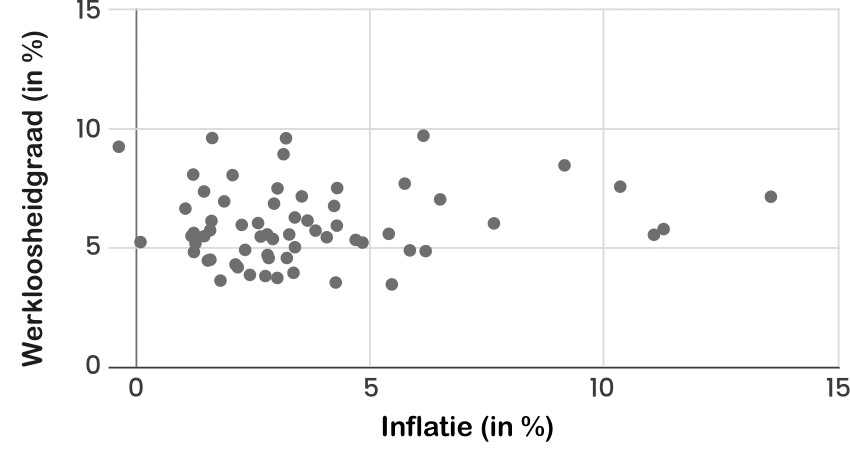
\includegraphics[width=\textwidth]{figures/fig1-1.png}
\caption[Relatie tussen werkloosheid en inflatie]{Relatie tussen werkloosheid en inflatie\index{inflatie}\footnotemark}
\label{fig1}
\end{figure}
\footautocite{11}


Ondanks decennia van opgestapeld bewijs dat het geen accurate verklaring is van hoe de wereld werkt, blijft deze theorie, tot op vandaag, echter bestaan. Rond 1970, toen wereldwijd zowel de inflatie\index{inflatie} als de werkloosheid toenamen, werd de Keynesiaanse trade-off zonder enige twijfel weerlegd. Maar het voordeel van economische wetenschap zonder systematische en herhaalbare methode van experimenteren en testen is dat theorieën na hun weerlegging altijd kunnen worden aangepast op een manier die afwijkende waarnemingen in de echte wereld goed praten. Dat is de essentie van pseudowetenschap.

Hilarisch genoeg pasten de Keynesianen hun theorie aan door er simpelweg een nieuwe term ``aanbodschok'' in op te nemen. Een aanbodschok is een onsamenhangende term, achteraf gemaakt als een rechtvaardiging om te verklaren hoe stijgingen in werkloosheid en inflatie\index{inflatie} tegelijkertijd kunnen voorkomen. Sindsdien zijn de wereldeconomieën getuige geweest van elke denkbare combinatie van inflatie\index{inflatie}- en werkloosheidscijfers, en de Keynesianen hebben met succes de waan in stand gehouden dat er zo’n trade-off tussen werkloosheid en inflatie\index{inflatie} bestaat. Elke afwijking van deze relatie kan worden verklaard door een aanbodschok of diverse andere denkbare substituten te hulp te roepen, en dus is er geen observatie mogelijk die deze relatie weerlegt. Het verklaart alles en verklaart daarom niets. De illusie van economie als een precieze, kwantitatieve en empirische wetenschap wordt alleen in stand gehouden door de theorieën vrij te stellen van empirisch onderzoek in de echte wereld.

\textbf{Na een eeuw natuurkunde te hebben nagebootst en klassieke methodologische grondslagen te hebben losgelaten, is de economie er niet in geslaagd om één kwantitatieve wet of formule te produceren die onafhankelijk getoetst en gerepliceerd kan worden.} Macro-economische formules komen en gaan met de modes van moderne ideologische stromingen, maar geen enkele is objectief gemeten en gerepliceerd op een manier waardoor het een wetenschappelijke wet genoemd kan worden. Dat macro-economie centrale regeringen macht geeft en academici verrijkt, kan helpen verklaren waarom het heeft standgehouden.

\section{Een contrast van benaderingen}

Om de benadering van het menselijk handelen\index{menselijk handelen} van de economische discipline te illustreren en te vergelijken met de moderne kwantitatieve economische methodologie, kunnen we als voorbeeld de kwestie van door de overheid\index{overheid} opgelegde minimumlonen nemen, die een ondergrens opleggen aan wat werkgevers hun werknemers kunnen betalen. Dit is een populaire beleidsinterventie in het grootste deel van de wereld, en de tegengestelde perspectieven hierop dienen als een les binnen de twee verschillende kaders voor het denken over economie: menselijk handelen\index{menselijk handelen} en aggregaten.

Stel je een politicus voor die verkiezingen wil winnen in een land zonder minimumloonwetten. Zoals in alle tijden en plaatsen in de menselijke geschiedenis is er een natuurlijke variatie in de lonen van arbeiders. De politica besluit haar campagne te richten op het verbeteren van de levensstandaard van de armsten uit de samenleving door een minimumloon te verplichten, waarvan ze zich voorstelt dat het de ontvangers ervan een fatsoenlijk bestaan garandeert. Op basis van haar macro-economische raamwerk dat gericht is op aggregaten, besluit de aspirant-leider een minimumloon van \$10 per uur op te leggen. De econoom concludeert dat 20\% van alle werknemers, die 35\% van de bevolking onderhouden, momenteel minder dan \$10 per uur verdienen. Het totale effect van het opleggen van het minimumloon zou leiden tot een loonstijging van \$10 miljard per jaar. Op basis van geavanceerde historische en theoretische modellen schat de econoom verder dat de stijging van de lonen met \$10 miljard zich zou vertalen in een stijging van de consumentenbestedingen met \$8 miljard, waarvan de modellen schatten dat dit zou resulteren in de creatie van 40.000 nieuwe banen, een stijging van de industriële productie\index{productie} met 12\%, een stijging van de export met 4\% en een stijging van het bruto binnenlands product met \$16 miljard.

Volgens deze collectivistische benadering van economische analyse zijn de aggregaten de causale factoren in economische fenomenen, en handelen ze volgens de theoretische relaties die door economen zijn vastgesteld, op een vergelijkbare manier als hoe natuurkundigen en scheikundigen wetenschappelijke regels vaststellen. Deze conclusies zijn tot stand gekomen met behulp van wetenschappelijk ogende vergelijkingen die niet veel verschillen van de vergelijkingen die gebruikt worden in de algemene gaswet. In het kader van de geaggregeerde economische analyse klinkt de wet op het minimumloon als een grote zegen voor de samenleving. De armste werknemers zullen hun levensstandaard aanzienlijk verhogen, sommige werklozen zullen werk vinden als gevolg van de extra uitgaven, en de hele samenleving wordt productiever. Bovendien stijgt de export, wat de economie aan buitenlandse valuta helpt.

Als dit te mooi klinkt om waar te zijn, dan is dat omdat het niet waar is. De dingen zien er anders uit door de lens van de econoom met de Mises-bril. De deugdelijke econoom weet dat menselijk handelen\index{menselijk handelen} de drijvende kracht achter menselijke zaken is en analyseert de wereld niet door middel van geaggregeerde grootheden. In plaats daarvan analyseert hij beslissingen van echte mensen die door deze nieuwe wet worden beïnvloed. Werkgelegenheid is een overeenkomst tussen twee individuen; de werkgever en de werknemer. Een deugdelijk econoom begrijpt dat de keuze van een ondernemer om iemand in dienst te nemen, gebaseerd is op een eenvoudige rekensom: hij zal hem in dienst nemen als zijn bijdrage aan de bedrijfsinkomsten groter is dan zijn loon. Als het wettelijk minimumloon hoger is dan de marginale opbrengst van de werknemer, dan kost het in dienst nemen van de werknemer het bedrijf\index{bedrijf} geld en is het een soort donatie van het bedrijf\index{bedrijf} aan de werknemer. Werkgevers weten dat het aannemen van zo’n werknemer een dure misstap is, en werkgevers die dat niet weten, zullen snel zien dat hun bedrijf\index{bedrijf} failliet\index{faillissement} gaat, omdat het geld blijft verspillen aan lonen die het zich niet kan veroorloven. Alleen werkgevers die deze economische realiteit begrijpen, zullen werkgevers blijven, en zij die dat niet doen, zullen hun bedrijf\index{bedrijf} verliezen. Emotionele chantage door politici kan niets aan deze realiteit veranderen.

Lonen zijn, net als alle prijzen op een markt, niet zomaar willekeurige getallen die door hebzuchtige werkgevers worden gekozen. Ze zijn een weerspiegeling van de marginale productiviteit van de werknemer. Nu de wet bepaalt dat een werknemer \$10 per uur moet krijgen, moet de werkgever opnieuw overwegen of het de moeite waard is om deze werknemer in dienst te nemen. Wanneer de overheid\index{overheid} een minimumloon oplegt, verandert dat niet op magische wijze de calculus van de werkgever, noch verhoogt het op magische wijze de productiviteit van de werknemer. De werkgever zal nog steeds alleen werknemers aannemen wiens productiviteit hoger is dan hun loon. De wet op het minimumloon maakt het dus illegaal voor werkgevers om iemand in dienst te nemen wiens marginale productiviteit minder is dan \$10 per uur. Elke werknemer met een lagere productiviteit zal nu een verlies betekenen voor elk bedrijf\index{bedrijf} dat hem in dienst neemt en hem dat bedrag betaalt. Of hij wordt ontslagen, of het bedrijf\index{bedrijf} dat hem inhuurt, verliest geld en gaat failliet\index{faillissement}. In alle gevallen worden deze banen geëlimineerd, en iedereen met een productiviteit van minder dan \$10 per uur is nu wettelijk werkloos; ofwel werkloos of illegaal tewerkgesteld.

Bekeken door de lens van menselijk handelen\index{menselijk handelen}, is het effect van een minimumloonwet dat het voor werknemers met een lage productiviteit illegaal wordt om een baan te krijgen, en veel van deze werknemers zullen hun baan verliezen. Als we verder kijken door de lens van menselijk handelen\index{menselijk handelen}, dan zien we dat de werknemers die hun baan verliezen de werknemers zijn met de laagste productiviteit in de samenleving, en dit zijn meestal de armste, jongste en minst ervaren werknemers. Door het voor hen illegaal te maken om te werken, wordt het voor hen in feite illegaal om hun productiviteit te verhogen door tijdens het werk te leren en waardevolle werkervaring op te doen. Minimumloonwetten zijn dus bijzonder schadelijk voor de mensen die het meest behoefte hebben aan werk, en ze zijn een factor die bijdraagt aan het ontstaan van grootschalige werkloosheid en ongeschiktheid voor de arbeidsmarkt. Een andere mogelijke implicatie is dat sommige bedrijven, vooral de bedrijven die voor hun bedrijfsvoering afhankelijk zijn van deze laagbetaalde arbeiders, hogere lonen zouden betalen, maar ook de prijzen van hun goederen zouden verhogen om de hogere lonen te financieren. Consumenten zouden dan de prijs\index{prijs} betalen door hogere productprijzen en een lagere hoeveelheid beschikbare goederen. In dit scenario wordt elke potentiële stijging van het inkomen van een werknemer met een laag loon tenietgedaan door een overeenkomstige stijging van de kosten van de goederen die hij moet consumeren.

Al deze gevolgen van minimumloonwetten zijn af te leiden door deugdelijke economen die de loonwet analyseren en de gevolgen ervan voor rationeel handelende individuen evalueren. Dit blijkt een veel nuttigere en nauwkeurigere beoordeling van de situatie te zijn dan alles wat we met wiskundige verhoudingen tevoorschijn kunnen toveren. Prijzen zijn een weerspiegeling van de onderliggende marktrealiteit die door menselijk handelen\index{menselijk handelen} wordt gestuurd. De onderliggende marktrealiteit veranderen door de weerspiegeling ervan te veranderen, werkt niet. Elke poging om prijscontroles door te voeren is mislukt omdat dit soort centrale planning de rol van menselijk handelen\index{menselijk handelen} negeert. Prijscontroles behandelen de economie alsof het over materiële objecten gaat, in plaats van menselijk handelen\index{menselijk handelen}. Schuettinger en Butler hebben een deprimerende, maar onderhoudende geschiedenis van prijscontroles geschreven in \textit{Forty Centuries of Price Controls}, waarin ze illustreren hoe deze exacte dynamiek zich in culturen en naties door de geschiedenis heen heeft herhaald.\autocite{12} Koningen, keizers, politici en bureaucraten zien de wereld van economische transacties als een onmenselijk proces dat ze naar gelang hun behoeften kunnen veranderen. Zij oordelen dat de waarneembare marktverschijnselen binnen aanvaardbare grenzen blijven. Ze gaan ervan uit dat mensen gewoon hun handelen zullen aanpassen om ervoor te zorgen dat deze wetten worden nageleefd. In werkelijkheid passen mensen hun handelingen aan om hun eigen welzijn te optimaliseren, niet om bureaucraten tevreden te stellen. De handelaar verkoopt liever helemaal niet dan met verlies. Je ziet ofwel de vrije marktprijs of je ziet helemaal geen marktprijs. In deze laatste economie komen echte prijzen tot stand op zwarte markten\index{markten}.

Deugende economen begrijpen dat waarneembare economische verschijnselen en statistieken slechts manifestaties zijn van het onderliggende handelen van de betrokken mensen. Mensen proberen voortdurend hun eigen levenssituatie te verbeteren en het is zinloos om hen te verplichten tegen hun eigen belangen in te handelen. Wetten opleggen die tegen het eigenbelang van mensen ingaan, verandert de menselijke natuur niet. Het vermindert de stimulans om zich legaal te gedragen en vernietigt zo het respect van de maatschappij voor wetten. Dit essentiële besef is de reden waarom de deugdelijke econoom voorstander is van individuele economische vrijheid en tegen de beperking ervan door overheden. De menselijke geest is ontembaar en zal niet handelen op een manier die schadelijk is voor zichzelf.

Een goede econoom begrijpt dat mensen voortdurend handelen om hun lot in het leven te verbeteren. Het opleggen van wettelijke straffen op elke vreedzame economische activiteit die ze zouden kunnen kiezen, kan niet leiden tot een verbetering van hun leven, omdat dit simpelweg de keuze aan handelingen die voor hen beschikbaar zijn, zal beperken en verkleinen.

Geaggregeerde analyse verblindt de nepeconoom voor de gevolgen van deze wetten voor de mensen wier vrijheden beperkt worden. Na het formuleren van wiskundige maatstaven voor sociale verschijnselen, neemt de collectivistische econoom vervolgens aan dat deze maatstaven oorzakelijke factoren zijn in het vaststellen van menselijke zaken.

De wereld heeft al veel te veel economische leerboeken die zijn geschreven in de pseudowetenschappelijke kwantitatieve traditie. Dit boek zal daar zeker niet bij horen. Het zal niet proberen om economie uit te leggen in de taal van de natuurwetenschappen, en het zal geen verfijnde aggregaatvergelijkingen bevatten. Dergelijke benaderingen beloven veel, maar leveren weinig betrouwbare, bruikbare inzichten op.

\chapter{Waarde}

\begin{blockquotebox}
    Waarde is dus niet inherent aan goederen. Het is geen eigenschap ervan, noch iets wat onafhankelijk op zichzelf bestaat. Het is een oordeel dat economisch\index{economisch} handelende mensen vellen over het belang van de goederen die ze tot hun beschikking hebben voor het behoud van hun leven en welzijn. Daarom bestaat waarde niet buiten het bewustzijn van mensen.\footnotemark
    \par\raggedleft--- Carl Menger\index{Carl Menger}
\end{blockquotebox}
\autocite{13}

\lettrine{H}et eerste hoofdstuk was een methodologische inleiding tot het onderwerp economie en illustreerde de Oostenrijkse benadering waarin menselijk handelen\index{menselijk handelen} centraal staat. In dit hoofdstuk gaan we in op de kern van het vakgebied economie, de basisbegrippen en de belangrijkste vraagstukken die het vakgebied probeert te beantwoorden.

Aan het einde van de negentiende eeuw legde de Oostenrijkse econoom Carl Menger\index{Carl Menger} de fundamenten voor de moderne economie. Zijn verklaringen over de subjectieve natuur van waarde en economische keuzes, samen met de introductie van marginale analyse, zorgden voor een revolutionaire verandering binnen het domein. Deze concepten boden een stevige theoretische en methodologische grondslag die een systematische analyse mogelijk maakte van de manier waarop mensen economische\index{economisch} beslissingen nemen.\footnote{Nvdr. Economiseren, of economisch\index{economisch} handelen, houdt in dat men bewuste keuzes maakt met het doel middelen optimaal te benutten en een balans te vinden tussen behoeften en de beschikbare middelen.} Dit ondanks het feit dat economie als studiegebied al sinds de tijd van Aristoteles bestond. Mengers baanbrekende werk zorgde voor een dieper inzicht in de impact van economische activiteiten op het menselijk leven. Zijn leerboek \textit{Principles of Economics}, gepubliceerd in 1871, is wellicht het oudste economische leerboek dat vandaag de dag nog steeds van belang en leesbaar is. Dit hoofdstuk biedt een overzicht van enkele kernconcepten uit Mengers werk, waarbij zijn definities worden gebruikt als fundament voor de analyse van thema's die in latere hoofdstukken worden behandeld. Daarna worden de essentiële Mengeriaanse concepten besproken die ten grondslag liggen aan economische analyse: subjectieve waarde\index{subjectieve waarde} en marginale analyse.

\section{Nut en waarde}
\subsection{Goederen}

Menger omschrijft een goed als iets bruikbaars dat ingezet kan worden om menselijke behoeften te bevredigen. Voorwaarden om iets als een goed te beschouwen zijn: ten eerste moet er sprake zijn van een menselijke behoefte; ten tweede moeten de kenmerken van het goed in staat zijn deze behoefte te vervullen; ten derde is het noodzakelijk dat men zich bewust is van deze causale relatie; en ten slotte moet men over het goed kunnen beschikken in voldoende mate om de betreffende behoefte te kunnen bevredigen.

\subsection{Nut}

Nut is het vermogen van een goed om menselijke behoeften te bevredigen. Nut hangt af van ons vermogen om het verband te begrijpen tussen een goed en de behoefte die het vervult. Nut is een algemene voorwaarde om een object een goed te laten zijn. Alleen als iets nut kan bieden, kan het door mensen als een goed worden beschouwd.

\subsection{Schaarste}
Goederen kunnen worden onderverdeeld in twee categorieën, economische en niet-economische. Het onderscheid tussen de twee is \textbf{schaarste\index{schaarste}}: de vraag naar economische goederen is altijd groter dan het geleverde aanbod, terwijl bij niet-economische goederen het aanbod groter is dan de door mensen gevraagde hoeveelheden. 

Een \textbf{niet-economisch\index{economisch} goed} is een goed dat beschikbaar is in hoeveelheden die groter zijn dan de vraag ernaar, waardoor rivaliteit of concurrentie om het goed te bemachtigen uitgesloten is. Het beste voorbeeld is zuurstof, dat essentieel is voor het overleven van de mens, maar desondanks overal waar mensen leven in overvloed aanwezig is.\footnote{Het is schaars bij het onder water duiken en in de ruimte, en daarom wordt het in deze omgevingen een economisch\index{economisch} goed, waarvoor een geavanceerde infrastructuur nodig is om het beschikbaar te maken.} Zuurstof is daarom geen economisch\index{economisch} goed.

Omdat een \textbf{economisch\index{economisch} goed} schaars is, zal de vraag ernaar groter zijn dan het aanbod, en dit creëert rivaliteit om het te verkrijgen, waardoor mensen gedwongen worden om keuzes te maken tussen dit goed en andere goederen. De schaarste\index{schaarste} van economische goederen dwingt mensen om te \textbf{economiseren} en keuzes te maken tussen schaarse alternatieven. Economiseren, of het economisch\index{economisch} handelen, verwijst volgens Menger naar de neiging van mensen om zo groot mogelijke hoeveelheden te hebben van de goederen die hun behoeften kunnen bevredigen, om de nuttige functies van deze goederen te behouden, om hun meest dringende behoeften voorrang te geven boven minder dringende, en om de grootste voldoening te verkrijgen uit de hoeveelheid van een goed.

\subsection{Economie}

Economie is de \textbf{studie van menselijke keuzes bij schaarste\index{schaarste}}. Het richt zich op het analyseren van hoe mensen oplossingen proberen te vinden voor het probleem van het verschil tussen wat ze hebben en wat ze willen, en de gevolgen van hun keuzes. 

Omdat schaarste\index{schaarste} een permanent bestaansgegeven is, maken mensen voortdurend keuzes tussen verschillende manieren van handelen, verschillende goederen en verschillende behoeften om te bevredigen. De noodzaak om deze keuzes te maken dwingt ons om het nut dat we ontlenen aan verschillende goederen tegen elkaar af te zetten, zodat we weloverwogen keuzes kunnen maken.

\subsection{Waarde}

Waarde is onze subjectieve beoordeling van de voldoening die we uit goederen halen, of verwachten te halen. Het stelt ons in staat om economische beslissingen te nemen. Menger definieert waarde als “het belang dat individuele goederen of hoeveelheden goederen voor ons hebben, omdat we ons ervan bewust zijn dat we afhankelijk zijn van de beschikking erover voor de bevrediging van onze behoeften.”\autocite{15} Waarde is volgens Menger ook “het belang dat we eerst toekennen aan het vervullen van onze behoeften, namelijk aan ons leven en ons welzijn en als gevolg daarvan overdragen op economische goederen als de exclusieve oorzaken van de bevrediging van onze behoeften.”\autocite{16}

\subsection{Subjectieve waarde}

De basis van economische analyse, en een van de baanbrekende inzichten uit het werk van Menger, is dat \textbf{waarde subjectief is}. Het bestaat alleen in de geest van de persoon die de waarde bepaalt. Zoals Menger het stelde: “Waarde is dus niet inherent aan goederen, geen eigenschap ervan, noch een onafhankelijk iets wat op zichzelf bestaat. Het is een oordeel dat economiserende mensen vellen over het belang van de goederen die ze tot hun beschikking hebben voor het behoud van hun leven en welzijn.”\autocite{17}

Het is niet een inherente aard van goederen die ze waardevol voor ons maakt, maar alleen onze beoordeling van hun geschiktheid om aan onze behoeften te voldoen. Naarmate hun vermogen om aan onze behoeften te voldoen verandert, verandert ook hun waarde voor ons. Waarde is dus geen fysieke of chemische eigenschap van economische goederen; het is een psychische eigenschap die ze alleen krijgen wanneer mensen ze beoordelen. In de beroemde woorden van Menger: “Waarde bestaat niet buiten het bewustzijn van de mens.”\autocite{18}

Mijn favoriete voorbeeld om de subjectieve aard van waarde te illustreren is olie\index{olie}. Tot in de negentiende eeuw verminderde de aanwezigheid van olie\index{olie} de waarde van een stuk land, omdat de olie\index{olie} eerst weggehaald moest worden voordat het land gebruikt kon worden voor landbouw, handel of woningbouw. Zolang de mens olie\index{olie} als een vervuiling zag, had olie\index{olie} een negatieve economische waarde. Toen mensen zich realiseerden dat geraffineerde olie\index{olie} in een verbrandingsmotor gebruikt kon worden om machines aan te drijven die aan hun behoeften aan transport, elektriciteit en warmteopwekking voldeden, veranderde olie\index{olie} van hinderlijke overlast in een enorm waardevol en essentieel product, waar niemand in de moderne wereld nu zonder kan. Olie in het jaar 2020 verschilt chemisch en fysiek niet van olie\index{olie} in het jaar 1620, en toch is de waarde ervan veranderd van negatief naar positief. Hoewel onze bewuste inschatting van onze behoeften de fysische en chemische eigenschappen van olie\index{olie} niet kan veranderen, kan het de economische waarde ervan wel veranderen. Olie veranderde van een negatieve in een positieve waarde toen het menselijke bewustzijn het als nuttig herkende. Zoals Menger het stelt: “De waarde van goederen vloeit voort uit hun relatie tot onze behoeften, en is niet inherent aan de goederen zelf. Met veranderingen in deze relatie ontstaat en verdwijnt waarde.”\autocite{19}

Om dit punt verder te illustreren: terwijl dit boek in 2020 geschreven wordt, is een aanzienlijk deel van de wereldbevolking onderworpen aan regeringen die in de hele wereld aanzienlijke en verstikkende beperkingen van vrij maatschappelijk verkeer en economische productie\index{productie} opleggen. Olie wordt geproduceerd voor onmiddellijke consumptie\index{consumptie} en er is zeer weinig reservecapaciteit voor de opslag ervan in verhouding tot de enorme verbruikte hoeveelheden. Toen de industrie en het transport vrijwel tot stilstand kwamen, kon de overtollige olieproductie nergens heen, de olieprijs kelderde en werd zelfs een paar dagen negatief. Gezien het grote aanbodoverschot vergeleken met de vraag en het gebrek aan opslagcapaciteit, werd het bezitten van olie\index{olie} weer een last, zoals in het pre-industriële tijdperk, en de eigenaars moesten opnieuw betalen om het kwijt te kunnen. De olieprijs werd al snel weer positief en bleef stijgen. Er veranderde niets aan de inherente eigenschappen van olie\index{olie} toen de prijs\index{prijs} van negatief naar positief naar negatief naar weer positief ging; de omstandigheden van de mensen die de waarde vaststellen veranderden, en zo ook hun subjectieve waarderingen.

Zoals het voorbeeld van olie\index{olie} illustreert, kan waarde niet bestaan buiten de menselijke waardering en keuzes die hun voorkeuren weerspiegelen. Waarde kan geen constante eigenschap van objecten zijn; het is een bewust fenomeen in onze geest. Dit betekent niet dat waarde niet echt is. Waarde is echt en betekenisvol, en zij bepaalt onze handelingen en beslissingen die richting geven aan de productie\index{productie}, consumptie\index{consumptie} en het gebruik van de echte materiële objecten in onze wereld. Mengers erkenning van de subjectieve aard van waarde was een zeer belangrijk keerpunt in het economisch\index{economisch} denken. Economen uit het verleden hadden moeite om uit te leggen hoe goederen gewaardeerd werden en waarom bepaalde goederen waardevoller waren dan andere. Al deze mysteries en paradoxen rondom waardering werden pas opgelost met het Mengeriaanse inzicht van subjectieve waardering en marginale analyse.

\section{Waardering: ordinaal en kardinaal}

De eerste belangrijke implicatie van de subjectieve aard van waarde is dat deze niet objectief gemeten en uitgedrukt kan worden. Aangezien de menselijke beoordeling van waarde subjectief is en voortdurend verandert op basis van onze behoeften en ons begrip van de mogelijkheden van goederen om aan onze behoeften te voldoen, variëren waarderingen van persoon tot persoon; ook veranderen individuele waarderingen voortdurend afhankelijk van individuele omstandigheden. Om enige meting objectief vast te stellen, is een wetenschappelijke eenheid nodig als standaardmaat waartegen verschillende objecten worden beoordeeld, zoals besproken in Bijlage 1.

Gewicht, lengte, temperatuur en andere wetenschappelijke maten worden bepaald in objectief definieerbare eenheden die een nauwkeurige vergelijking tussen verschillende objecten mogelijk maken. Maar een dergelijke eenheid kan niet bestaan voor menselijke waardering, omdat de waarde van een goed geen inherente objectieve eigenschap van het goed is. Het is een subjectieve psychische eigenschap die afhankelijk is van de persoon die de waardering uitvoert, afhankelijk van de steeds veranderende omstandigheden die het nut van dat goed bepalen met betrekking tot het bevredigen van behoeften. Er is geen objectieve standaard waarmee de voldoening van mensen vergeleken kan worden, omdat de individuen zelf de beoordelaars van de waarde zijn. Met andere woorden, er is geen manier om de voldoening die een persoon uit een goed haalt objectief te meten in termen van de voldoening die een andere persoon uit hetzelfde goed haalt.

Zonder een standaard objectieve eenheid is meten onmogelijk, en waardering kan niet worden uitgedrukt in objectieve numerieke \textbf{kardinale} termen, waardoor het onmogelijk is om economische waarde met wiskundige precisie te meten. Zonder een constante eenheid als referentie voor waarde die voor iedereen vast te stellen is, is het niet mogelijk om de economische waarde van verschillende goederen ten opzichte van elkaar uit te drukken. Het is mogelijk om de lengte van verschillende voorwerpen te meten, omdat ze allemaal gemeten kunnen worden aan de hand van de constante referentie van een inch, voet, mijl of meter. Iemand die een koelkast in een keuken wil installeren, kan de toegewezen ruimte van de koelkast meten in centimeters en vervolgens de afmetingen van de koelkast opzoeken om te zien of deze zou passen. Zo’n meting is zinvol en nuttig omdat de klant en de fabrikant van de koelkast een zeer nauwkeurige en precieze gedeelde definitie hebben van wat een centimeter is. Zonder overeenstemming over een gemeenschappelijke constante eenheid zou het onmogelijk zijn om, zonder de koelkast te plaatsen, te weten of hij zou passen.

Zonder een gemeenschappelijke constante eenheid is de enige manier waarop we waarde kunnen uitdrukken \textbf{ordinaal}, waarbij goederen met elkaar worden vergeleken en gerangschikt op basis van de voorkeur van het waarderende individu, maar niet expliciet kwantitatief worden gewaardeerd. Het is mogelijk voor een individu om zijn voorkeur voor het ene goed boven het andere te kennen, omdat er een constante is voor deze vergelijking – het individu dat de waardering doet. Het is dus mogelijk om goederen te \textit{vergelijken} in termen van waarde, aangezien een individu gemakkelijk kan bepalen of hij meer waarde hecht aan goed A dan aan goed B, en meer aan goed B dan aan goed C. Maar deze waardering is puur subjectief, uitgedrukt in verhouding tot het nut dat de persoon die het waardeert, ervaart. Het is onmogelijk voor de persoon om deze voorkeuren in kwantitatieve en kardinale termen uit te drukken, zoals het waarderen van goed A met een precieze numerieke waarde uitgedrukt in dezelfde eenheid waarmee de voorkeur voor goed B wordt uitgedrukt. In de echte economie kan er niet zoiets bestaan als een verklaring die de waarde van goederen weergeeft, zoals \enquote{de waarde van A = 14,372x, de waarde van B = 4,258x, en de waarde van C = 1,273x,} waarbij x een objectieve waarde-eenheid is die gebruikt kan worden voor persoonlijke en interpersoonlijke nutsvergelijkingen.

Zoals Mises het stelt:

\begin{blockquotebox}
    Er is een meer en een minder in het wegnemen van gevoelens van ongemak; maar hoeveel de ene voldoening de andere overtreft, kan alleen maar gevoeld worden; het kan niet op een objectieve manier vastgesteld en bepaald worden. Een waardeoordeel meet niet, het ordent in een schaal van graden, het rangschikt. Het drukt een voorkeursvolgorde uit, maar geen maat en gewicht. Alleen de rangtelwoorden kunnen erop worden toegepast, maar niet de kardinale getallen.\footnotemark
\end{blockquotebox}
\autocite{20}

Denk aan de manier waarop je persoonlijk dingen ten opzichte van elkaar waardeert. Ben je in staat om ze uit te drukken in één eenheid die ze allemaal meet? Kunnen alle dingen die je waardeert, van materiële goederen tot vriendschappen, familie en geluk, gemeten worden in dezelfde eenheid? Bestaat er een vaste wisselkoers\index{wisselkoers} tussen een familielid en materiële goederen? Kun je jouw kind waarderen op basis van een geldhoeveelheid? Hoeveel auto’s heeft een mens nodig om voor zijn kind te ruilen? Menselijke waarden kunnen niet gemeten worden met één gestandaardiseerde eenheid. Menselijke waarderingen kunnen alleen vergeleken worden, maar ze kunnen niet opgeteld, afgetrokken of vermenigvuldigd worden. Zonder een gemeenschappelijke en constante eenheid zijn metingen en wiskundige bewerkingen niet mogelijk.


\section{Waarde en prijs\index{prijs}}

De waarde van economische goederen staat los van hun prijs\index{prijs} en mag hier ook niet mee verward worden. De prijs\index{prijs} van een economisch\index{economisch} goed is niet de objectieve waardering ervan, noch de subjectieve waardering van een van de partijen die handel drijven. De prijs\index{prijs} waartegen een verkoop plaatsvindt, illustreert alleen dat de verkoper het goed minder waardeert dan de prijs\index{prijs}, terwijl de koper het meer waardeert. Als dit niet het geval was geweest, zou de transactie niet hebben plaatsgevonden.

Een veelgemaakte fout in de economie is om waarde en prijs\index{prijs} door elkaar te halen. Die fout gaat gepaard met het idee dat waarde inderdaad objectief gemeten kan worden, uitgedrukt in monetaire eenheden. Maar dat kan niet kloppen, omdat marktprijzen alleen een grens aangeven voor de waarde van goederen, die strikt zijn gebonden aan een bepaalde tijd en plaats. Wanneer iemand ermee instemt om een goed voor \$1.000 te verkopen, geeft ze daarmee aan dat ze het goed op minder dan \$1.000 waardeert. Als ze het voor meer dan \$1.000 had gewaardeerd, zou ze niet geïnteresseerd zijn geweest om het voor \$1.000 te ruilen. Alleen als haar waardering lager is dan \$1.000, zou een bod van \$1.000 haar overhalen om te verkopen. Omgekeerd, als de koper \$1.000 uitgeeft om dat goed te kopen, is het enige dat we over zijn waardering van het goed kunnen zeggen dat die hoger is dan \$1.000, anders zou hij dat bedrag er niet voor betaald hebben. Het is niet mogelijk om de precieze waardering van een individu te bepalen op basis van zijn transactie, maar alleen de boven- of ondergrens ervan. Alleen al de ruil\index{ruil} vertelt ons veel over waardering.

\section{Vrije ruil\index{ruil}}

Wanneer twee mensen er vrij voor kiezen om economische goederen te ruilen, moet het noodzakelijkerwijs waar zijn dat ze allebei geloven dat ze voordeel zullen halen uit de ruil\index{ruil}; anders zouden ze niet ruilen. Wederzijds voordelige ruil\index{ruil} geeft aan dat elke partij iets heeft ontvangen waar ze meer waarde aan hechten dan wat ze hebben opgegeven. De enige manier waarop dit mogelijk is, is als we begrijpen dat ze allebei verschillende subjectieve waarderingen van het geruilde goed hebben. Als de waarde van deze goederen objectief zou zijn, zou deze niet van persoon tot persoon verschillen, en zou de ruil\index{ruil} niet mogelijk zijn, omdat geen van beiden vrijwillig zou kiezen om het goed met de objectieve lagere waarde te accepteren in ruil\index{ruil} voor het goed met de hogere objectieve waarde. Dit wordt meer in detail besproken in Hoofdstuk 9 over handel, waarin de voordelen van ruilhandel\index{ruilhandel} worden geïllustreerd.

\section{Bepalende factoren van waarde}

Het fundamentele verschil tussen economen van de Oostenrijkse School\index{Oostenrijkse School} en andere scholen is dat Oostenrijkers waarde als subjectief beschouwen, terwijl andere scholen waarde als iets objectiefs zien, of objectief meetbaar. Om die schijn in stand te houden, definiëren sommige moderne economieboeken waarde als een functie van nut, wat gemeten wordt in een denkbeeldige en ongedefinieerde eenheid genaamd \textit{util}.\footnote{Nvdr: Nutseenheid} Er is geen standaard voor wat een util is, en geen manier om iets te meten in termen van utils. Sommige moderne wiskundige economen drukken waarde uit in expliciete numerieke termen, gemeten in monetaire eenheden, waarbij ze waarde verwarren met prijs\index{prijs} en niet kunnen verklaren waarom mensen transacties zouden aangaan om voorwerpen te ruilen als beide voorwerpen identieke waarden hebben. Marxisten daarentegen denken dat waarde bepaald wordt door de arbeid die in de productie\index{productie} van een goed gaat zitten. Dit is een absurde stelling volgens welke dingen waardevol worden als er werk in gestoken wordt om ze te produceren, ongeacht of iemand ze wil bezitten. Als je evenveel tijd zou besteden aan het bakken van een normale cake als aan het bakken van een cake van modder, dan zou de marxist beweren dat beide cakes dezelfde waarde zouden hebben.

Er gaat een intuïtieve aantrekkingskracht uit van het idee dat arbeid waarde bepaalt. We kunnen zien dat economische goederen altijd een bepaald element van arbeid vereisen om ze aan de menselijke behoeften te laten voldoen. Zelfs fruit dat in het wild groeit, vereist dat de mens de nodige arbeid verricht om het te plukken en op te eten voordat het aan zijn behoeften kan voldoen. Het is niet mogelijk om goederen te bedenken die menselijke behoeften bevredigen zonder dat er arbeid aan wordt besteed, en dit brengt de aanhangers van de arbeidstheorie tot de conclusie dat het arbeid is die waarde geeft aan goederen en dat waarde gemeten kan worden aan de hoeveelheid arbeid die eraan wordt besteed. Echter, dit is een onhoudbaar idee. 

Men waardeert goederen alleen op basis van hun capaciteit om in onze behoeften te voorzien. Bij een aankoop interesseert de tijd en moeite die in het vervaardigen van een product is gestoken de koper niet; hij kijkt enkel naar de diensten en het nut dat het product voor hem heeft. Producenten zetten arbeid in met de verwachting dat dit de consument waarde zal brengen, maar arbeid leidt niet automatisch tot waardevermeerdering. Arbeid kan men verspillen aan een productieproces\index{productieproces} dat faalt en geen bruikbaar product voortbrengt. De inspanning maakt de output niet waardevol; de nutteloosheid ervan maakt het onwaardeerbaar voor wie de waarde ervan probeert te bepalen. De hoeveelheid arbeid die men in productie stopt, garandeert niet de waarde ervan. Hoewel arbeiders hun arbeid kunnen over- of onderschatten, is het uiteindelijk de keuze van de consument op de markt die de waarde van goederen bepaalt. Producenten en arbeiders investeren hun arbeid in productieprocessen in de hoop waardevolle goederen te creëren. Als de kosten van de inputs lager zijn dan de marktprijs van de output, maakt de producent winst\index{winst}, wat aantoont dat haar investering maatschappelijk productief was omdat de input minder kostte dan de waarde van de output. Echter, als de marktprijs van het product lager is dan de kosten van de inputs, krijgt de producent een signaal dat haar productieproces destructief is, en hoe langer dit doorgaat, des te meer kapitaal\index{kapitaal} ze verspilt.

In de Oostenrijkse School\index{Oostenrijkse School} is waarde subjectief en afhankelijk van het tijdstip en de plaats waarop de waardering plaatsvindt. Waarde wordt afgeleid van menselijke keuzes die noodzakelijk zijn vanwege schaarste\index{schaarste}. Waarde wordt door individuen aan elke eenheid toegekend op het moment en de plaats waarop ze beslissingen nemen, maar het is geen universele eigenschap van het goed. Zonder een subjectieve opvatting van waarde is het niet mogelijk om coherente verklaringen te vinden voor waarom en hoe mensen de economische keuzes maken die ze maken. Hoe consumenten de subjectieve waarde\index{subjectieve waarde} van objecten bepalen, is aan hen. Hetzelfde individu zal hetzelfde goed op verschillende tijden en plaatsen verschillend waarderen, afhankelijk van vele factoren; met name hun bestaande voorraad van dat goed.

\section{Marginalisme}

Mengers andere significante bijdrage aan de economie is het concept van het marginalisme, ook wel bekend als de grensnutschool. Nadat Menger had vastgesteld dat de waarde van goederen niet inherent is aan de goederen zelf, maar eerder subjectief en afhankelijk van hun vermogen om aan onze behoeften te voldoen, paste hij dit toe op de studie van de waarde van verschillende eenheden van hetzelfde goed en legde daarmee de basis voor de moderne economische analyse. 

Aangezien de waarde van goederen wordt afgeleid van hun vermogen om aan onze behoeften te voldoen, en aangezien verschillende voldoeningen een ongelijke waarde voor ons hebben, zal de waarde van verschillende eenheden van hetzelfde goed ook ongelijk zijn, omdat deze afhangt van de behoeften waaraan ze voldoen. Hetzelfde goed zal voor dezelfde persoon een verschillende waarde hebben, afhankelijk van de behoefte waarin het op een bepaald moment voorziet.

Individuen gebruiken de eerste eenheid van een goed om te voldoen aan de belangrijkste en dringendste behoeften die ermee verbonden zijn. Ze zullen de tweede eenheid gebruiken om aan de op één na dringendste behoefte te voldoen. Naarmate de hoeveelheid van het goed dat ze bezitten toeneemt, worden de behoeften waaraan wordt voldaan minder waardevol en minder dringend. Met andere woorden, identieke goederen hebben verschillende waarden voor individuen, omdat het nut dat ze opleveren niet identiek is. De eerste eenheden zijn het waardevolst, en naarmate het aantal geconsumeerde eenheden toeneemt, is elke marginale eenheid minder waardevol dan de vorige.

Menger illustreerde dus dat de waarde die we aan goederen hechten niet afhankelijk is van hun totale of algemene nut en dat hun nut niet iets is dat inherent is aan deze goederen in abstracte zin, ongeacht hun hoeveelheden. Het belang dat we aan goederen hechten is onlosmakelijk verbonden met de hoeveelheid van die goederen, en hun hoeveelheid in verhouding tot het bestaande aanbod van het goed dat we tot onze beschikking hebben. Mensen nemen beslissingen niet op basis van het totale of abstracte nut van een object, maar op basis van het nut dat specifieke hoeveelheden van het goed bieden en hun vermogen om onze verschillende behoeften te bevredigen.

\section{Marginaal nut}

Hoewel Menger de term zelf nooit gebruikte, zou zijn leerling Friedrich von Wieser later de term “marginaal nut\index{marginaal nut}” introduceren om te verwijzen naar het belang dat gehecht wordt aan de minst belangrijke behoefte die door één eenheid van de beschikbare hoeveelheid van een goed wordt verzekerd. Mises definieert het door te zeggen: “We noemen dit gebruik van een eenheid van een homogeen aanbod waarvan de eigenaar `n' eenheden heeft, maar dat aanbod niet zou gebruiken als zijn voorraad één eenheid minder was, `n-1' eenheden, het minst dringende gebruik of het marginale gebruik. Het nut dat ervan wordt afgeleid wordt het marginale nut genoemd.”\autocite{21}

De eerste eenheid voedsel die iemand eet, is bijvoorbeeld extreem waardevol, omdat het het verschil is tussen verhongeren en overleven. De tweede eenheid voedsel zal het verschil zijn tussen louter overleven en goed gevoed zijn. Hoewel het nog steeds zeer waardevol is voor het individu, is de tweede eenheid niet zo waardevol als de eerste. Er zullen nog meer eenheden voedsel worden aangeschaft om van de smaak te genieten of voor sociale bijeenkomsten, die weliswaar waardevol zijn, maar niet zo waardevol als de vorige eenheden die werden gebruikt om te overleven en gezond te blijven. Als de voedselconsumptie van een individu blijft toenemen, komt hij uiteindelijk op een punt waarbij hij geen waarde meer hecht aan een extra eenheid voedsel en het liever niet heeft, zelfs als hij het gratis krijgt aangeboden. Een toename van het aantal geconsumeerde eenheden leidt ertoe dat de eenheden worden ingezet om aan minder dringende behoeften te voldoen, wat betekent dat elke opeenvolgende eenheid een lager nut heeft dan de vorige eenheid en dus een lagere waardering voor individuen. 

Met dit belangrijke inzicht weerlegde Menger het idee dat de waarde van goederen inherent is aan de goederen zelf. Hij illustreerde dat de waarde afhankelijk is van de behoeften waarin de goederen voorzien, die op hun beurt afhankelijk zijn van de overvloed en schaarste\index{schaarste} van de goederen, en alleen voor de persoon die de waarde bepaalt. Niemand wordt ooit gevraagd om het totale aanbod van een goed te waarderen, of om een goed abstract te waarderen. Economische beslissingen hebben alleen betrekking op individuele eenheden van goederen, en individuen nemen op elk moment in de tijd met name beslissingen over de volgende eenheid van een goed dat ze willen consumeren, niet over hun levenslange voorraad ervan, noch over het de abstracte versie van het goed zelf.

\section{Wet van afnemend marginaal nut\index{marginaal nut}}

Een belangrijke implicatie van Mengers benadering van waardering is de wet van afnemend marginaal nut\index{marginaal nut}. Deze wet stelt dat de waardering van een individu en het nut van een goed afnemen naarmate de hoeveelheid van het goed toeneemt. Aangezien individuen de eerste eenheden van een goed dat ze verwerven, gebruiken om de meest dringende behoeften te vervullen waarin het kan voorzien, moet hieruit volgen dat de eerste eenheid van een goed het hoogst gewaardeerd zal worden door dat individu. Naarmate hun bezit van dat goed toeneemt en elke marginale eenheid de minder dringende behoefte vervult, zal elke marginale eenheid een lagere waarde hebben voor het individu. De waarde die iemand aan een goed toekent, hangt op elk moment af van de behoefte die het vervult. Daarom zal de waardering voor iets verminderen naarmate men er meer van verkrijgt.

Dat het marginale nut van een goed afneemt naarmate de hoeveelheid toeneemt, is een belangrijk inzicht in de individuele besluitvorming. Iedereen die wel eens een dure aankoop heeft gedaan, kan zich dit voorstellen. Op de eerste dag dat je een nieuwe auto of nieuw speelgoed hebt, is de nieuwheidsfactor overweldigend en ben je erdoor gefascineerd. Dit wordt na verloop van tijd minder naarmate je meer gewend raakt aan de vele functies en eigenschappen. Wat nieuw was, wordt gewoon en verliest de allure die het had voordat je het ervoer. Je beleeft nog steeds plezier aan het besturen van de auto of het spelen met het speelgoed, maar het specifieke plezier neemt af met elk extra gebruik.

De wet van het afnemende marginale nut herinnert ons er nog eens aan dat er niet zoiets bestaat als een objectieve waarde van goed X, omdat die waarde verandert afhankelijk van de overvloed van goed X en de behoeften die ermee bevredigd worden. Er is altijd alleen een subjectieve waarde\index{subjectieve waarde} van de volgende (marginale) eenheid van goed X voor de persoon die de waarde bepaalt. Dit is afhankelijk van de subjectieve voorkeuren van het individu dat het waardeert en de schaarste\index{schaarste} van het goed.

\section{Waardering door het minst waardevolle gebruik}

Een andere implicatie van Mengers benadering van waardering: als individuen hun inventaris van een goed inzetten om aan hun meest dringende behoeften te voldoen, dan zal hun waardering van de marginale eenheid, hun waardering van de minst belangrijke bevrediging die dit goed verzekert, weerspiegelen. Bij het nemen van aankoopbeslissingen zal de waardering van een goed dus een weerspiegeling zijn van de waardering van de minst belangrijke bevrediging die het goed biedt. Iemand die besluit te betalen voor een maaltijd, zal dit niet betalen op basis van hoeveel waarde hij hecht aan voedsel op zichzelf of hoeveel waarde hij hecht aan al het voedsel dat hij in zijn leven heeft gegeten. Hij zal betalen naar de waarde die hij hecht aan de eerstvolgende maaltijd. De werkelijke waarde van al het voedsel zijn voor de man irrelevant. Als iemand heel zijn leven voldoende voedsel heeft gehad om gezond te blijven en op dit moment een nieuwe maaltijd kan eisen, dan waardeert hij de volgende eenheid voedsel niet net als al het voedsel dat hij tot nu toe heeft gegeten. Hij waardeert het niet alsof het het verschil is tussen leven en dood, want dat is het niet. De beslissing over de volgende maaltijd wordt gewaardeerd op basis van de behoefte die de volgende maaltijd voor deze persoon bevredigt, die, omdat het maar één maaltijd is, aanzienlijk lager zal zijn dan de waarde van voedsel dat hem in het algemeen in leven houdt of de waarde van alle voorgaande maaltijden die hem tot op heden in leven hielden. We kunnen dan zien hoe, wanneer we een keuze moeten maken over een bepaald goed, we het waarderen in het licht van het minst waardevolle gebruik dat mogelijk is, omdat dat de enige marginale keuze is die bestaat. Aan alle waardevollere toepassingen werd al voldaan met eerdere eenheden van eerder genuttigd voedsel. 

De persoon die overweegt om bijvoorbeeld een fles water van een restaurant te kopen, zal niet betalen op basis van de waarde die hij of zij aan water geeft om te overleven of om in zijn of haar dagelijkse basisbehoeften te voorzien. Ze beslissen gewoon over de marginale (volgende) eenheid water die ze gebruiken, nadat ze al andere eenheden water hebben toegewezen aan hun meer dringende behoeften. De prijs\index{prijs} die voor water wordt betaald, komt niet in de buurt van de waarde die het individu aan overleven hecht, omdat de beslissing om een fles water te kopen in een moderne stad alleen betrekking heeft op de consumptie\index{consumptie} van een extra fles water, en niet op overleven. Omdat water essentieel is voor het overleven van de mens, ontstaan alle menselijke samenlevingen alleen op plaatsen waar genoeg water is om aan de essentiële behoeften van de mensen te voldoen. Als deze behoeften verzekerd zijn, zal de prijs\index{prijs} van marginale eenheden niet de waarde van de basisbehoeften weerspiegelen, maar eerder de waarde van de minder dringende behoeften. Dit helpt ons te begrijpen waarom water relatief goedkoop is, ook al is het essentieel. De essentiële aard ervan zorgt ervoor dat mensen er meestal grote hoeveelheden van hebben en hun marginale aankoopbeslissingen baseren op de marginale eenheden die naar minder dringende behoeften gaan.

We kunnen zien waarom goederen die essentieel en belangrijk zijn om te overleven, meestal goedkoop zijn. In de moderne wereld betalen mensen niet voor water op basis van de waarde die ze hechten aan het overleven dankzij dat water. Ze leven al in een tijd en plaats die hun belangrijkste behoeften aan water tegen zeer lage prijzen veilig stelt. Hun individuele aankoopbeslissingen hebben betrekking op het verkrijgen van marginale hoeveelheden water die misschien een lichte dorst kunnen lessen, maar die niet nodig zijn om te overleven of gezond te blijven. Maar als je een individu in een situatie zou plaatsen waarin ze een paar dagen lang niet in staat is om water te kopen voor haar levensbehoeften, dan zou het minst waardevolle gebruik dat het haar zou bieden nog steeds het verschil zijn tussen leven en dood, en dat zou ervoor zorgen dat ze er veel waarde aan hecht. Zoals Mises uitlegt:

\begin{blockquotebox}
    De handelende mens bevindt zich niet in een positie waarin hij moet kiezen tussen al het goud\index{goud} en al het ijzer. Hij kiest op een bepaalde tijd en plaats onder bepaalde omstandigheden tussen een strikt beperkte hoeveelheid goud\index{goud} en een strikt beperkte hoeveelheid ijzer. Zijn beslissing om te kiezen tussen 100 ounce goud\index{goud} en 100 ton ijzer hangt helemaal niet af van de beslissing die hij zou nemen als hij zich in de hoogst onwaarschijnlijke situatie zou bevinden dat hij moet kiezen tussen al het goud\index{goud} en al het ijzer.
    \par\vspace{1em}\noindent
    Wat alleen telt voor zijn feitelijke keuze is of hij onder de bestaande omstandigheden de directe of indirecte voldoening die 100 ounce goud\index{goud} hem zou kunnen geven groter of kleiner acht dan de directe of indirecte voldoening die hij zou kunnen ontlenen aan 100 ton ijzer. Hij spreekt geen academisch of filosofisch oordeel uit over de absolute waarde van goud\index{goud} en ijzer; hij bepaalt niet of goud\index{goud} of ijzer belangrijker is voor de mensheid; hij perverteert niet als schrijver van boeken over de filosofie van de geschiedenis of over ethische principes. Hij kiest gewoon tussen twee voldoeningen die hij niet allebei tegelijk kan hebben.
    \par\vspace{1em}\noindent
    Wanneer de mens geconfronteerd wordt met het probleem van de waarde die moet worden toegekend aan één eenheid van een homogeen aanbod, beslist hij op basis van de waarde van het minst belangrijke gebruik dat hij maakt van de eenheden van het hele aanbod; hij beslist op basis van marginaal nut\index{marginaal nut}.\footnotemark
\end{blockquotebox}
\autocite{23}

\section{Water-diamantparadox}

Een belangrijke uitkomst van Mengers marginale analyse is dat het de eerste economische verklaring bood voor de water-diamantparadox\footnote{Ook bekend als de klassieke waardeparadox.}, een vraagstuk dat economen eeuwenlang had gepuzzeld. Hoe was het mogelijk dat water, onmisbaar voor het menselijk bestaan, vaak zeer goedkoop of zelfs gratis is, terwijl diamanten, die louter luxegoederen zijn en geen essentiële behoefte vervullen, zeer kostbaar zijn? Als waarde werkelijk subjectief is, waarom hechten mensen dan zoveel waarde aan zaken zoals diamanten die ze niet nodig hebben, terwijl ze relatief weinig waarde toekennen aan essentiële zaken zoals water? Zou een arbeidswaardetheorie, die stelt dat diamanten waardevoller zijn omdat hun productie\index{productie} meer arbeid vereist, niet logischer zijn?

Zoals eerder besproken, is de marktwaarde niet gebaseerd op een inherente eigenschap van het goed of de waarde van het totale aanbod; het is gebaseerd op de minst belangrijke behoefte die het goed vervult. Omdat drinkwater doorgaans in overvloed beschikbaar is op plekken waar mensen leven, zijn de meest urgente behoeften aan water al vervuld en worden op de markt beslissingen genomen over eenheden die veel minder dringende behoeften vervullen. Wanneer iemand in een moderne stad besluit geen fles water te kopen, ziet hij af van een kleine, op dat moment minder belangrijke behoefte aan water. Hij heeft nog steeds toegang tot het water dat nodig is voor zijn meest urgente en belangrijkste behoeften, zoals overleven en hygiëne. Diamanten daarentegen zijn uiterst zeldzaam en beschikbaar in zeer beperkte hoeveelheden, en worden aangeschaft door mensen die ze voor hun meest waardevolle doeleinden gebruiken.

Men kan zich een scenario voorstellen waarin zowel water als diamanten uiterst schaars zijn, en de beschikbare marginale eenheden van beide zouden worden ingezet om in de meest urgente behoeften te voorzien. Een persoon die gestrand is in de woestijn en al dagen geen water heeft gedronken, zou bereid zijn veel meer te betalen voor een eerste eenheid water dan voor een eerste eenheid diamant, omdat water in zijn situatie het verschil tussen leven en dood betekent.

Het is daarom niet correct om te stellen dat diamanten waardevoller zijn dan water. De water-diamantparadox benadrukt het belang van de individuele omstandigheden bij het bepalen van de subjectieve waarde\index{subjectieve waarde}. In situaties waarin water overvloedig aanwezig is en diamanten schaars zijn, is water dat gebruikt wordt voor de minst waardevolle doeleinden minder waardevol dan diamanten, waarvan de schaarste\index{schaarste} ervoor zorgt dat zelfs de minst waardevolle doeleinden nog steeds van grote waarde zijn. In situaties waar water schaars genoeg is dat de marginale eenheid gebruikt wordt voor overleving, is water onmiskenbaar waardevoller dan diamanten.

\addtocontents{toc}{\protect\clearpage}
\chapter{Tijd}

\begin{blockquotebox}
    De mens is onderhevig aan de tijd die verstrijkt. De mens wordt geboren, groeit, wordt oud en gaat dood. Zijn tijd is beperkt. Hij moet er zuinig mee omgaan zoals hij zuinig omgaat met andere schaarse factoren. De economisch omgaan met tijd, ook wel bezuinigen genoemd, heeft een bijzonder karakter omdat de tijdsorde uniek en onomkeerbaar is.\footnotemark
    \par\raggedleft--- Ludwig von Mises
\end{blockquotebox}
\footautocite{24}

\section{Het Ultieme Middel}

\lettrine{M}enselijke handelingen vinden plaats door tijd heen. Alle economische
beslissingen vinden plaats op een moment in de tijd, en voor productie
is tijd nodig. Omdat de mens sterfelijk is, is zijn tijd op de aarde
beperkt, en deze beperking maakt het tot een economisch goed en geeft
het waarde. De onomkeerbare aard van de tijd maakt het een uniek
economisch goed. Je kunt de tijd die je aan iets besteedt niet
terugkopen of je tijd oneindig blijven vergroten, zoals dat met andere
goederen wel zou kunnen. Mises en de Oostenrijkse economen schreven
welsprekend over het belang van het begrijpen van de tijdsdimensie van
menselijk handelen en de unieke aard van tijd als economisch goed. Dit
hoofdstuk zal ook voortbouwen op het werk van econoom Julian Simon om te
beargumenteren dat menselijke tijd het ultieme middel is en dat
economische schaarste een gevolg is van de schaarste van menselijke
tijd. Het bezuinigen van tijd is de ultieme economiserende handeling,
waaruit alle economische beslissingen voortvloeien. Als mensen meer tijd
hebben, kunnen ze van elk economisch goed meer maken.\autocite{25} Er zijn
geen bindende fysieke beperkingen op de productie van economische
goederen, en met de inzet van meer menselijke tijd en inspanning kan de
productie van elk goed oneindig worden vergroot. Alleen de schaarste van
tijd dwingt ons om keuzes te maken tussen economische goederen, waardoor
hun schaarste ontstaat.

Wanneer een kind in deze wereld wordt geboren, begint zijn tijd daarin.
Die tijd is onzeker. Het kan maar een uur zijn, maar het kan ook een
hele eeuw duren. Niemand weet hoe lang hij of zij zal leven, maar
iedereen beseft al snel dat het onmogelijk is om eeuwig te leven en dat
zijn tijd alleen maar zal afnemen tot hij helemaal op is. Met dat besef,
en gedurende het steeds volwassener worden, gaan mensen spaarzamer met
tijd om.

In tegenstelling tot de relatieve en voortdurend afnemende schaarste van
materiële voorwerpen, neemt de absolute schaarste van de menselijke tijd
alleen maar toe. Dit is intuïtief waar voor individuen, aangezien groei
en veroudering de mens doet beseffen dat zijn tijd op de aarde alleen
maar beperkter wordt, waardoor hij meer waarde krijgt. Het kan ook
gezien worden in de marktprijs die in de loop van de tijd voor
menselijke arbeid betaald wordt. Naarmate mensen meer tijd besteden aan
werken en productie, vergroten ze de overvloed aan materiële voorwerpen,
waardoor ze in de loop van de tijd in waarde dalen, gemeten in
menselijke arbeid. In zijn boek \textit{The
Ultimate Resource} stelt Simon dat menselijke tijd, of menselijke
arbeid, het ultieme productiemiddel is omdat het gebruikt kan worden om
alle economische goederen en productiemiddelen te maken.\autocite{26}
Het besteden van tijd aan een productieproces zou leiden tot een toename
in het aanbod van de productie, waardoor Simon stelt dat het gebruik van
de term ``resource'' (middel) om materiële goederen te beschrijven een
verkeerde benaming is, omdat materiële middelen de producten zijn van
het inzetten van het ultieme middel, dus menselijke tijd, om materialen
die praktisch oneindig overvloedig zijn om te zetten in bruikbare
economische goederen. De term ``middelen'' suggereert een vaste voorraad
die mensen aanspreken als ze consumeren, maar in werkelijkheid moeten
middelen eerst geproduceerd worden voordat ze geconsumeerd worden, en
hun productie wordt niet beperkt door hun fysieke overvloed op onze
enorme planeet, maar door de hoeveelheid tijd die mensen besteden aan de
productie ervan, en hun opportuniteitskosten gemeten in andere goederen.
Grondstoffen, metalen en brandstoffen worden ons niet als manna uit de
hemel gegeven; ze zijn het complexe resultaat van geavanceerde
productieprocessen om ze te produceren en in te zetten om aan menselijke
behoeften te voldoen.

Simons opvatting van menselijke tijd als het ultieme productiemiddel
verduidelijkt de aard van economische schaarste. Terwijl economen over
het algemeen de schaarste van materiële goederen als uitgangspunt namen
voor economische analyse, zou het nauwkeuriger zijn om schaarste te
begrijpen als een functie van de eindigheid van menselijke tijd. Hoewel
materiële goederen technisch gezien op aarde schaars zijn, liggen hun
absolute hoeveelheden binnen de planeet ver buiten ons vermogen om ze te
gebruiken. De hoeveelheid grondstoffen is daarom niet wat ze schaars
maakt. Wat ze voor ons schaars maakt, is de tijd die nodig is om ze te
produceren, aangezien die voor ons beperkt en begrensd is in een zeer
levendige betekenis.

\section{Opportuniteitskosten}

De schaarste van tijd is de reden waarom mensen niet alleen moeten
nadenken over de directe monetaire kosten van een activiteit, maar ook
over de \textbf{opportuniteitskosten} ervan: de
kosten van een activiteit bestaande uit de niet gerealiseerde waarde van
een andere activiteit die iemand had kunnen kiezen. Het feit dat onze
tijd schaars is, betekent dat we niet alles tegelijk kunnen doen. We
moeten kiezen. Zelfs als fysieke middelen geen beperking zouden zijn, is
de tijd die nodig is om activiteiten uit te voeren altijd een beperkende
factor, en mensen moeten elke keer als ze aan een activiteit deelnemen
rekening houden met de alternatieven die ze er voor opgeven.

De onvermijdelijkheid van de dood en de eindigheid van tijd, en dus de
schaarste ervan, maken een constante afweging van opportuniteitskosten
noodzakelijk, en daaruit komt al het economisch denken en handelen van
de mens voort. Alle menselijke handelingen verbruiken tijd en gaan
daarom ten koste van niet gekozen handelingen. Als we schaarste in het
algemeen begrijpen als een gevolg van de schaarste van tijd, begrijpen
we ook de opportuniteitskosten en waarom de economische manier van
denken altijd de kosten van het niet gekozen alternatief moet omvatten.
Omdat menselijke tijd schaars is, is hij waardevol voor mensen. Er is
dus altijd een alternatief waardevol tijdsgebruik beschikbaar voor een
individu, waarmee rekening gehouden moet worden.

\section{Materiële Overvloed}

De meest gebruikelijke maatstaf om de overvloed aan grondstoffen te
bespreken is de bewezen reserve, die verwijst naar de hoeveelheden van
een grondstof waarvan definitief bekend is dat ze op bepaalde locaties
voorkomen en die met de huidige technologie en prijzen gewonnen kunnen
worden.\autocite{27}

Volgens deze maatstaf is de voorraad voor elk bekende natuurlijke
hulpbron op de lange termijn toegenomen. Naarmate we meer van een
grondstof verbruiken, wordt deze ingezet voor meer doeleinden, en dat
creëert meer vraag ernaar, waardoor er meer naar gezocht wordt en de
reserves dus toenemen. Simon illustreert hoe de bewezen reserves tussen
1950 en 1990 zijn toegenomen voor een aantal belangrijke industriële
metalen. De wereldbevolking bedroeg in 1950 ongeveer 2,5 miljard mensen,
en was in 1990 gegroeid tot ongeveer 5,32 miljard
mensen.\autocite{28} Gemeten in dollars van 2011, werd het wereldwijde bbp in 1950
geschat op \$9.250 miljard, en in 1990 op \$47.040
miljard.\autocite{29} Dus in een periode van veertig jaar waarin de
menselijke bevolking met een factor 2,13 groeide en waarin de menselijke
productie vervijfvoudigde, groeiden de bewezen reserves van de meeste
metalen met hogere snelheden dan de bevolkingsgroei, in plaats van
uitgeput te raken. De bewezen reserves van lood groeiden met een factor
3, zink met 4,21; koper met 5,66; ijzererts met 8,27; olie met 13,1;
fosfaat met 14 en bauxiet met 16,6.\autocite{30}

Het is duidelijk dat de bewezen reserves geen redelijke maatstaf zijn
voor de totale hoeveelheid grondstoffen op aarde, maar eerder een
maatstaf voor de hoeveelheid moeite die we doen om grondstoffen te
zoeken en te exploreren. Bewezen reserves zijn een maatstaf voor de
hoeveelheid grondstoffen die we zoeken met de huidige technologieën
tegen de huidige prijzen. Naarmate we van deze middelen gebruikmaken en
onze levensstandaard stijgt, ontwikkelen we betere technieken om te
graven, en delven we in meer gebieden, waardoor deze bewezen reserves
groeien. Bewezen reserves zijn slechts het topje van de reusachtige,
deels verborgen ijsberg van de totale voorraad grondstoffen van de
aarde, die we nooit met enige nauwkeurigheid kunnen schatten. De aarde
is enorm groot en de exacte samenstelling ervan is zeer moeilijk vast te
stellen vanaf het oppervlak. De hele aarde opgraven om een sluitende
inventarisatie te maken is een zinloze en onmogelijk dure klus die
niemand ooit serieus zou kunnen overwegen.

Het helpt om een idee te krijgen van de omvang van de aarde om Simons
bewering te volgen. De oppervlakte van de aarde is 510,1 miljoen km², en
de totale oppervlakte die tussen 2000 en 2017 voor mijnbouw werd
gebruikt, werd geschat op 57.277 km², oftewel 0,011\% van de oppervlakte
van de planeet.\autocite{31} Als de
aarde de grootte van een voetbalveld had (105m × 68m, oftewel 7140 m²),
zou de oppervlakte van alle mijnen ter wereld 0,785 m² zijn, ongeveer de
grootte van een klein bureau (een bureau van 122 cm × 61 cm heeft een
oppervlakte van 0,744 m²).

\textbf{Figuur 2.} Als de aarde een voetbalveld was, zouden alle mijnen
een klein bureau zijn

De diameter van de aarde is 12.742 kilometer. Daarentegen is de diepste
mijn ter wereld, de Mponeng goudmijn nabij Johannesburg, \enquote{slechts} 3,16 km
tot 3,84 km diep, oftewel 0,024\% tot 0,03\% van de diameter van de
aarde. Ter vergelijking: als de aarde een bal was met een diameter van 1
meter, zou het diepste gat dat ooit in de aardkorst is gegraven 0,027 cm
diep zijn, minder dan de dikte van drie pagina's van dit boek. Het
overgrote deel van het aardoppervlak is tijdens de zoektocht naar
grondstoffen niet afgegraven en op de weinige plekken waar we wel hebben
gegraven, hebben we letterlijk nauwelijks een schrammetje in het
aardoppervlak gemaakt. Alle grondstoffen die de mensheid in duizenden
jaren van consumptie en exploitatie heeft gebruikt, zijn slechts een
fractie van de overvloed die beschikbaar is in de oppervlakkige 0,027\%
van de diameter van de Aarde.

De meeste mijnen zijn rond de 300 meter diep. Laten we bij het volgende
punt uitgaan van een zeer royale gemiddelde diepte van een mijn van 1
km. Dit zou betekenen dat het totale volume aan mijnen in de periode
tussen 2000 en 2017 57.277 km\textsuperscript{3} was. Het volume van de aarde is
1.083.206.916.845,80 km³ (ongeveer een triljoen kubieke kilometer). Het
volume van alle mijnen op aarde is dus 0,00000529\% van het volume van
de aarde. Met andere woorden, de aarde is 18.911.725,8 keer zo groot als
alle mijnen die erop liggen en waaruit we al onze grondstoffen hebben
gehaald. Ter vergelijking, als het volume van de aarde dat van een
olympisch zwembad was, dan zouden alle mijnen ter wereld ruwweg de
grootte van een half glas hebben.\autocite{32}

\textbf{Figuur 3}. Als de aarde een olympisch zwembad was, zouden al
onze mijnen een half glas zijn

Als alle grondstoffen die mensen verbruiken afkomstig zijn uit het
equivalent van een half glas van het olympische zwembad dat de aarde is,
dan wordt het duidelijk waarom het zorgen maken over de totale
hoeveelheid grondstoffen zo misplaatst is. Als acht miljard mensen
kunnen leven van het equivalent van een half glas uit een Olympisch
zwembad, dan is het duidelijk dat de totale hoeveelheid water in het
zwembad irrelevant is voor het menselijk leven en alle economische
overwegingen. De wereldbevolking zou moeten verdubbelen om uit een
olympisch zwembad de waarde van één glas te moeten produceren. Zelfs met
een enorme groei van de wereldbevolking zullen we nauwelijks een krasje
op het oppervlak van onze enorme, overvloedige planeet maken. Zelfs de
meest conservatieve schattingen komen tot de conclusie dat de totale
overvloed in de aardkorst van een bepaalde natuurlijk voorkomende
grondstof vele ontelbare veelvouden is van de totale hoeveelheid die
mensen ervan consumeren en die hoeveelheid vormt geen relevante limiet
of bindende beperking voor ons consumptieniveau. Het is heel
waarschijnlijk dat de totale overvloed in de aardkorst van een bepaald
metaal gelijk is aan miljoenen jaren menselijke consumptie. Zelfs als de
huidige, verondersteld niet-duurzame, consumptietrends duizenden jaren
zouden aanhouden, zouden we niet in staat zijn om de volledige inhoud
van de aarde aan een bepaald metaal op te maken. De limiet en beperking
op de hoeveelheid die we in een bepaald jaar van elk metaal kunnen
produceren, blijft de hoeveelheid tijd en middelen die we besteden aan
de productie ervan en de hoeveelheid andere goederen en diensten die we
bereid zijn op te geven voor de productie ervan.

Afgezien van het feit dat ze als illustratie in dit economieboek worden
gebruikt, zijn deze geaggregeerde metingen van de grondstoffen op aarde
volledig zinloze en irrelevante meetgegevens die geen rol spelen in de
economische beslissingen die waar dan ook door wie dan ook worden
genomen. Er zijn geen economische beslissingen die betrekking hebben op
de totale voorraad metaal op de aarde, en alle individuele economische
beslissingen met betrekking tot een middel worden in de marge gemaakt,
gebaseerd op de volgende marginale eenheid land die geëxploiteerd moet
worden, de marginale kosten van het winnen van de volgende eenheid, en
de marginale opbrengst die verwacht wordt van de verkoop ervan. Op geen
enkel moment kan een individu of entiteit een economische beslissing
nemen die betrekking heeft op de totale geaggregeerde voorraad van een
materiaal op aarde. Economische berekeningen worden voortdurend in de
marge gemaakt en hebben alleen betrekking op schaarse grondstoffen die
opportuniteitskosten met zich meebrengen. Mineralen in de aardkorst zijn
niet schaars en bieden geen nut voor mensen. Om er daarentegen bruikbare
materialen van te maken, moeten er echte beslissingen genomen worden
over de toewijzing van marginale eenheden van schaarse grondstoffen aan
de exploratie-, opgravings-, extractie-, raffinage- en
productieprocessen.

Een nuttige analogie hierbij is om de grondstoffen van de aarde te zien
als stenen, en onze consumptie van grondstoffen als het gebruik van
stenen om huizen te bouwen. Geen enkele economische beslissing hoeft
rekening te houden met de totale hoeveelheid stenen op aarde;
economische beslissingen hebben alleen betrekking op de toepassing van
schaarse middelen, arbeid, kapitaal en land, op het proces van het
delven en toepassen van stenen. Het zou krankzinnig zijn voor een
huizenbouwer om zich bezig te houden met de beschikbaarheid van stenen
in de natuur, als al onze huizen een oneindig klein deel van de stenen
op aarde nodig hebben voor de bouw ervan. De enige economisch dringende
zorg voor de huizenbouwer is of hij aan de menselijke arbeid en het door
mensen geproduceerde kapitaal kan komen dat nodig is om die stenen in
huizen om te zetten.

Waar we echt waarde aan hechten zijn niet de grondstoffen, maar
economische goederen die van grondstoffen gemaakt zijn. Daar is tijd
voor nodig, en dat is wat schaars is. Dat is de schaarste waaruit alle
andere schaarste voortkomt. De ruwe materie bestaat overal om ons heen,
maar de tijd om er economische goederen van te maken is schaars. Mensen
zijn geen passieve ontvangers van manna dat op kan raken. Mensen zijn de
producenten van al deze middelen, en wanneer de vraag naar deze
materialen toeneemt, is het handelen van de mensen die ze produceren en de
prikkels waarmee ze te maken krijgen, de belangrijkste bepalende factor
voor hun schaarste. Naarmate de vraag naar een natuurlijke hulpbron
toeneemt, worden ze gestimuleerd om er meer van te produceren en meer in
de productie ervan te investeren. Naarmate de productiviteit toeneemt,
zijn we in staat om grotere hoeveelheden van het aanbod van het goed te
verkrijgen per hoeveelheid tijd die in de productie ervan wordt
geïnvesteerd, wat betekent dat de reële prijs van het goed, gemeten in
menselijke arbeid, zal blijven dalen. Dit feit wordt bevestigd door
tientallen jaren van gegevens over de grondstoffenmarkt.

Hoewel grondstofprijzen kunnen stijgen in nationale valuta en dat
meestal ook doen, is dat het gevolg van de devaluatie van nationale
valuta. Gemeten aan de loonkosten, of de prijs van menselijke tijd,
dalen de prijzen van alle grondstoffen op de lange termijn, zelfs als de
consumptie gestaag toeneemt. In een wereld met hard geld, zoals onder de
goudstandaard, zou het volkomen normaal zijn om te verwachten dat de
prijzen van alle grondstoffen in de loop van de tijd consequent dalen,
met slechts af en toe een tijdelijke stijging door scherpe, plotselinge
dalingen in het aanbod en de onderbreking van de productie. Goud, of wat
er ook als geld wordt gebruikt, zou altijd het goed zijn waarvan het
aanbod het langzaamst toeneemt, waardoor de eigenaars ervan er voor
altijd meer van alle andere goederen kunnen krijgen, waarvan het aanbod
sneller toeneemt.

Economen Gale Pooley en Marian Tupy hebben ter ere van Julian Simon een
economische index gemaakt die de prijzen van 50 basisproducten meet in
``loon''. Zij ontdekten dat de tijd die nodig is om een mandje van 50
basisproducten te verdienen in de periode tussen 1980 en 2020 met 75,2\%
is gedaald, wat betekent dat een uur werk in 2020 4,03 keer zoveel van
de 50 basisproducten kan kopen als in 1980, wat een jaarlijkse groei van
3,55\% en een verdubbeling van de overvloed aan basisproducten elke 20
jaar betekent.\autocite{33} Hoewel de menselijke bevolking in deze
40 jaar met 75,8\% is toegenomen, decennia die de grootste
bevolkingsgroei en de hoogste consumptie en levensstandaard in de
geschiedenis kenden, zijn de prijzen van 50 basisproducten met driekwart
gedaald, gemeten in arbeidstijd die nodig is om ze te kopen. Deze
gegevens kunnen alleen begrepen worden in de context van een oneindig
grote aarde waarvan de fysieke grenzen niet in de buurt van onze greep
liggen, een greep die beperkt wordt door de schaarste van onze tijd en
de opportuniteitskosten die gepaard gaan met het verhogen van de
productie van een bepaalde natuurlijke hulpbron.

\textbf{Figuur 4}. Veranderingen van prijzen gemeten in tijd en
overvloed van 50 basisproducten (1980 tot 2020)

De enige schaarste, zoals Julian Simon op een briljante manier heeft
aangetoond, is de tijd die mensen hebben om deze goederen te produceren,
en daarom blijven de lonen wereldwijd stijgen, waardoor producten en
materialen voortdurend goedkoper worden als we ze meten in menselijke
arbeid. De enige `grondstof' waarvan de prijs in de loop van de
geschiedenis bijna voortdurend is gestegen, is menselijke tijd, zoals we
zien als we naar lonen kijken. Naarmate we meer inventieve manieren
blijven vinden om de productie van fysieke hulpmiddelen te verhogen,
blijft hun reële prijs, in menselijke tijd dalen, terwijl de waarde van
menselijke tijd blijft stijgen. Alleen met dit raamwerk kan men
begrijpen waarom de mensheid nog nooit zonder grondstoffen is komen te
zitten, zelfs niet na vele millennia van exploitatie van de aarde en de
niet aflatende voorspellingen van naderend onheil door uitputting van
natuurlijke hulpbronnen. Niet alleen is geen enkele grondstof uitgeput
geraakt, maar in feite blijven de reële prijzen dalen, blijft de
jaarlijkse productie van vrijwel alle grondstoffen elk jaar stijgen, en
zijn de bewezen reserves van elke grondstof in de loop van de tijd
alleen maar toegenomen terwijl onze consumptie is gestegen, zoals
hierboven in de gegevens van Simon wordt vermeld. Als grondstoffen als
eindig moeten worden beschouwd, dan zouden de bestaande voorraden in de
loop van de tijd afnemen naarmate we meer consumeren. Maar zelfs als we
altijd meer verbruiken, blijven de prijzen dalen, en de technologische
verbeteringen voor het vinden en opgraven van grondstoffen stellen ons
in staat om meer ongebruikte voorraden te vinden.

Olie, het onmisbare smeermiddel van moderne economieën, is het beste
voorbeeld omdat er vrij betrouwbare statistieken voor zijn. Zoals Figuur
5 laat zien, blijven het olieverbruik en de olieproductie van jaar tot
jaar stijgen, terwijl de bewezen reserves nog sneller toenemen. Volgens
gegevens van BP's Statistical Review of World Energy lag de jaarlijkse
olieproductie in 2015 46\% hoger dan in 1980, terwijl het verbruik 55\%
hoger lag. De oliereserves daarentegen zijn met 148\% toegenomen,
ongeveer het drievoudige van de toename in productie en verbruik.

\textbf{Figuur 5.} Olieverbruik en bewezen reserves\autocite{34}

Vergelijkbare statistieken kunnen worden opgesteld voor grondstoffen die
in verschillende hoeveelheden voorkomen in de aardkorst. De zeldzaamheid
van een grondstof bepaalt de relatieve kosten om deze uit de aarde te
halen. Meer voorkomende metalen, zoals ijzer en koper, zijn gemakkelijk
te vinden en daardoor relatief goedkoop. Zeldzamere metalen, zoals
zilver en goud, zijn duurder. De limiet op hoeveel we van elk van deze
metalen kunnen produceren blijft echter de opportuniteitskosten van hun
productie vergeleken met elkaar, in subjectieve menselijke waardering,
en niet hun absolute hoeveelheid. Er is geen beter bewijs hiervoor dan
het feit dat goud, één van de (al dan niet) zeldzaamste metalen in de
aardkorst, al duizenden jaren wordt gedolven en nog steeds in steeds
grotere hoeveelheden wordt gedolven naarmate de technologie
voortschrijdt.

\textbf{Figuur 6.} Wereldwijde jaarlijkse goudproductie\autocite{35}

Als er andere metalen zijn die zeldzamer zijn dan goud, dan zijn die
allemaal recent ontdekt en hebben we niet zoveel tijd besteed aan het
vinden van hun reserves en het aanleggen van hun voorraden als bij goud.
Maar goud wordt al duizenden jaren naar gezocht en gedolven, en de
jaarlijkse productie ervan stijgt elk jaar, dus het heeft geen zin om in
praktische zin te spreken van een natuurlijk element dat beperkt is in
zijn hoeveelheid. Schaarste is alleen relatief ten opzichte van
materiële hulpmiddelen, waarbij de verschillen in de delvingskosten de
schaarste bepalen.

\section{Simons Weddenschap}

Nadat de Amerikaanse president Richard Nixon in 1971 de inwisselbaarheid
van de Amerikaanse dollar in goud opschortte, begonnen alle prijzen
onverbiddelijk te stijgen, een trend die tot op de dag van vandaag
aanhoudt. Voor mensen die in de jaren 70 gewend waren aan relatief
stabiele prijzen onder de goudstandaard, leken deze prijsstijgingen een
teken van een economische apocalyps, omdat ze de indruk wekten dat al
onze kostbare grondstoffen uitgeput raakten. Terwijl de wereld werd
meegesleurd in de hysterie over de uitputting van grondstoffen en
overbevolking, was Simon niet tevreden met alleen maar schrijven om de
hysterie tegen te gaan. Hij probeerde de leegheid van de hysterici bloot
te leggen door Paul Ehrlich, een van de meest vooraanstaande hysterici
van de twintigste eeuw, uit te dagen voor een openbare weddenschap over
de kwestie.

Ehrlich had een groot aantal hysterische tirades gepubliceerd die het
niet waard zijn om in de bibliografie van dit boek opgenomen te worden,
waaronder de voorspelling dat verschillende essentiële hulpbronnen voor
de mensheid uitgeput zouden raken als gevolg van overbevolking, en
voegde daar typisch misantropische tirades over eugenetica en gedwongen
sterilisatie en andere maatregelen om de menselijke bevolking te
verminderen aan toe. Simon daagde Ehrlich uit om grondstoffen te noemen
waarvan hij zeker wist dat ze op zouden raken of veel schaarser zouden
worden over een periode langer dan een jaar, en Simon zou met hem om
\$1.000 wedden dat elk van deze grondstoffen aan het einde van de
periode reëel gezien daadwerkelijk goedkoper zou zijn.

De weddenschap moet voor Ehrlich als een gift hebben geleken, zo
overtuigd was hij van zijn waarschuwingen over de dreigende uitputting
van kritieke grondstoffen. Ehrlich noemde 5 metalen en een periode van
10 jaar om hun prijs vast te stellen, van 1980 tot 1990. Aan het einde
van de periode was elk van deze metalen reëel gezien goedkoper dan aan
het begin. Dertig jaar later zijn deze metalen alleen maar goedkoper
geworden, terwijl hun jaarlijkse productie elk jaar blijft stijgen.

De reden dat de prijs van al deze metalen daalde, is dat hun schaarste
relatief is, niet absoluut. Ze zijn schaars voor ons omdat de tijd en
middelen die nodig zijn om ze te produceren, moeten worden onttrokken
aan de productie van andere grondstoffen. Simon begreep dat naarmate de
menselijke bevolking toenam en de vraag naar deze metalen steeg, er meer
middelen aan de productie van deze metalen besteed zou worden, de
hoeveelheden zouden toenemen en de prijzen zouden dalen. De stijging van
de vraag zorgt voor een stijging van de prijzen, waardoor de producenten
van deze metalen meer winst maken, meer geld hebben om te investeren en
meer investeringen kunnen aantrekken. Deze investeringen gaan naar het
opsporen, winnen, raffineren en distribueren van de metalen, wat
allemaal leidt tot een stijging van de productiviteit, de productie per
eenheid input. Zoals meer in detail besproken zal worden in Hoofdstuk 4,
maken grotere kapitaalinvesteringen het mogelijk om complexere en
langere productiemethoden te gebruiken die een hogere productiviteit per
werknemer opleveren.

Als geoloog was Ehrlichs beeld van schaarste gebaseerd op schattingen
van de consumptie ten opzichte van de reserves, zonder rekening te
houden met de rol van menselijk handelen in het teweegbrengen van
veranderingen in deze getallen. Ehrlich vergeleek in werkelijkheid de
bewezen reserves van metalen met hun jaarlijkse consumptiecijfers en
schatte het aantal jaren waarin de mensheid door haar reserves heen zou
raken. Simon begreep als econoom de dynamiek achter de productie van
deze metalen, ook al was hij nauwelijks bekend met de geologische
realiteit. Door economie op te vatten als de studie van menselijk
handelen, zoals besproken in Hoofdstuk 1, wist Simon dat de schaarste
van deze metalen uiteindelijk afhing van de hoeveelheid tijd die mensen
eraan besteedden, en dat was weer afhankelijk van de stimulans die
mensen hadden om deze hulpbronnen te produceren, niet van geologische
beperkingen. Als de vraag naar een metaal toeneemt, is er geen beperkte,
uit te putten voorraad. Er zijn altijd andere gebieden om te exploreren
en diepere mijnen om te graven.

\section{Tijdsvoorkeur}

Omdat de menselijke tijd eindig en onzeker is, weet niemand met
zekerheid hoe lang hij zal leven of wanneer hij zal sterven. Dit creëert
in de mens een \textbf{tijdsvoorkeur}, een universele voorkeur voor
vroegere boven latere voldoening van behoeften. Mensen consumeren of
hebben een goed altijd liever vandaag dan in de toekomst, omdat
overleven nooit zeker is. Tijdsvoorkeur is altijd een positieve waarde,
wat betekent dat het nut van vandaag altijd de voorkeur heeft boven
hetzelfde nut van morgen. Mensen beschikken ook liever vroeger dan later
over hun middelen, omdat ze, in het geval van duurzame goederen,
waarschijnlijk langer van hun diensten zullen genieten naarmate ze deze
eerder ontvangen.

Hoewel tijdsvoorkeur altijd positief is, varieert de waarde ervan
afhankelijk van de mate waarin mensen toekomstig nut negeren ten
opzichte van huidig nut. Een relatief lage tijdsvoorkeur duidt op een
lage mate van het negeren van toekomstig nut, wat duidt op een relatief
grotere bezorgdheid over de toekomst. Een hogere tijdsvoorkeur duidt op
een hogere mate van negeren van toekomstig nut, een relatief lagere
bezorgdheid over de toekomst en een sterke gerichtheid op het heden.

\section{Tijd Economiseren}

Zoals hierboven besproken is economische schaarste uiteindelijk de
schaarste van menselijke tijd. We kunnen dan ook begrijpen dat het hele
menselijke economiseren draait om het economiseren van tijd. Dat wil
zeggen, we proberen de hoeveelheid en subjectieve waarde van onze tijd
op aarde te vergroten. Dat tijd schaars is, betekent dat mensen
voortdurend proberen om er zuiniger mee om te gaan en het te besteden op
manieren die hen de meeste voldoening geven of die het meest waardevol
zijn. Omdat de toekomst onzeker is en tijdsvoorkeur universeel positief
is, proberen mensen voortdurend de waarde van hun huidige tijd te
maximaliseren. 

\textbf{Vrije tijd} is de term die wordt gebruikt om de
tijd aan te duiden die mensen besteden aan dingen die ze leuk vinden
omwille van zichzelf, dingen die hen onmiddellijk plezier opleveren, in
tegenstelling tot dingen die ze doen in ruil voor een toekomstige
beloning of voldoening. Vrije tijd is wat economen goede tijden noemen.
Iedereen heeft het graag naar zijn zin. Het leven is eindig en mensen
willen het natuurlijk liever besteden aan dingen die ze leuk vinden dan
aan dingen die ze niet leuk vinden. Tijdsvoorkeur zal met andere woorden
altijd positief zijn.

Iedereen zou het liefst zijn hele leven in vrije tijd doorbrengen. Maar
omdat we geen eeuwige wezens zijn die in de Hof van Eden leven, zal te
veel vrije tijd onvermijdelijk een vroege dood door honger of de
krachten van de natuur betekenen. We kunnen ook niet eindeloos van onze
vrije tijd genieten, want we zijn altijd in staat om manieren te
bedenken waarop we de kwaliteit en kwantiteit van onze tijd op de aarde
kunnen verbeteren. Het is niet alleen de waarde van het `nu' die mensen
proberen te optimaliseren. We willen ook de hoeveelheid tijd die we op
de aarde hebben maximaliseren; met andere woorden, proberen lang te
leven en niet vroeg te sterven. We willen ook de waarde van onze
toekomstige tijd maximaliseren. Het menselijk verstand stelt ons in
staat om manieren te bedenken waarop we kunnen handelen om onze
overlevingskansen te vergroten en om voor onze toekomst te zorgen.
Menselijk verstand stelt ons in staat om ons een betere toekomst voor te
stellen, om ervoor te werken, en om huidig genot ervoor op te offeren.
Menselijk verstand stelt ons ook in staat om ons de gevolgen voor te
stellen als we er niet in slagen om voor de toekomst te zorgen, en om
deze met andere handelingen te vergelijken. Mensen kunnen elke minuut
van hun leven doorbrengen met alleen maar om het heden te geven, maar ze
zouden uiteindelijk in een zeer onzeker heden terechtkomen, omdat ze er
in het verleden niet voor gezorgd hebben. Hoe meer waarde een individu
aan de toekomst hecht en hoe meer hij werkt en ervoor zorgt, hoe groter
de kans dat hij in de toekomst zal overleven.

\textbf{Uiteindelijk is dé economische vraag hoe we huidig nut afwegen
tegen langer overleven en toekomstig nut. De belangrijkste ruil die een
individu doet, is de ruil met zijn toekomstige zelf.} De eenvoudigste
ruil is die waarbij men afziet van onmiddellijk plezier ten gunste van
arbeid om voor de toekomst te zorgen. Terwijl iemand van zijn heden
geniet, zal hij behoefte hebben aan voedsel en onderdak, op het meest
basale niveau. Maar voedsel moet op worden gejaagd, worden verbouwd of
verkregen, en onderdak moet gebouwd of verkregen worden. Dat vereist het
opofferen van huidig genot ten gunste van arbeid.

De mens zijn rede doet hem inzien dat hij voor zijn toekomstige zelf kan
zorgen en zijn overlevingskansen kan vergroten. Hij begrijpt dat arbeid,
hoewel het op het moment zelf onaangenaam is en de kosten met zich
meebrengt om plezier te moeten missen, hem in staat zal stellen om in de
toekomst de vruchten ervan te plukken. Het verstand en het verlangen om
lang en goed te leven, spannen samen om de tijdsvoorkeur van de mens te
verlagen. Ze roepen hem niet alleen op om zijn vrije tijd op te geven
voor het ongerief van werk, maar ook om voor zijn toekomst te zorgen
door huidige consumptie uit te stellen, voor de toekomst te sparen en
duurzame goederen en productief kapitaal te vergaren.

Het is dit proces van het verlagen van de tijdsvoorkeur,
toekomstgerichtheid en voorzorgsmaatregelen dat het beschavingsproces in
gang zet. Of, zoals Hans-Hermann Hoppe het formuleerde: \enquote{zodra het laag
genoeg is om überhaupt te sparen en kapitaal of duurzame
consumptiegoederen voort te brengen, wordt een tendens naar een daling
van de tijdsvoorkeur in gang gezet, die gepaard gaat met een
`beschavingsproces.'}\autocite{36}

Naarmate mensen de vruchten plukken van voorzieningen voor de toekomst
en een lage tijdsvoorkeur, zullen ze er vaker voor kiezen. Werk en de
accumulatie van kapitaal leiden tot een hogere productiviteit, waardoor
de waarde van de tijd van een individu toeneemt. Hoe meer mensen in
staat zijn om voor hun toekomst te zorgen, hoe minder onzeker die
toekomst wordt, wat op zijn beurt weer aanzet tot verdere zorg voor de
toekomst, sparen, kapitaalopbouw en een waarschijnlijke toename in de
hoeveelheid en de waarde van de tijd die een individu op de aarde
doorbrengt.

\section{Economiserend Handelen}

Uit de economie en economische keuzes te stappen is onmogelijk, behalve
door de dood. Je houdt misschien niet van specifieke instellingen zoals
privé-eigendom of arbeid, maar als je ervoor kiest om er niet aan mee te
doen, sluit je jezelf uit van grotere, productievere kringen van
economische activiteit. Als je leeft en ernaar streeft om in leven te
blijven, ben je genoodzaakt om te proberen te overleven door middel van
handelingen om je leven te optimaliseren, ookwel economisch handelen
genoemd. Iedereen doet elke dag van zijn leven aan economiseren zonder
daarvoor economie te hoeven studeren. Maar het leren over economie kan
de geest helpen om bewust het belang te begrijpen van de handelingen
waarmee hij zich bezighoudt, en hoe daaruit complexe structuren en
instellingen ontstaan. Hoewel het leren van economie niet noodzakelijk
is om te kunnen economiseren, wat een natuurlijke functie van ons
redeneren is, is het wel noodzakelijk voor het koesteren en het
voortbestaan van een uitgebreide marktorde waarin mensen vrij kunnen
economiseren en met elkaar in welvaart kunnen samenwerken. Individuen
zijn in staat om markttransacties te doen, maar kunnen het belang ervan
uit het oog verliezen, wat resulteert in politieke structuren die dit
soort economisch handelen verdringen, met verwoestende gevolgen.

De volgende negen hoofdstukken van het boek zullen zich elk richten op
belangrijke hulpmiddelen die wij mensen bewust en spontaan hebben
ontwikkeld om de hoeveelheid en waarde van onze tijd te vergroten. Deze
lijst is niet bedoeld als compleet of definitief en deze categorieën
bevatten aanzienlijk praktische overlappingen, maar dit boek zal zich
toch richten op het afzonderlijk toelichten van elk van deze concepten.
Ze staan hieronder vermeld, samen met hun hoofdstuknummers:

\begin{multicols}{2}
\begin{enumerate}
\def\labelenumi{\arabic{enumi}.}
\setcounter{enumi}{3}
\item
  \textbf{Arbeid}
\item
  \textbf{Eigendom}
\item
  \textbf{Kapitaal}
\item
  \textbf{Technologie}
\item
  \textbf{Energie}
\item
  \textbf{Handel}
\item
  \textbf{Geld}
\item
  \textbf{De Marktorde}
\item
  \textbf{Kapitalisme}
\end{enumerate}

\end{multicols}

Deze hulpbronnen zijn in wezen de middelen waarmee wij mensen onze tijd
besparen. De ultieme afweging waar we allemaal mee te maken hebben, is
dat we onze tijd kunnen besteden aan vrije tijd, door te genieten van
dingen die we leuk vinden, of dat we onze tijd kunnen besteden aan
economische activiteiten, met als doel de duur en waarde van onze tijd
te vergroten. Al deze economische middelen hebben één ding gemeen: ze
zijn vreedzaam en iedereen die erbij betrokken is, is dit uit eigen
vrije wil. Hoofdstuk 16 bespreekt niet-vreedzame manieren van menselijke
interactie, en Hoofdstuk 17 bespreekt hoe mensen deze middelen
verdedigen.

\part{Economie}
\chapter{Arbeid}
\begin{blockquotebox}
    Het inzetten van fysiologische functies en uitingen van het menselijk leven als middel noemen we arbeid. De mens werkt door zijn krachten en vaardigheden in te zetten als middel om ongemak te verminderen en door doelgericht gebruik te maken van zijn levensenergie, voor de spontane en zorgeloze  ontlasting van zijn capaciteiten en zenuwstelsel. Arbeid is een middel, geen doel op zich. Elk individu heeft slechts een beperkte hoeveelheid energie om te besteden, en elke eenheid arbeid kan slechts een beperkt effect teweegbrengen. Anders zou menselijke arbeid in overvloed beschikbaar zijn; zij zou niet schaars zijn, noch worden beschouwd als een productiemiddel om ongemak te verlichten en als zodanig op worden behandeld.\footnotemark \par\raggedleft--- Ludwig von Mises\index{Ludwig von Mises}
\end{blockquotebox}
\footautocite{37}

\section{Arbeid en vrije tijd}

\lettrine{M}enselijke tijd is het ultieme en schaarste\index{schaarste} middel. Eenmaal gespendeerd
is het onherstelbaar, en de hoeveelheid kan niet eindeloos worden
vergroot. De schaarste\index{schaarste} en onvoorspelbaarheid van tijd creëren bij mensen
een positieve tijdsvoorkeur\index{tijdsvoorkeur}: een voorkeur voor een huidig goed boven een
identiek goed in de toekomst. Deze voorkeur geldt voor tijd zelf. Mensen
waarderen hun huidige tijd meer dan identieke tijd in de toekomst.
Tijdsvoorkeur varieert in de loop van een leven en van persoon tot
persoon, maar is toch altijd aanwezig en altijd positief.

We kunnen onze tijd op twee manieren besteden. De eerste bestaat uit het
doen van dingen die we verlangen, leuk vinden en willen doen omwille van
zichzelf. We zeggen dat ze nut leveren op zich, omdat ze subjectief
waardevol zijn voor de individuen die ze ondernemen. Ze zijn in zekere
zin hun eigen beloning. Economen noemen deze tijdsbesteding
\textbf{vrije tijd}, wat rust, tijd met geliefden, vermaak en recreatie
omvat. Vrije tijd is wat je zou doen als je niet hoefde te werken. De
tweede manier om tijd te besteden is door dingen te doen omwille van
zijn resultaten en uitkomsten. Dit is tijd die een mens besteedt aan
activiteiten die hij op zichzelf niet waardevol vindt, maar die wel
waardevolle resultaten opleveren. Economen verwijzen naar dit gebruik
van tijd als \textbf{arbeid}, door Mises gedefinieerd als `het gebruik
van de fysiologische functies en uitingen van het menselijk leven als
productiemiddel.'\autocite{38}

Het onderscheid tussen vrije tijd en arbeid is het onderscheid tussen
wat je \emph{wilt} doen en wat je \emph{moet} doen. Of anders gezegd,
het is het verschil tussen wat je doet omwille van zichzelf en wat je
doet omwille van de verwachte toekomstige resultaten. Als iemand een
activiteit onderneemt, enkel en alleen omdat hij of zij er plezier in
heeft, ongeacht de uitkomst, dan zou het geen arbeid zijn, maar vrije
tijd. Per definitie heeft arbeid op zichzelf een negatief nut of
ongemak. Werken vermindert de menselijke tevredenheid, maar toch gaan we
ermee door omdat we verwachten dat dit resultaten zal opleveren die ons
in de toekomst grotere voldoening geven. Het directe nut van vrije tijd
wordt opgeofferd ten gunste van het verwachte toekomstige nut dat
voortkomt uit de resultaten van de arbeid. \textbf{De
opportuniteitskosten van arbeid zijn de vrije tijd die we opgeven}.

Als ze erg jong zijn, hebben mensen een oneindig hoge tijdsvoorkeur\index{tijdsvoorkeur},
omdat ze niet in staat zijn om arbeid of iets anders dan hun
onmiddellijke basisverlangens te begrijpen. Naarmate mensen opgroeien en
cognitief volwassener worden, beseffen ze dat niet enkel het verhogen
van de waarde van hun huidige tijd van belang is. Zodra kinderen in
staat zijn om over de toekomst na te denken en die te waarderen,
beginnen ze onmiddellijke voldoening uit te stellen in ruil\index{ruil} voor
toekomstige beloningen. Naarmate we ouder worden, start onze waardering
voor de toekomst het proces waarin we onze tijdsvoorkeur\index{tijdsvoorkeur} verlagen. Met
het vermogen om over de toekomst na te denken, komt het vermogen om
erover te redeneren, ervoor te plannen en ervoor te werken. Leren om
zindelijk te worden, of welke activiteit in afwachting van ouderlijke
beloning dan ook, kan de eerste activiteit zijn die een kind leert om
huidige arbeid te ruilen voor toekomstige beloning.

Bij het bereiken van volwassenheid overstijgt de mens de bekrompen zorg
voor directe voldoening en begint hij te economiseren voor de toekomst.
Dit neemt twee vormen aan. Een eerste vorm is het bezuinigen (of
economiseren) om de tijd die hij leeft te verlengen. De tweede vorm
omvat het economiseren om voor zichzelf te kunnen zorgen in toekomstige
perioden in zijn leven. De menselijke strijd om te overleven en te
gedijen is de strijd om de hoeveelheid en waarde van de tijd die we op
aarde doorbrengen te vergroten. Deze strijd is onlosmakelijk verbonden
met de noodzaak om in het heden te werken. Overleven en op de lange
termijn floreren vereist arbeid, net als het opofferen van direct plezier, en
stimuleert het verlagen van onze tijdsvoorkeur\index{tijdsvoorkeur}. Wanneer we de opbrengst
van arbeid meer waarderen dan het ongemak van het opofferen van vrije
tijd, dan zullen we werken.

Het verstand drijft de mens tot het besef dat hij in het heden arbeid
kan verrichten om zichzelf in de toekomst van nut te voorzien, zijn
toekomstige subjectieve welzijn te verbeteren en in leven te blijven.
Ongeacht hoe gunstig of ongunstig zijn omstandigheden zijn, zal de mens
altijd manieren bedenken om zijn situatie te verbeteren. Of het nu in
een tropisch paradijs is, in een woestijn, op een boerderij of in een
moderne industriële samenleving, het verstand zal altijd een manier
vinden om de fysiologische functies en tijd van de mens te sturen in de
richting van het verbeteren van zijn toestand. Er zal nú altijd nut zijn
om op te offeren op het altaar van toekomstig nut, en het menselijke
verstand zal de mens daar altijd toe brengen.

De schipbreukeling die gestrand is op een idyllisch, tropisch
eilandparadijs, lijkt voor de moderne mens misschien het ideale leven te
leiden, maar zo'n leven zal toch onvermijdelijk arbeid
met zich meebrengen. Een mens kan op het strand een tijdje gelukkig
zijn, maar naarmate de tijd verstrijkt, neemt zijn tevredenheid af en
ontstaan er andere behoeften. Tijd op het strand, zoals vrije tijd in
het algemeen en zoals alle goederen met een positief nut, vertoont
afnemende marginale opbrengsten. Het strandplezier neemt af naarmate men
er langer doorbrengt. Andere verlangens worden alleen maar intenser
omdat ze langer onvervuld blijven. De schipbreukeling krijgt al snel
honger en zijn verstand zal hem tot de conclusie leiden dat hij zijn
honger kan stillen door te werken om voedsel te verzamelen. Zijn
verstand leidt hem ertoe manieren te bedenken om wilde dieren om te
zetten in voeding. Hij probeert een vis te vangen met zijn blote handen,
of hij jaagt op konijnen en herten. Er is geen garantie dat zijn harde
werk een waardevolle opbrengst zal opleveren. Maar naarmate de tijd
verstrijkt wordt de honger dringender en de jacht urgenter, en
vermindert de waarde van de vrije tijd die genoten zou kunnen worden
zonder arbeid. Dit geeft een prikkel voor meer, beter en slimmer werk.

De motivatie voor werk is uiteindelijk dat het niet doen, of het niet
succesvol uitvoeren ervan, vroeg of laat tot de dood zal leiden. Buiten
de Hof van Eden heeft de mens altijd moeten werken om te overleven en te
gedijen. Op elk moment staat elk individu voor de keuze tussen arbeid en
vrije tijd, evenals de keuze welk soort arbeid uit te voeren om zijn
productiviteit te verhogen. Arbeid is ons eerste conceptuele middel om
de hoeveelheid en waarde van onze tijd te verhogen. Toch is arbeid niet
iets unieks voor mensen. Dieren hebben instinctief het vermogen om zich
bezig te houden met activiteiten waarvan de beloningen niet onmiddellijk
zijn. Ze ruilen huidig nut in voor toekomstig nut. Vogels bouwen nesten,
bevers bouwen dammen en roofdieren besteden veel tijd aan het
achtervolgen van hun prooi. In tegenstelling tot dierlijke instincten,
kan het menselijk verstand vele andere methoden bedenken om economisch\index{economisch}
te handelen en de productiviteit van onze arbeid te verhogen. In de
volgende hoofdstukken gaan we deze methoden in meer detail bespreken.

De belangrijkste manier waarop mensen hun omgeving beïnvloeden is via
het productieproces\index{productieproces}. De volgende paragraaf definieert de belangrijkste
terminologie van productie\index{productie}, die de basis zal vormen voor de rest van het
boek.

\section{Productie}

\textbf{Productie} wordt door Mises gedefinieerd als de `verandering van
wat voorhanden is volgens de ontwerpen van het verstand.' Volgens Mises
`zijn deze ontwerpen -- de recepten, formules, en ideologieën -- het
belangrijkste; ze transformeren de oorspronkelijke factoren -- zowel
menselijk als niet-menselijk -- tot middelen. Mensen produceren dankzij
hun verstand; ze kiezen doelen en gebruiken middelen om deze te
bereiken. De populaire uitspraak dat economie gaat over materiële
omstandigheden van het menselijk leven is volledig misplaatst. Menselijk
handelen is een manifestatie van de geest.'\autocite{39}

\textbf{Arbeid}~is `het gebruik van de fysiologische functies en
uitingen van het menselijk leven als productiemiddel.'\autocite{40} Mensen werken alleen wanneer ze de verwachte opbrengst van hun arbeid
hoger waarderen dan de misgelopen voldoening die beperking van vrije
tijd veroorzaakt. Werken brengt ongemak met zich mee.

\textbf{Consumptiegoederen, eindproducten of goederen van de eerste
orde} bevredigen de menselijke behoeften rechtstreeks, onafhankelijk van
andere goederen. Dit is het einddoel van het productieproces\index{productieproces} en de reden
waarom het proces wordt ondernomen.

\textbf{Productiegoederen, intermediaire goederen, productiefactoren, of
goederen van hogere orde} zijn goederen die indirect aan de menselijke
behoeften voldoen, als ze worden gebruikt om consumptiegoederen\index{consumptiegoed} te
produceren. Menselijke arbeid kan worden beschouwd als een
productiegoed. Maar deze term wordt doorgaans gebruikt om te refereren
aan \textbf{kapitaal\index{kapitaal}}. Een kapitaalgoed\index{kapitaalgoederen} is elk goed dat wordt verkregen
om andere goederen mee te produceren, niet om op zichzelf zelf te
gebruiken. Het bestaan van een kapitaalgoed\index{kapitaalgoederen} vereist het opofferen van
consumptiegoederen\index{consumptiegoed}.

\textbf{Productiviteit} is de hoeveelheid productie\index{productie} die door één eenheid
input in een bepaalde tijdsperiode wordt geproduceerd.

\textbf{Ruil of handel}: Het opzettelijk vervangen van een minder
bevredigende situatie voor een meer bevredigende. Productie kan worden
begrepen als een ruil\index{ruil} van vrije tijd en kapitaalinvesteringen voor de
opbrengsten van arbeidsproductie.

\textbf{Prijs}: Dat wat wordt opgegeven bij ruil\index{ruil} of handel.

\textbf{Kosten}: De waarde van de prijs\index{prijs}; de waarde van de tevredenheid
die we moeten opgeven om het gewenste doel te bereiken.

\textbf{Winst, opbrengst, of netto rendement}: Het verschil tussen de
waarde van de betaalde prijs\index{prijs} (de gemaakte kosten) en die van het
behaalde doel. Winst in deze primaire betekenis is puur subjectief; het
is een toename van het geluk van de handelende mens, een psychisch
fenomeen dat noch gemeten noch gewogen kan worden.


\section{Arbeidsproductiviteit}

Een mens kan werken om producten voor zichzelf te produceren, of hij kan
werken om producten voor anderen te maken, waarbij hij compensatie
ontvangt in ruil\index{ruil} voor zijn tijd. Loonarbeid verschilt van het verrichten
van een dienst voor iemand als gunst of geschenk, omdat er bij
loonarbeid sprake is van compensatie. Loonarbeid verschilt van
slavenarbeid doordat het vrijwillig is; de arbeider kan stoppen met
werken en de werkgever kan alleen proberen hem te behouden door hem te overhalen om vrijwillig terug te keren met stimulansen zoals
betere betaling, betere werkomstandigheden of vergelijkbare
niet-dwingende middelen. Arbeid is per definitie een wederzijdse
overeenkomst tussen de werknemer en de werkgever.

De beslissing van een werkgever om een werknemer aan te nemen, kan worden gezien als een markttransactie zoals elke andere. Het onderscheid met de verhandeling van een consumptiegoed ligt in het feit dat werkgevers arbeid niet beoordelen op basis van hun persoonlijke subjectieve voorkeuren, aangezien arbeid voor hen geen consumptiegoed\index{consumptiegoed} vertegenwoordigt. Omdat arbeid een productiemiddel is, bepaalt de werkgever de waarde van arbeid op grond van de hoeveelheid output die het kan genereren, vermenigvuldigd met de subjectieve waarde die de markt hecht aan het voortgebrachte product.

Werkgever en werknemer kunnen alleen vrijwillig instemmen met een
regeling om arbeid tegen betaling te ruilen als ze beiden tevreden zijn
met de voorwaarden van de ruil\index{ruil}. Voor de arbeider betekent dit dat zijn
compensatie hoger is dan zijn waardering van het alternatieve gebruik
van zijn tijd, wat vrije tijd of een andere, betere baan kan zijn. Voor
de werkgever moet de waarde van de arbeid van de werknemer ook groter
zijn dan het betaalde loon, anders zou de werkgever het niet betalen.
Onderaan de streep, besluit een werkgever alleen om een extra arbeider
in te huren, als die een marginale toename in opbrengst biedt die hoger
is dan het betaalde loon. Elke extra werknemer moet bijdragen tot een
toename van de marginale productie\index{productie}. De marginale toename in de
geproduceerde hoeveelheid wordt het marginale product van de werknemer
genoemd. Wanneer dat getal wordt vermenigvuldigd met de prijs\index{prijs} van het
product, verkrijgen we de \textbf{marginale opbrengst}, een maat voor de
marginale inkomsten die de werknemer voor de werkgever oplevert. Als het
loon hoger is dan de waardering van de werknemer voor vrije tijd of het
beste alternatief voor zijn tijd, en lager is dan de marginale opbrengst
voor de werkgever, dan kunnen beiden overeenkomen om samen te werken en
een wederzijds voordeel te behalen. In alle andere gevallen zal geen
ruil\index{ruil} van arbeid voor compensatie tussen de twee partijen plaatsvinden.

Arbeid heeft een unieke plaats in onze wereld, vanwege wat Mises het
`niet-specifieke karakter' noemt.\autocite{41} In tegenstelling tot gespecialiseerde
kapitaalgoederen\index{kapitaalgoederen} kan menselijke tijd op veel soorten
productieprocessen worden gericht. Kapitaal dat in een specifieke
bedrijfstak niet langer productief is, zal waarschijnlijk
overbodig raken, maar menselijke tijd kan altijd opnieuw worden
hergebruikt voor productieve doeleinden. Door de ultieme schaarste\index{schaarste} van
menselijke tijd is er wereldwijd altijd meer vraag naar meer menselijke
hersenen en handen om te werken. Werkgevers zijn altijd bereid
om de volgende werknemer in dienst te nemen tegen een loon dat lager is
dan hun marginale productiviteit.

Productiviteit wordt gedefinieerd als de hoeveelheid output die geproduceerd wordt door een enkele eenheid van input binnen een specifieke tijdspanne. Zoals besproken in het voorgaande hoofdstuk, is de waarde van menselijke tijd door de geschiedenis heen aanzienlijk toegenomen. Naarmate de tijd vordert, nemen de reële lonen toe omdat de productiviteit van werknemers blijft verbeteren. Dit motiveert werkgevers om hogere lonen te bieden om de benodigde arbeidskrachten aan te trekken en te behouden, en om te voorkomen dat zij overstappen naar concurrenten.

In de afgelopen 200 jaar is de waarde van
menselijke tijd met de Industriële Revolutie continu gestegen. Mensen hebben meer kapitaal\index{kapitaal}
geaccumuleerd, productievere technologieën uitgevonden, krachtigere
energiebronnen gebruikt en de arbeidsdeling\index{arbeidsdeling} uitgebreid naar grotere
markten\index{markten} en meer deelnemers. Alle uitvindingen, gereedschappen en
technologieën die de menselijke productiviteit verhogen, hebben geleid
tot een langer menselijk leven en een toename van de waarde van onze
tijd. We moeten nu immers aanzienlijk meer betaald worden om afstand te
doen van onze vrije tijd. Het uiteindelijke doel van economisch\index{economisch} handelen is om mensen meer en een betere tijd op aarde te geven.

\section{Werkloosheid}

In de twintigste eeuw raakten het concept van werkloosheid en het
concept van arbeid nauw met elkaar verweven. Veel denkstromingen hebben
gesteld dat werkloosheid een onvermijdelijk en onontkoombaar onderdeel
is van de economische marktwerking. Er zijn verschillende redenen
aangevoerd om uit te leggen waarom een vrije arbeidsmarkt onvermijdelijk
zal falen op een manier die velen die wel bereid zijn om te werken tegen
de gangbare lonen, werkloos laat.

Maar werkloosheid is net zo een normaal onderdeel van de arbeidsmarkt
als het verbranden van oogsten een onderdeel is van de voedselmarkt.
Zoals in Deel IV van dit boek zal worden besproken, zijn inflatoire
kredietexpansie en wetten voor minimumloon de hoofdoorzaak van
werkloosheid. Inflatie leidt tot stijging van de prijzen, waardoor
werknemers om hogere lonen vragen om hun stijgende kosten van
levensonderhoud te dekken. Maar omdat een toename in een monetair middel
geen toename in economische middelen met zich meebrengt, hebben
werkgevers vaak geen mogelijkheid om hun werknemers hogere lonen te
betalen en tegelijkertijd in bedrijf\index{bedrijf} te blijven. Ze moeten dan of
werknemers ontslaan, of het bedrijf\index{bedrijf} sluiten. Inflatie verlaagt welvaart
en vermogens van zowel de werknemer als de werkgever, en verhoogt de
prijs\index{prijs} van de producten die ze op de markt willen kopen. Bovendien is
kredietinflatie ook de oorzaak van de conjunctuurcyclus\index{conjunctuurcyclus}. Een inflatoire
boom leidt tot de financiering van onhoudbare investeringen, en hun
onvermijdelijke ineenstorting leidt tot het faillissement\index{faillissement} van hele
economische sectoren, met grote aantallen werknemers die worden
ontslagen en achterblijven met vaardigheden waar weinig vraag naar is.

Inflatie\index{inflatie} leidt tot werkloosheid door de combinatie van stijgende prijzen en recessies. Overheden en door hen aangestelde economen wijzen vaak de markteconomie zelf of `hebzuchtige' kapitalisten aan als zondebok, of ze komen met andere excuses. In plaats van inflatie aan te pakken in de kern van het probleem, adviseren moderne economen vaak contraproductieve maatregelen, zoals wetgeving voor een minimumloon. Deze maatregelen moeten niet gezien worden als een verplichting voor werkgevers om hun werknemers meer te betalen, maar eerder als een restrictie die werknemers belet om zelf de prijs van hun arbeid te bepalen. Wetten omtrent minimumloon belemmeren de aanpassing van de markt aan inflatie, wat leidt tot aanhoudende golven van werkloosheid die parallel lopen met de conjunctuurcyclus\index{conjunctuurcyclus}.

Het is opmerkelijk dat het begrip werkloosheid vóór de twintigste eeuw
niet echt bestond als economische term. In een vrije markt kiezen mensen
ervoor om wel of niet te werken voor het aangeboden loon, dus niemand
kan tegen zijn wil werkloos zijn. Met de invoering van monetaire
inflatie\index{inflatie} en minimumloonwetten werd een permanent werkloos deel van de
bevolking een vast onderdeel van de moderne economie. De schuld voor de
werkloosheid werd toegeschreven aan de markt, kenmerkend voor de
dominante, pseudowetenschappelijke economische stroming in de moderne
academische wereld. Dit wordt gefinancierd door mensen die belang hebben
bij het in stand houden van inflatie\index{inflatie}.

Zwitserland, als het laatste land ter wereld dat de goudstandaard\index{goudstandaard} verliet, illustreert deze dynamiek treffend. Gedurende de gehele twintigste eeuw, terwijl de rest van de wereld kampte met ernstige werkloosheidscrisissen onder een fiatgeldsysteem\index{fiatgeld}, kende Zwitserland nauwelijks werkloosheid tot het midden van de jaren 70, toen het de goudstandaard opgaf.\autocite{42} Na de overstap op de dollarstandaard en het toestaan van inflatie\index{inflatie}, werd Zwitserland geconfronteerd met toenemende werkloosheid, die hetzelfde cyclische patroon volgde dat in elk land zichtbaar is dat gebruikmaakt van fiatgeld.

\begin{figure}[!htb]
\centering
    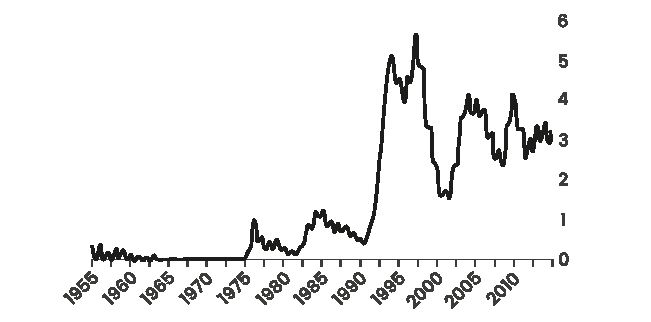
\includegraphics[width=\textwidth]{figures/fig7.pdf}
\caption[Werkloosheidspercentage in Zwitserland]{Werkloosheidspercentage in Zwitserland}
\label{fig7}
\end{figure}

In een vrije markt met gezond geld\index{gezond geld} neemt spaargeld gedurende de tijd in
marktwaarde toe, en hebben individuen de vrijheid om wel of niet te
werken. Ze kunnen elk gewenst loon vragen. Werkgevers hebben ook de
vrijheid om elk gewenst salaris te betalen. In zo'n
wereld waarin spaartegoeden\index{spaartegoeden} in waarde stijgen, is het volkomen rationeel
dat velen ervoor kiezen om geen werk te zoeken. Een werknemer die geen
werk kan vinden tegen een geldend loon, kan simpelweg niemand vinden die
de marginale opbrengst van zijn arbeid hoger waardeert dan de werknemer
zijn persoonlijke waardering van vrije tijd. Het moderne fenomeen van
massale, onvrijwillige werkloosheid is alleen mogelijk wanneer wetten,
regels of beperkingen bestaan die het illegaal en strafbaar maken om
arbeid te verrichten tegen specifieke loonniveaus.

In de context van vrije handel kan er onder mensen die bereid zijn om te
werken geen sprake zijn van werkloosheid, aangezien dat zou betekenen
dat ze recht hebben op een loon dat niemand bereid is hen te betalen. De
werknemer zou altijd werk kunnen vinden door zijn productiviteit te
verhogen of zijn gevraagde loon te verlagen. Gedwongen werkloosheid is
onmogelijk in een vrijemarkteconomie; het is de keuze van de werknemer
om een loon te vragen dat niemand bereid is te betalen, en daardoor is
het hun keuze om werkloos te blijven.

\section{Komt er ooit een einde aan werk?}

Arbeid is als productiemiddel uiterst waardevol, juist omdat het met
vrije tijd concurreert om het meest schaarse productiemiddel, de
menselijke tijd. Naarmate het inkomen en nut dat je door werk krijgt toeneemt, neemt de welvaart van werknemers toe. Dit stelt hen in staat
zich meer vrije tijd te veroorloven, maar het vergroot ook de
vermindering van het nut van hun arbeid en ontmoedigt hen om te werken.
Arbeid zou het enige economische goed of activiteit kunnen zijn waarvan
de geleverde hoeveelheid kan afnemen naarmate de prijs\index{prijs} stijgt. Dit komt
doordat een stijging van de arbeidsprijs leidt tot een toename van de
rijkdom van de werknemer, waardoor hij meer vrije tijd kan kopen en
minder arbeid hoeft te verkopen. De schaarste\index{schaarste} aan tijd betekent dat het
aanbieden van arbeid opportuniteitskosten met zich meebrengt die
toenemen naarmate een persoon meer verdient met werken. Deze dynamiek
heeft velen doen speculeren dat economische vooruitgang op een dag zou
kunnen betekenen dat mensen niet meer hoeven te werken.

Zullen we ooit een punt bereiken waarop we niet meer hoeven te werken?
Dit is een veel voorkomende fantasie onder politici en economen die niet
vertrouwd zijn met de economische manier van denken, zoals John Maynard
Keynes en zijn vele volgelingen. In de jaren `30 speculeerde Keynes dat
de productiviteit zo sterk zou blijven stijgen dat mensen tegen 2030
slechts 15 uur per week zouden moeten werken om te produceren wat ze
nodig hebben. Keynes fantaseerde dat technologische vooruitgang zou
leiden tot technologische werkloosheid, die hij definieerde als
`werkloosheid door onze ontdekking van middelen om sneller op het
gebruik van arbeid te besparen dan het tempo waarin we nieuwe
toepassingen voor arbeid kunnen vinden.'\autocite{43}

`Dit alles betekent op de lange termijn dat de mensheid haar economisch\index{economisch}
probleem oplost', concludeerde Keynes. Hij zag het economisch\index{economisch} vraagstuk
als een wiskundig probleem dat maar éénmaal opgelost hoeft te worden om
definitief opgelost te zijn. Hij ging ervan uit dat het vooral draaide
om het veiligstellen van een bepaalde verzameling goederen en diensten
die nodig zijn voor een gelukkig leven. Wanneer daar eenmaal voor was
gezorgd, zou het economisch\index{economisch} probleem voor eens en altijd zijn opgelost,
waardoor niemand ooit meer economisch\index{economisch} zou hoeven te handelen. In
werkelijkheid is het economisch\index{economisch} vraagstuk een permanent onderdeel van
het menselijk bestaan. We worden voortdurend geconfronteerd met keuzes
tussen schaarse dingen, omdat die schaarste\index{schaarste} voortkomt uit onze beperkte
en extreem kostbare tijd. Zolang mensen leven en moeten beslissen hoe ze
hun tijd willen besteden, zal het economische vraagstuk blijven bestaan
en zullen mensen het proberen op te lossen door te werken. Er kan geen
definitieve oplossing zijn voor het economisch\index{economisch} vraagstuk, alleen de
vervanging van slechte keuzes door betere keuzes.

`Ik concludeer dat, ervan uitgaande dat er geen belangrijke oorlogen en
geen belangrijke bevolkingsgroei zullen zijn, het economisch\index{economisch} probleem
binnen honderd jaar opgelost kan zijn, of op z'n minst
een oplossing in zicht is... Dus voor de eerste keer sinds zijn
schepping zal de mens worden geconfronteerd met zijn echte en permanente
probleem -- hoe hij zijn vrij zijn van dringende economische zorgen moet
gebruiken, hoe hij de vrije tijd, die wetenschap en samengestelde rente\index{rente}
hebben voortgebracht, moet besteden om wijs, aangenaam en goed te
leven.'\autocite{45}

Keynes lijkt zich niet bewust te zijn van het feit dat wat hij voorstelt
als een vervanging voor het economisch\index{economisch} probleem, gewoon het economisch\index{economisch}
probleem zelf is, maar dan toegepast op keuzes die iets anders zijn dan
die hij gewend was te zien in de zeer weinige economische boeken die hij
had gelezen. Het eeuwige en universele economische probleem van de mens
is hoe we onze tijd besteden, omdat tijd schaars is. De simplistische
opvatting van Keynes over de economie maakt het hem onmogelijk te
onderkennen dat het gebruik van tijd een economische keuze is.

Ongeacht hoeveel materiële dingen we hebben, we zullen altijd een keuze
moeten maken in de marge van directe en toekomstige voldoening. We
kunnen altijd huidige voldoening opgeven voor meer toekomstige
voldoening. Er zal nooit volledige voldoening zijn, omdat het menselijk
verstand altijd een betere mogelijkheid zal voorzien en ernaar zal
streven. Het zou voor iemand heel goedkoop zijn om vandaag te leven
volgens de levensstandaard van Keynes' tijd. Toch
kunnen zelfs de armste mensen vandaag de dag veel dingen gebruiken en
bezitten die Keynes nooit heeft kunnen bezitten. En ze blijven verlangen
naar een beter leven, net als de rijkste mensen. Zolang mensen
economisch\index{economisch} handelen, gebruiken ze hun verstand om nieuwe goederen,
diensten en objecten te produceren die anderen wensen.

Keynes baseert zijn fantasierijke visie van de toekomst op een volledig
ongegronde bewering dat er twee soorten behoeften zijn: absolute en
relatieve behoeften. Absolute behoeften, zo stelde Keynes, zijn
behoeften die we voelen `ongeacht de situatie van onze medemensen'.
Daarentegen worden relatieve behoeften alleen gevoeld `als hun
vervulling ons boven onze medemensen uit tilt, ons een gevoel van
superioriteit geeft'.\autocite{46} Keynes stelt dat de vraag naar het voldoen 
van het laatste wellicht onverzadigbaar zou kunnen zijn, maar dat aan de vraag 
naar de vervulling van de eerste klasse van behoeften volledig voldaan zou 
kunnen worden. Keynes dacht dat het economisch\index{economisch} probleem altijd het primaire en
dringendste probleem van het menselijk ras en het hele biologische rijk
is geweest. Het oplossen ervan zou een buitengewoon belangrijke
verandering in de aard van het menselijk leven betekenen. Hij begreep
echter niet dat het economisch\index{economisch} probleem altijd bestaat zolang menselijke
tijd schaars is en mensen keuzes moeten maken. Zelfs als mensen zich in
een denkbeeldige wereld bevonden waarin alles wat ze zich wensen
onmiddellijk wordt gerealiseerd, dan nog zou het economisch\index{economisch} probleem
niet zijn opgelost. De sterfelijkheid van de mensen dwingt hen nog
steeds om economisch\index{economisch} met hun schaarse tijd om te gaan. Het economisch\index{economisch}
probleem wordt elke seconde opgelost wanneer een mens nadenkt over zijn
tijd en een keuze maakt. Maar dan dient zich in de volgende seconde een
nieuw economisch\index{economisch} probleem aan dat dezelfde mens dwingt om opnieuw een
keuze te maken. De enige definitieve oplossing voor het economisch\index{economisch}
probleem is de dood, het moment waarop er geen verdere keuzes meer zijn
over de verdeling van de tijd.

Het is dus onzinnig om je zoals Keynes voor te stellen dat werk
ooit zou kunnen stoppen, of dat de behoefte aan werk ooit zou kunnen
verdwijnen, of dat overvloed een punt zou bereiken waarop arbeid niet
meer nodig is. We handelen voortdurend economisch\index{economisch} en we moeten altijd
keuzes maken tussen alternatieven. Naarmate onze levensstandaard
verbetert, verbeteren onze keuzes, maar het maken van keuzes moet
blijven bestaan, in ieder geval zolang mensen sterfelijk zijn.

\section{Is werk uitbuiting?}

Worden arbeiders uitgebuit door het kapitalisme\index{kapitalisme}? Er zijn miljoenen
pagina's geschreven over het onderwerp van uitbuiting
van arbeiders, voornamelijk gebaseerd op het onsamenhangende gewauwel
van Karl Marx. Marx was een semi-geletterde Duitse zwerver die nooit een
baan had die hem kon onderhouden. Marx leefde van de steun van rijke weldoeners 
terwijl hij orakelde over het herontwerpen van de wereld tot een dystopie, 
geleid door mensen die niet in staat zijn zichzelf te onderhouden door hun eigen arbeid.

Marxistische economische analyse is gebaseerd op de arbeidswaardeleer,
besproken in Hoofdstuk 2. Aangezien alle economische goederen arbeid
vereisen om ze te veranderen in bruikbare economische goederen,
concludeert de marxist ten onrechte dat arbeid economische goederen
waarde geeft en dat de hoeveelheid arbeid die voor de productie\index{productie} van een
goed gebruikt wordt, de waarde ervan bepaalt. Dit betekent dat de waarde
van goederen is gebaseerd op de hoeveelheid arbeid die nodig is voor hun
productie\index{productie}. Door de ongegronde aanname te gebruiken dat economische
waarde puur wordt toegekend aan objecten op basis van de hoeveelheid
arbeid die in hen wordt gestopt, schakelt de marxist automatisch de
waarde van de bijdrage van de kapitalist uit. De arbeiders moeten komen
opdagen en werken, terwijl de kapitalisten, zoals de socialisten
beweren, niets doen. Volgens dit standpunt exploiteert de kapitalist de
arbeider, omdat de arbeider niet de volledige winst ontvangt van het
productieproces\index{productieproces}.

De bewering dat werknemers geen keuze hebben dan voor kapitalisten te werken, is duidelijk incorrect. Werknemers maken immers vrijwillig de keuze om voor deze zogenaamde uitbuiters te werken, een feit dat marxisten vaak negeren. Zolang kapitalisten geen geweld of dreiging met geweld gebruiken om werknemers te dwingen voor hen te werken, is de keuze van werknemers om werk te aanvaarden een indicatie dat zij het zien als de beste manier om hun tijd te besteden. Hoewel buitenstaanders of economen deze situatie misschien betreurenswaardig vinden, kunnen zij kapitalisten niet verwijten dat zij werknemers de beste beschikbare optie bieden in ruil\index{ruil} voor hun tijd. Het is opmerkelijk dat marxisten die kritiek hebben op deze verhoudingen niet in staat zijn om werknemers betere arbeidsmogelijkheden te bieden dan de zogenaamde kapitalistische `uitbuiters'.

Het zien van arbeid als een vorm van uitbuiting toont een diep gebrek aan begrip over de essentie en de waarde van kapitaal\index{kapitaal} voor economische productie\index{productie}. Kapitalisten kiezen ervoor hun consumptie\index{consumptie} uit te stellen om werknemers van kapitaal\index{kapitaal} te voorzien, wat de productiviteit van de werknemers verhoogt. Ze staan voortdurend voor de keuze om consumptie\index{consumptie} uit te stellen ten behoeve van het verschaffen van kapitaal\index{kapitaal} aan werknemers. Immers, kapitalisten hebben de mogelijkheid hun kapitaalgoederen\index{kapitaalgoederen} op ieder moment te liquideren en de opbrengsten te besteden aan consumptie\index{consumptie}. Door de keuze te maken consumptie\index{consumptie} uit te stellen en kapitaal\index{kapitaal} ter beschikking te stellen, maakt de kapitalist het mogelijk voor een werknemer om een hogere productiviteit te bereiken. Dit hogere niveau van productiviteit zorgt ervoor dat de werknemer tevreden is, ook al ontvangt hij slechts een deel van de opbrengst. Het alternatief voor deze zogenaamde kapitalistische uitbuiting is niet dat de werknemer alle inkomsten uit de verkoop van de geproduceerde goederen krijgt; het alternatief zou zijn dat de opbrengsten aanzienlijk lager zijn zonder de inbreng van kapitaal\index{kapitaal}. Een marxist zou kunnen beweren dat een taxichauffeur uitgebuit wordt door de eigenaar van de auto die hij bestuurt, maar dit perspectief miskent wat er zou gebeuren als de chauffeur geen vergoeding zou betalen voor het gebruik van de auto. Zonder een rendement op zijn investering te ontvangen, zou de kapitalist de auto liever als een consumptiegoed\index{consumptiegoed} inzetten of verkopen om de opbrengst te consumeren. Zonder toegang tot de auto zou de chauffeur genoodzaakt zijn mensen op zijn rug te vervoeren, een uiterst inefficiënte en fysiek belastende manier van werken. Het is pas door de zogenaamde 'uitbuiting' door een kapitalist, die hem van kapitaal\index{kapitaal} (de auto) voorziet, dat de arbeid van een chauffeur productief en veilig genoeg wordt om hem een fatsoenlijk leven te bieden.

Het productieproces\index{productieproces} vraagt niet alleen om de tijd van de werknemer, maar ook om de bijdrage van kapitaal\index{kapitaal} door de kapitalist. Dit kapitaal\index{kapitaal} kan alleen verkregen worden door arbeid die al eerder is verricht en kan alleen behouden blijven door consumptie\index{consumptie} gedurende het gehele productieproces\index{productieproces} continu uit te stellen. Zonder compensatie voor de kapitalist voor haar keuze om bevrediging uit te stellen en te investeren, zou er geen kapitaal\index{kapitaal} beschikbaar zijn, wat de productiviteit van de werknemer aanzienlijk zou verminderen. De kapitalist exploiteert de werknemer niet door een deel van zijn productie\index{productie} op te eisen; in plaats daarvan betaalt de werknemer vrijwillig een deel van zijn productie\index{productie} aan de kapitalist, als ruil\index{ruil} voor een veel hoger niveau van productiviteit.

De relatie tussen arbeider en kapitalist is een kenmerk van menselijke
relaties dat in alle menselijke culturen heeft bestaan. Het weerspiegelt
een natuurlijke ruil\index{ruil} tussen een individu dat de capaciteit heeft
om te werken, maar niet de middelen heeft om het noodzakelijke kapitaal\index{kapitaal}
veilig te stellen, en een ander individu dat meer kapitaal\index{kapitaal} heeft dan ze
kan of wil benutten. Het voortbestaan van deze relatie is wat mensen
aanzet tot het vergaren van kapitaal\index{kapitaal}. Het pathologiseren en bestraffen
ervan heeft echter geleid tot een rampzalige economische vernietiging in
samenlevingen.

\chapter{Eigendom}

\begin{blockquotebox}
    Alleen omdat er schaarste\index{schaarste} bestaat, is er een probleem bij het formuleren van morele wetten; want zodra goederen in overvloed (\enquote{vrije} goederen) aanwezig zijn, doet het conflict over het gebruik ervan zich niet voor en is coördinatie overbodig. Hieruit volgt dat een juist begrepen ethiek geformuleerd moet worden als een eigendomstheorie, dat wil zeggen, een theorie over het toekennen van exclusieve controlerechten over schaarse middelen. Dit is de enige manier om anders onvermijdelijke en onoplosbare conflicten te voorkomen.\footnotemark
    \par\raggedleft--- Hans-Hermann Hoppe\index{Hans-Hermann Hoppe}
\end{blockquotebox}
\footautocite{47}


\section{Schaarste en eigendom}

\lettrine{H}oofdstuk 3 behandelde het proces van economisch\index{economisch} handelen als gevolg van de schaarste\index{schaarste} van menselijke tijd. Hoofdstuk 4 onderzocht hoe mensen hun tijd economiseren door een keuze te maken tussen vrije tijd en arbeid, en legde de basisprincipes uit van het productieproces\index{productieproces}. Hoofdstuk 5 onderzoekt het proces van economisch\index{economisch} handelen met goederen en de economische reden voor het ontstaan van eigendom. Na uitleg over de economische betekenis van eigendom, behandelt dit hoofdstuk verschillende soorten eigendom, de toepassing van eigendom op zelfbeschikking en hoe eigendom als instituut helpt in de eeuwige zoektocht om de waarde en hoeveelheid menselijke tijd te vergroten.

Zoals besproken in het eerste hoofdstuk van dit boek, is schaarste\index{schaarste} het startpunt van economie en de oorsprong van al het economisch\index{economisch} handelen. Het is het verschil tussen de gewenste en beschikbare hoeveelheid van een goed dat mensen dwingt om zorgvuldig met dat goed om te gaan, het in optimale conditie te houden om zijn functies te kunnen vervullen, en het te beschermen tegen het feit dat anderen het voor zichzelf kunnen nemen. Schaarste is wat ons dwingt om objecten te waarderen en door ze te waarderen ontwikkelen we er in de loop van de tijd controle over. Schaarste is dan ook de oorsprong van eigendom. Zoals Menger uitlegt:

\begin{blockquotebox}
    Eigendom is net zoals de menselijke economie geen toevallige uitvinding. Het is eerder de enige praktisch mogelijke oplossing voor het probleem dat door de aard der dingen aan ons wordt opgelegd door het verschil tussen de behoeften aan, en de beschikbare hoeveelheden van alle economische goederen.\footnotemark
\end{blockquotebox}
\footautocite{48}


Een goed in eigendom hebben betekent de volledige controle uitoefenen over de diensten die daaruit kunnen voortvloeien. Menger definieert eigendom als \enquote{de totale som van goederen waarover een economisch\index{economisch} handelend individu volledige beschikkingsmacht heeft voor de voldoening van zijn behoeften.}\autocite{49} De wetsgeleerde A. N. Yiannopolous schrijft:

\begin{blockquotebox}
    Eigendom kan worden gedefinieerd als een exclusief recht om de controle uit te oefenen over een economisch\index{economisch} goed...; het is de naam van een concept dat verwijst naar de rechten en verplichtingen, privileges en beperkingen die de relatie van de mens met waardevolle dingen bepalen. Mensen verlangen overal en altijd naar het bezit van dingen die noodzakelijk zijn voor overleving of waardevol zijn volgens culturele normen en die, als gevolg van de vraag naar die zaken, schaars worden. Wetten, die worden afgedwongen door een georganiseerde samenleving, regelen de competitie om deze gewenste dingen en garanderen het genot ervan. Wat gegarandeerd van iemand is, is eigendom. [Eigendomsrechten] verlenen een direct en onmiddellijk gezag over een ding.\footnotemark
    \par\raggedleft--- Hans-Hermann Hoppe\index{Hans-Hermann Hoppe}
\end{blockquotebox}
\footautocite{50}

Eigendom is iets anders dan rijkdom, wat Menger definieert als \enquote{de volledige som van economische goederen die ter beschikking staan van een economisch\index{economisch} handelend individu.} \autocite{51} Iemands eigendom bevat ook alle niet-economische goederen, maar rijkdom verwijst alleen naar economische goederen.

De economische reden voor het hebben van eigendom is duidelijk en eenvoudig. Als het gebruik van een economisch\index{economisch} goed het niet verbruikt en het niet onbruikbaar maakt, kan het opnieuw worden gebruikt voor hetzelfde doel. De gebruiker zou het dan ook vanzelfsprekend het in eigendom willen houden tot hij of zij het weer nodig heeft. Een jager die een speer maakt om een konijn te doden, zal instinctief begrijpen dat de speer opnieuw kan worden gebruikt om een ander konijn te jagen en zal ervoor kiezen de speer in zijn bezit te houden. Heel weinig dieren hebben het instinct om objecten in bezit te nemen en misschien nemen niet-menselijke soorten alleen maar eigendom van hun woonplaatsen, nesten of holen. Door het superieure intellect van de mens kunnen wij op een veel meer verfijnde en complexe manier een bezitsdrang ontwikkelen en blijven dingen voor jaren, decennia en zelfs eeuwen het eigendom van meerdere generaties van dezelfde familie.

Door waardevolle objecten in eigendom te nemen, kunnen mensen de kosten en tijd die nodig zijn om toekomstige taken uit te voeren, verminderen. De eigenaar van duurzame goederen kan haar doel bereiken met minder inspanning en kosten dan iemand die niet hetzelfde eigendom heeft. Het investeren van arbeid in het bouwen van een degelijk huis voor de langere termijn is een effectievere manier om onderdak te regelen dan elke dag een nieuwe provisorische oplossing te zoeken. Het temmen en houden van dieren kan een betrouwbaardere manier zijn om voedsel te verkrijgen, dan elke dag te moeten jagen. Het cultiveren van je eigen bomen en gewassen kan betrouwbaarder en productiever zijn dan het elke dag zoeken naar planten. Dit zijn allemaal methoden waarmee mensen economiseren om hun overlevingskansen te verbeteren en de waarde van hun tijd te verhogen, met andere woorden, de hoeveelheid en de waarde van de tijd die ze op aarde hebben te vergroten.

We kunnen eigendom ook zien als een manier om de tijd die aan arbeid wordt besteed om te zetten in toekomstig nut. Door zijn arbeid te gebruiken om een duurzaam goed te produceren, ziet de mens af van directe voldoening, om zo een goed te maken dat continu nut levert over een toekomstige periode. De meest basale behoeften van de mens kunnen effectiever worden vervuld door te investeren in duurzaam eigendom. Het besteden van arbeid aan het bewerken van een stuk grond geeft een reden om op dat stuk grond te blijven en er blijvend van te profiteren. Het bezit van land maakt een langetermijninvestering en de verhoging van het nut mogelijk, meer dan wanneer het zonder eigenaar bleef, omdat het gebrek aan eigendom investeringen ontmoedigt.

Het belang van eigendom binnen de sociale context is dat het conflicten over schaarse middelen voorkomt. Zoals Stephan Kinsella het verwoordt:

\begin{blockquotebox}
    Er is altijd de mogelijkheid van conflict over betwistbare (schaarse) middelen. Dit zit in de aard van schaarse of concurrerende middelen. Door aan elk goed een eigenaar toe te wijzen, stelt het juridische systeem van eigendomsrechten objectieve, publiekelijk zichtbare of waarneembare grenzen vast waar niet-eigenaars zich aan kunnen houden.\footnotemark
\end{blockquotebox}
\footautocite{52}


\section{Soorten eigendom}

Fysieke goederen kunnen worden geclassificeerd in vier types: bederfelijke goederen, duurzame goederen, kapitaalgoederen\index{kapitaalgoederen} en monetaire goederen. Consumptiegoederen zijn de uiteindelijke doelen van het economisch\index{economisch} handelen, ofwel de goederen die mensen aanschaffen voor eigen gebruik. Duurzame consumptiegoederen\index{consumptiegoed} onderscheiden zich van bederfelijke consumptiegoederen\index{consumptiegoed} doordat ze lange perioden in bezit worden gehouden, omdat hun consumptie\index{consumptie} over een langere duur kan worden uitgespreid. Voorbeelden van duurzame consumptiegoederen\index{consumptiegoed} zijn huizen, auto's, televisies, of wasmachines. Kapitaalgoederen zijn goederen die worden aangekocht vanwege hun vermogen om consumptiegoederen\index{consumptiegoed} te produceren. Monetaire goederen zijn goederen die niet worden bewaard om te consumeren of om consumptiegoederen\index{consumptiegoed} mee te produceren, maar om later te worden ingewisseld voor andere goederen.

In een sociaal systeem dat bevorderlijk is voor individuen die economiseren en zo veel mogelijk conflicten proberen te vermijden, kunnen eigendomsclaims worden vastgesteld op basis van \enquote{het bestaan van een objectieve en intersubjectief verifieerbare link tussen de eigenaar en het geclaimde hulpmiddel}, zoals Hoppe het zegt.\autocite{53} In een vrije markt, of in een sociale orde zonder dwang, zijn er drie manieren voor individuen om legitiem eigendom te verwerven, zoals Rothbard uitlegt:

\begin{enumerate}
\def\labelenumi{\arabic{enumi}.}
\item Het claimen van objecten die nog geen eigenaar hebben
\item Producten die afgeleid zijn van deze objecten
\item Objecten op vrijwillige basis verkregen van rechtmatige eigenaren, \\hetzij door (ruil\index{ruil})handel, hetzij als een geschenk.
\end{enumerate}

\section{Zelfbeschikking}

Omdat mensen schaars zijn, en hun tijd ook, is het alleen maar vanzelfsprekend dat dezelfde implicaties van schaarste\index{schaarste} voor economische goederen ook op mensen van toepassing zijn. Eigendom is volgens Menger de \enquote{enige praktische oplossing}. Hoewel het idee van eigendom van mensen schokkend en moreel verkeerd klinkt, is het in economische termen onvermijdelijk. Aangezien mensen en hun tijd schaars zijn, moeten de beslissingen over hoe een mens zich gedraagt en wat hij met zijn tijd doet door iemand worden genomen. Dat is de essentie van eigendom. De persoon die beslist wat er met het lichaam en de tijd van een persoon moet gebeuren, bezit \emph{de facto} deze economisch\index{economisch} gezien. De kwalificatie \enquote{afschuwelijk} is alleen van toepassing en gepast wanneer de vraag naar eigendom in het voordeel van iemand anders dan de persoon zelf wordt beantwoord.

Er zijn slechts drie mogelijke manieren om het eigendom van mensen te regelen:

\begin{enumerate}
\def\labelenumi{\arabic{enumi}.}
\item Via zelfbeschikking, waarbij een persoon zichzelf volledig bezit en anderen geen eigendomsrechten kunnen claimen over zijn lichaam en tijd.
\item Gemeenschappelijk eigendom, waarbij alle leden van de samenleving gezamenlijk al hun lichamen bezitten en gezamenlijk beslissen wat elk lichaam doet.
\item Slavernij, waarin een persoon het eigendom is van iemand anders en zijn eigenaren bepalen wat ze kunnen doen met het lichaam en de tijd van de slaaf. Dit varieert van het toewijzen van zijn tijd aan taken tot het toebrengen van lichamelijke schade. De rechten van slaveneigenaren gaan zelfs zo ver dat ze de slaaf mogen vermoorden. In een sociale orde met slavernij hebben sommige mensen eigendomsrecht over zowel zichzelf als anderen, terwijl anderen geen recht van eigendom hebben over zichzelf of anderen.
\end{enumerate}


De tweede optie is praktisch niet werkbaar buiten de omvang van een handjevol mensen die elkaar goed kennen, en zelfs dan zou het niet gemakkelijk zijn. Mensen zouden het erg moeilijk vinden om alle kennis te vergaren om te beslissen wat anderen met hun leven en tijd zouden moeten doen. De problemen om een mechanisme te bedenken voor informatieoverdracht, besluitvorming en uitvoering in een grootschalig sociaal systeem zijn praktisch onoverkomelijk.

De derde optie faalt op het gebied van consistentie, ethiek en al de gevolgen. Wat voor ethische basis kan er zijn om te rechtvaardigen waarom sommige mensen van zichzelf zijn, terwijl anderen in eigendom zijn van anderen? Er kan geen logisch en ethisch samenhangende manier zijn om dit drastisch verschil in toewijzing van eigendomsrechten te rechtvaardigen. Verder is dit verschil waarschijnlijk een recept voor conflicten. Het individu dat geen zelfeigendomsrechten heeft, zal proberen deze te verkrijgen en kan zich gerechtvaardigd voelen in het gebruik van geweld tegen degenen die hem bezitten. Overal waar slavernij als systeem heeft bestaan, heeft het geleid tot conflict.

Persoonlijke zelfbeschikking is de enige logische en ethisch consistente oplossing voor het probleem van menselijk eigendom, en het is de enige die waarschijnlijk zal leiden tot vreedzame samenwerking in plaats van gewelddadig conflict. Zelfbeschikking betekent dat een individu volledige aanspraak heeft op zijn eigen lichaam en tijd. Wanneer we het principe van zelfbeschikking accepteren, ontstaat er een coherent kader voor het begrijpen van rechten, rechtvaardigheid en non-agressie. Dit principe strekt zich uit tot wat een mens kan produceren als gevolg van deze keuzes, ofwel eigendom. Je kunt agressie zien als het gebruik of de dreiging van geweld om het lichaam of de tijd van een ander persoon te beheersen, en elke fysieke agressie tegen een individu zou een schending zijn van zijn recht op zelfbeschikking.

Als we eigendomsrechten begrijpen als de enige werkende oplossing voor economische schaarste\index{schaarste} en als we vrede en beschaving\index{beschaving} waarderen, is het moeilijk om tegen zelfbeschikking en het systeem van eigendomsrechten te argumenteren. Elk dergelijk argument kan gezien worden als doorzichtig egoïstische hypocrisie. In plaats van een intelligent argument dat voortkomt uit het menselijk verstand, is dit argument niets meer dan een oproep om terug te keren naar de zeden van dieren die volledig door hun instincten worden beheerst, en niet in staat zijn om hun verstand te gebruiken. Argumenteren tegen zelfbeschikking is feitelijk argumenteren tegen je eigen persoonlijke identiteit, omdat het duidelijk maakt dat je geen respect hebt voor eigendomsrechten en geen deel kunt zijn van een beschaafde sociale orde. Het is een pleidooi om als een dier beschouwd te worden. Hoewel economische theorie geen politieke ideologie voorschrijft, zal begrip van economische schaarste\index{schaarste} en een waardering van vrede en beschaving\index{beschaving} een persoon ertoe aanzetten een libertarische kijk aan te nemen. Voor zelfbeschikking bestaan geen alternatieven die niet tot conflict leiden en geen vijandigheid en wrok tussen individuen en groepen creëren.

Hoewel de meeste ideologieën niet expliciet voor slavernij zullen pleiten, volgen alleen libertariërs deze norm strikt tot in al zijn logische consequenties. Alle andere ideologieën geloven in minimaal een bepaalde vorm van slavernij, in de vorm van een legitieme aanspraak van anderen op iemands lichaam of tijd. Voorstanders van belasting, dienstplicht, drugsverboden of medische mandaten vinden het misschien niet leuk om zichzelf te zien als voorstanders van slavernij, maar ze geven een gedeeltelijk eigendomsrecht over iemands lichaam in handen van de staat. Ze doen dit omdat ze de staat steunen als ze haar burgers als eigendom behandelt. Dit gebeurt wanneer de staat hun inkomen met geweld afneemt, ze in de gevangenis opsluit voor het consumeren van drugs, of hen uitsluit van werk voor het niet gebruiken van door de staat verplichte farmaceutische producten.\autocite{54}

\section{Belang van eigendomsrechten}

Door het concept eigendom te begrijpen, kan een individu beter en effectiever economiseren, en de productiviteit en waarde van zijn tijd verhogen. Door zijn arbeid te investeren in de productie\index{productie} van duurzame goederen, kan een mens langer van hun diensten profiteren. Dit verlaagt zijn tijdsvoorkeur\index{tijdsvoorkeur} en hij leert meer prioriteit te geven aan de toekomst.

Wanneer het accepteren van eigendomsrechten de geldende norm wordt in een samenleving, zijn individuen in staat om in kapitaalgoederen\index{kapitaalgoederen} te investeren om met anderen te handelen. Hun productiviteit neemt verder toe en de economische marktorde ontwikkelt zich. Dit wordt besproken in de volgende hoofdstukken. Eigendomsrechten kunnen worden begrepen als het sociale mechanisme dat mensen in staat stelt om hun eigendom te behouden in de nabijheid van anderen die het misschien ook willen bezitten. Zoals Mises het verwoordde, \enquote{privaat eigendom van de productiemiddelen is het fundamentele instituut van de markteconomie. Het is de instelling wiens aanwezigheid de markteconomie kenmerkt. Waar het afwezig is, is er geen sprake van een markteconomie.}\autocite{55}

De markteconomie en de beschaving\index{beschaving} zelf zijn gebaseerd op het respect voor eigendomsrechten. Het is alleen bij veilige eigendomsrechten dat mensen een hoeveelheid kapitaal\index{kapitaal} kunnen vergaren die significant groter is dan wat ze bij zich kunnen dragen voor hun eerste levensbehoeften. Een samenleving waarin eigendomsrechten niet worden gerespecteerd is er een waarin veel conflicten zijn. In zo'n maatschappij kunnen individuen zich niet veroorloven om hun kostbare arbeid in de toekomst te investeren, omdat al het eigendom dat deze waarde kan opslaan, riskant is om te bezitten. Een beschaafde samenleving is alleen mogelijk wanneer het recht op eigendom van jezelf en objecten in brede kring wordt gerespecteerd. Mensen kunnen dan verwachten hun eigendom zeker te stellen voor de toekomst.

In de context van een markteconomie legt Mises op prachtige wijze uit hoe het instituut van privaat eigendom zorgt voor een verantwoord beheer van middelen:

\begin{blockquotebox}
    De betekenis van privaat eigendom in de marktsamenleving is radicaal anders dan onder een systeem van autarkie van elk huishouden. In een situatie waarin elk huishouden economisch\index{economisch} zelfvoorzienend is, dienen de productiemiddelen van het private eigendom uitsluitend de eigenaar. Alleen dit huishouden plukt de vruchten van het gebruik. In de marktsamenleving kunnen de eigenaren van kapitaal\index{kapitaal} en land alleen genieten van hun eigendom door het te gebruiken om aan de behoeften van anderen te voldoen. Ze moeten in dienst zijn van de consumenten om enig voordeel te hebben van wat van hen is. Het feit dat ze productiemiddelen bezitten, dwingt hen zich te onderwerpen aan de wensen van het publiek. Eigendom is alleen een voordeel voor degenen die weten hoe ze het op de best mogelijke manier kunnen gebruiken ten behoeve van de consumenten. Het is een sociale functie.\footnotemark
\end{blockquotebox}
\footautocite{56}

De afwezigheid van privaat eigendomsrecht leidt tot conflicten tussen mensen, evenals tot de teloorgang van economische goederen en natuurlijke hulpmiddelen. Wanneer economische goederen geen duidelijke eigendomsrechten hebben, zullen de individuen die ze op enig moment gebruiken en beheren, dit doen zonder de verwachting ze in de toekomst te kunnen gebruiken. Dit leidt ertoe dat ze de toekomstige staat van deze middelen niet als prioriteit zien. Deze sterke onderwaardering van de toekomst is een kenmerkend aspect van het gebruik van goederen zonder een duidelijke eigenaar. Privaat eigendom motiveert eigenaars om zich te bekommeren om de staat van hun eigendom over de lange termijn.


Zoals Mises uitlegt:

\begin{blockquotebox}
    Als land in niemands bezit is, terwijl het formeel wettelijk als publiek eigendom kan worden beschouwd, wordt het gebruikt zonder enige aandacht voor de resulterende nadelen. Personen die in staat zijn om de opbrengsten voor zichzelf toe te eigenen -- het hout en wild uit de bossen, vis uit wateren en minerale afzettingen uit de bodem -- maken zich niet druk over de effecten van hun exploitatiemethoden op langere termijn. Erosie van de bodem, uitputting van eindige bronnen en andere schadelijke effecten op het toekomstig gebruik worden door hen gezien als externe kosten die geen deel uitmaken van hun berekening van input en output. Ze kappen bomen zonder nieuwe scheuten of herbebossing te overwegen. Bij jagen en vissen schrikken ze niet terug voor methoden die herbevolking van de jacht- en visgronden onmogelijk maken. In de vroege dagen van de menselijke beschaving\index{beschaving}, toen er nog volop grond van goede kwaliteit beschikbaar was, zagen mensen dergelijke roofzuchtige methoden niet als een probleem. Toen de effecten merkbaar werden in een afname van de netto-opbrengsten, verliet de boer zijn boerderij en verhuisde hij naar een andere plek. Pas als een land dichter bevolkt raakte en er geen ongebruikt land van topkwaliteit meer beschikbaar was, begonnen mensen dergelijke roofzuchtige methoden als verspilling te beschouwen. Op dat moment consolideerden ze het instituut van privaat eigendom van land. Ze begonnen met landbouwgrond en stapten vervolgens over op weiden, bossen en visgebieden.\footnotemark
\end{blockquotebox}
\footautocite{57}


\part{The Market Order}
\part{Monetary Economics}
\part{Civilization}

\backmatter

% Graphics
% \chapter*{Overzicht van figuren}
% \addcontentsline{toc}{chapter}{Overzicht van figuren}
% \listoffigures

% tables
% \chapter*{Overzicht van tabellen}
% \addcontentsline{toc}{chapter}{Overzicht van tabellen}
% {\listoftables\newpage
% %remove empty page between list of tables and index
% \let\newpage\relax

 % bibliography
\nocite{*} % This will display all entries in the .bib file regardless of whether they're cited in the text
\printbibliography

% index
\makeoddhead{mystyle}{}{{\small{Index}}}{}
\printindex
\addcontentsline{toc}{chapter}{Index}

\end{document}
% END THE DOCUMENT